%%%%%%%%%%%%%%%%%%%%%%%%%%%%%%%%%%%%%%%%%%%%%%%%%%%%%%%%%%%%%%%%%%%%%%%%%%%%%%%%
%%
%%   BornAgain User Manual
%%
%%   homepage:   http://www.bornagainproject.org
%%
%%   copyright:  Forschungszentrum Jülich GmbH 2015
%%
%%   license:    Creative Commons CC-BY-SA
%%   
%%   authors:    Scientific Computing Group at MLZ Garching
%%               C. Durniak, M. Ganeva, G. Pospelov, W. Van Herck, J. Wuttke
%%
%%%%%%%%%%%%%%%%%%%%%%%%%%%%%%%%%%%%%%%%%%%%%%%%%%%%%%%%%%%%%%%%%%%%%%%%%%%%%%%%


\chapter{Particle form factors}  \label{SFF}

\makeatletter
\renewcommand{\@thesubfigure}{\relax}
\makeatother

\index{Form factor|(}

%%%%%%%%%%%%%%%%%%%%%%%%%%%%%%%%%%%%%%%%%%%%%%%%%%%%%%%%%%%%%%%%%%%%%%%%%%%%%%%%
\section{Shape transforms}
%%%%%%%%%%%%%%%%%%%%%%%%%%%%%%%%%%%%%%%%%%%%%%%%%%%%%%%%%%%%%%%%%%%%%%%%%%%%%%%%

\index{Shape transform|(}
The form factor of a particle is the Fourier transform
of its shape function,
\begin{equation}
  F(\q)=\int {\rm d}^3r\, {\rm e}^{i\q\r} S(\r).
\end{equation}
For hard-shell particles the shape function $S(\r)$
only takes the values 0 and~1
so that the form factor becomes
the \textit{shape transform}
\begin{equation}\label{eq:FFHard}
  F(\q)=\int_V {\rm d}^3r\, {\rm e}^{i\q\r},
\end{equation}
where $V$ is the volume of the particle.
\nomenclature[2v130 0]{$V$}{Volume of embedded particle}%

\BornAgain\ comes with a collection of hard-coded 
shape transform for standard particle geometries like
spheres, cylinders, prisms, pyramids or ripples.
This collection is documented in the following.
For each shape,
the real-space geometry is shown in orthogonal projections,
the parameters of the \BornAgain\ method are defined,
an analytical expression for the form factor is given,
and exemplary results for $\left|F(\q)\right|^2$ versus
$\alpha_\tf,\phi_\tf$ are shown for small-angle scattering conditions
($\alpha_\ti=\phi_\ti=0$).

The computation of $F(\q)$ is based on
shapes $S(\r)$ given in Cartesian coordinates,
as defined in the orthogonal projections.
Typically, the vertical ($z$) direction is chosen
along a symmetry axis of the particle.
The origin is always at the center of the bottom side of the particle.
Different parametrization or a different choice of the origin
cause our analytic form factors to trivially deviate
from expressions given in the \IsGISAXS\ manual \cite[Sect.~2.3]{Laz08}
or in the literature \cite[Appendix]{ReLL09}.

We recomputed all expressions to make sure
that they also hold for complex scattering vectors,
used to describe in order to take any material absorption into account.
The implementation in \BornAgain\ allows all three components
of~$\q$ to be complex.
According to Sect.~\ref{Smulayabs},
only the vertical components of $\k_\ti$ and $\k_\tf$ can have imaginary parts.
However,
to account for a tilt of the particle,
it may be necessary to evaluate $F(\v{\tilde q})$ with
a rotated scattering vector~$\v{\tilde q}$
that has complex $\tilde q_x$ or~$\tilde q_y$.

\E{Ripples}
\index{Ripple (form factor)}%
 are particles with infinite extension in one dimension
(by convention in $x$ direction).
They have the shape transform 
\begin{equation}\label{eq:FFHard}
  F(\q)=\delta(q_x)\int_A {\rm d}^2r\, {\rm e}^{i(q_x x+q_y y)},
\end{equation}
where $A$ is the cross section.
To avoid an extra distinction of cases,
\BornAgain\ requests that ripples have a \E{finite} length~$L$,
which users may keep fixed at a very large value.

The following tables summarize the implemented particle geometries,
 ordered by ascending number of parameters.
Afterwards, the detailed documentation is in alphabetical order.

\def\entry#1#2#3#4{%
\raisebox{-3.8ex}{\includegraphics[width=5em]{fig/blue/#2.png}} &
\texttt{#1} &
#4 &
Page~\pageref{sec:#3}, Sect.~\ref{sec:#3}\\}
\begin{center}
\small
\begin{longtable}
  {@{}p{.15\textwidth}
   @{}p{.35\textwidth}
   @{}p{.2\textwidth}
   @{}p{.25\textwidth}@{}}
Shape&Name&Parameters&Reference\\\hline
\entry{FullSphere}{FullSphere3d}{FullSphere}{$R$}
\hline
\entry{FullSpheroid}{FullSpheroid3d}{FullSpheroid}{$R$, $H$}
\entry{TruncatedSphere}{Sphere3d}{TruncatedSphere}{$R$, $H$}
\entry{Cylinder}{Cylinder3d}{Cylinder}{$R$, $H$}
\entry{Prism3}{Prism33d}{Prism3}{$L$, $H$}
\entry{Prism6}{Prism63d}{Prism6}{$R$, $H$}
\entry{TruncatedCube}{TruncatedCube3d}{TruncatedCube}{$L$, $t$}
\hline
\entry{EllipsoidalCylinder}{EllipsoidalCylinder3d}{EllipsoidalCylinder}{$R_a$, $R_b$, $H$}
\entry{HemiEllipsoid}{HemiEllipsoid3d}{HemiEllipsoid}{$R_a$, $R_b$, $H$}
\entry{TruncatedSpheroid}{Spheroid3d}{TruncatedSpheroid}{$R$, $H$, $f_p$}
\entry{Cone}{Cone3d}{Cone}{$R$, $H$, $\alpha$}
\entry{Box}{Box3d}{Box}{$L$, $W$, $H$}
\entry{Pyramid}{Pyramid3d}{Pyramid}{$L$, $H$, $\alpha$}
\entry{Tetrahedron}{Tetrahedron3d}{Tetrahedron}{$L$, $H$, $\alpha$}
\entry{Cone6}{Cone63d}{Cone6}{$R$, $H$, $\alpha$}
\entry{Ripple1}{Ripple13d}{Ripple1}{$L$, $W$, $H$}
\hline
\entry{AnisoPyramid}{AnistropicPyramid3d}{AnisoPyramid}{$L$, $W$, $H$, $\alpha$}
\entry{Cuboctahedron}{Cuboctahedron3d}{Cuboctahedron}{$L$, $H$, $r_H$, $\alpha$}
\entry{Ripple2}{Ripple23d}{Ripple2}{$L$, $W$, $H$, $d$}
\hline
\end{longtable}
\end{center}

In the following subsections,
information about the implemented geometries is given in standardized form.
Analytical expressions are given for the form factor $F(\q)$,
for the volume $V=F(0)$,
and for the maximum horizontal section $S$
(the area of the particle as seen from above).
\nomenclature[2s130 0]{$S$}{Maximum horizontal section of embedded particle}%
Mathematical notation in the form factor expressions includes
the cardinal sine functions $\sinc(z)\coloneqq\sin(z)/z$
and the Bessel function of first kind and first order $J_1(z)$
\cite[Ch.~9]{AbSt64}.
\nomenclature[2j132 01]{$J_1$}{Bessel function of first kind and first order}%
If results contain an integral,
then no analytical form was found,
and the integral is evaluated by numeric quadrature.
\index{Quadrature}%
The analytical expressions for $F(\q)$ contain singularities for
certain values of $\q$.
All these singularities are removable.
Our implementation comprises appropriate case distinctions.

Geometrical objects can be parametrized in different ways.
Concerns about user experience and about code readability
sometimes lead to different choices.
For the \BornAgain\ user interfaces (GUI and API)
we have chosen the most standard parameters,
as used in elementary geometry, like length, height, radius,
even if this is at variance from the \IsGISAXS\ precedent.
Where our parametrization made analytic expressions too tedious,
we use alternate internal parameters to alleviate the formul\ae.

Examplary form factors are numerically computed in Born approximation.
The particles are assigned a refractive index of $n=10^{-5}$.
The incident wavelength is 1~\AA.
The incident beam is always in the $xz$ plane, hence $\phi_\ti=0$.
Unless otherwise said, the incident glancing angle is $\alpha_\ti=1^\circ$.


%-------------------------------------------------------------------------------
% Start the series of standardized double pages.
\ifodd\value{page}\else\FloatBarrier\newpage\textit{Page intentionally left blank}\fi
%-------------------------------------------------------------------------------

%-------------------------------------------------------------------------------
\FloatBarrier\newpage
\subsection{AnisoPyramid (rectangle-based)} \label{sec:AnisoPyramid} 
  \index{Anisotropic pyramid (form factor)}
  \index{Pyramid (form factor)!rectangular (AnisoPyramid)}
  \index{Truncated pyramid (form factor)!rectangular (AnisoPyramid)}
  \index{FormFactorAnisoPyramid@\Code{FormFactorAnisoPyramid}}
%-------------------------------------------------------------------------------

\paragraph{Real-space geometry}\strut\\

\begin{figure}[H]
\hfill
\subfigure[Perspective]{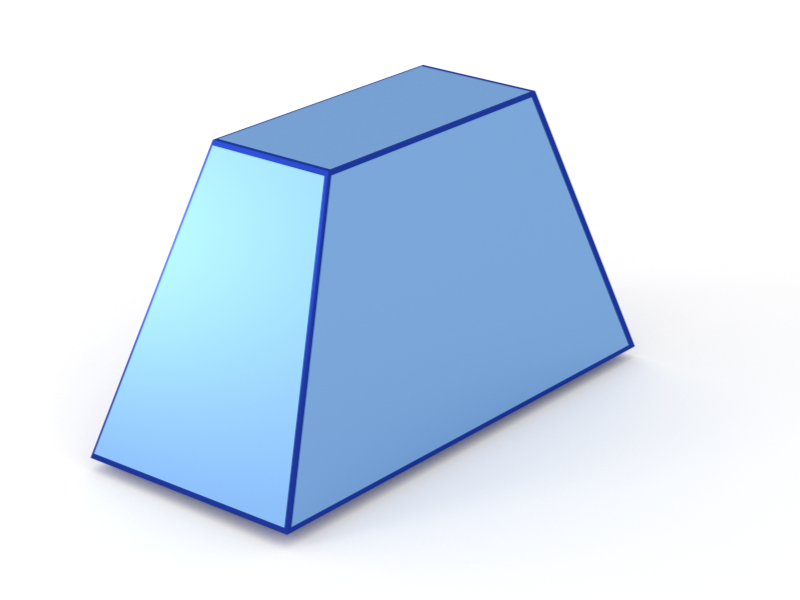
\includegraphics[width=.24\textwidth]{fig/blue/AnistropicPyramid3d.png}}
\hfill
\subfigure[Top view]{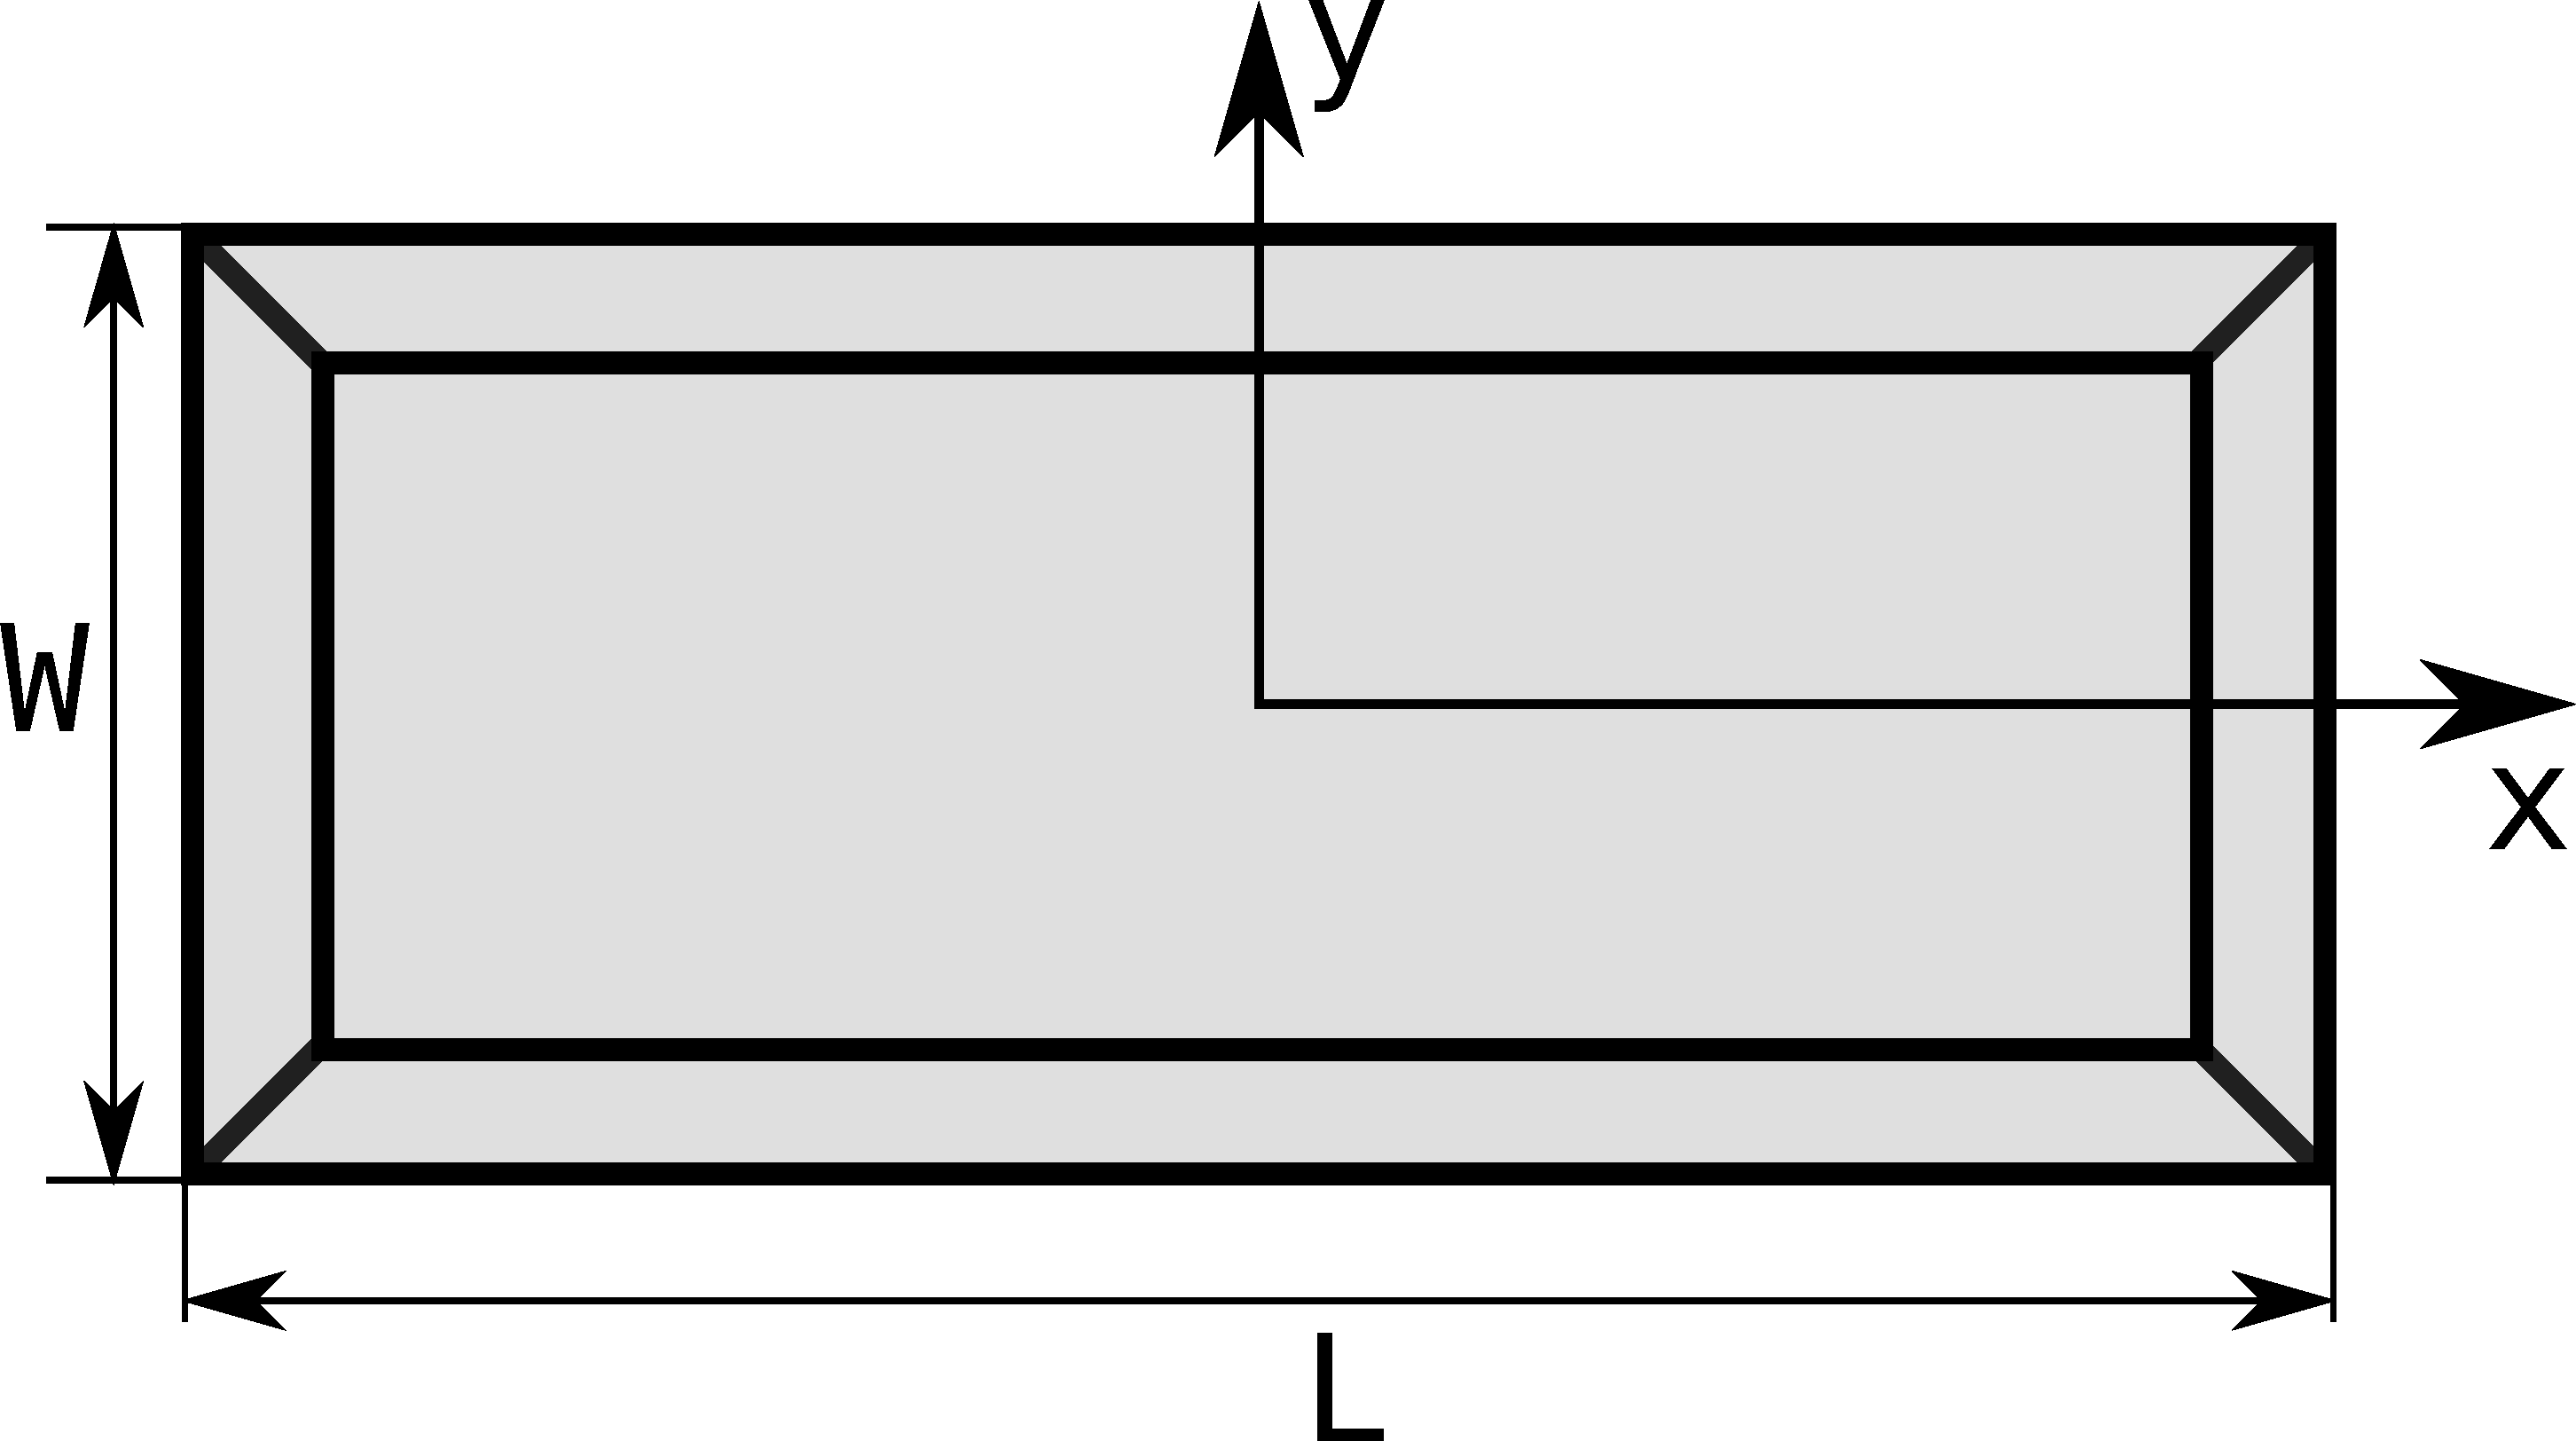
\includegraphics[width=.30\textwidth]{fig/cuts/AnisoPyramid2dxy.pdf}}
\hfill
\subfigure[Side view]{\raisebox{2mm}{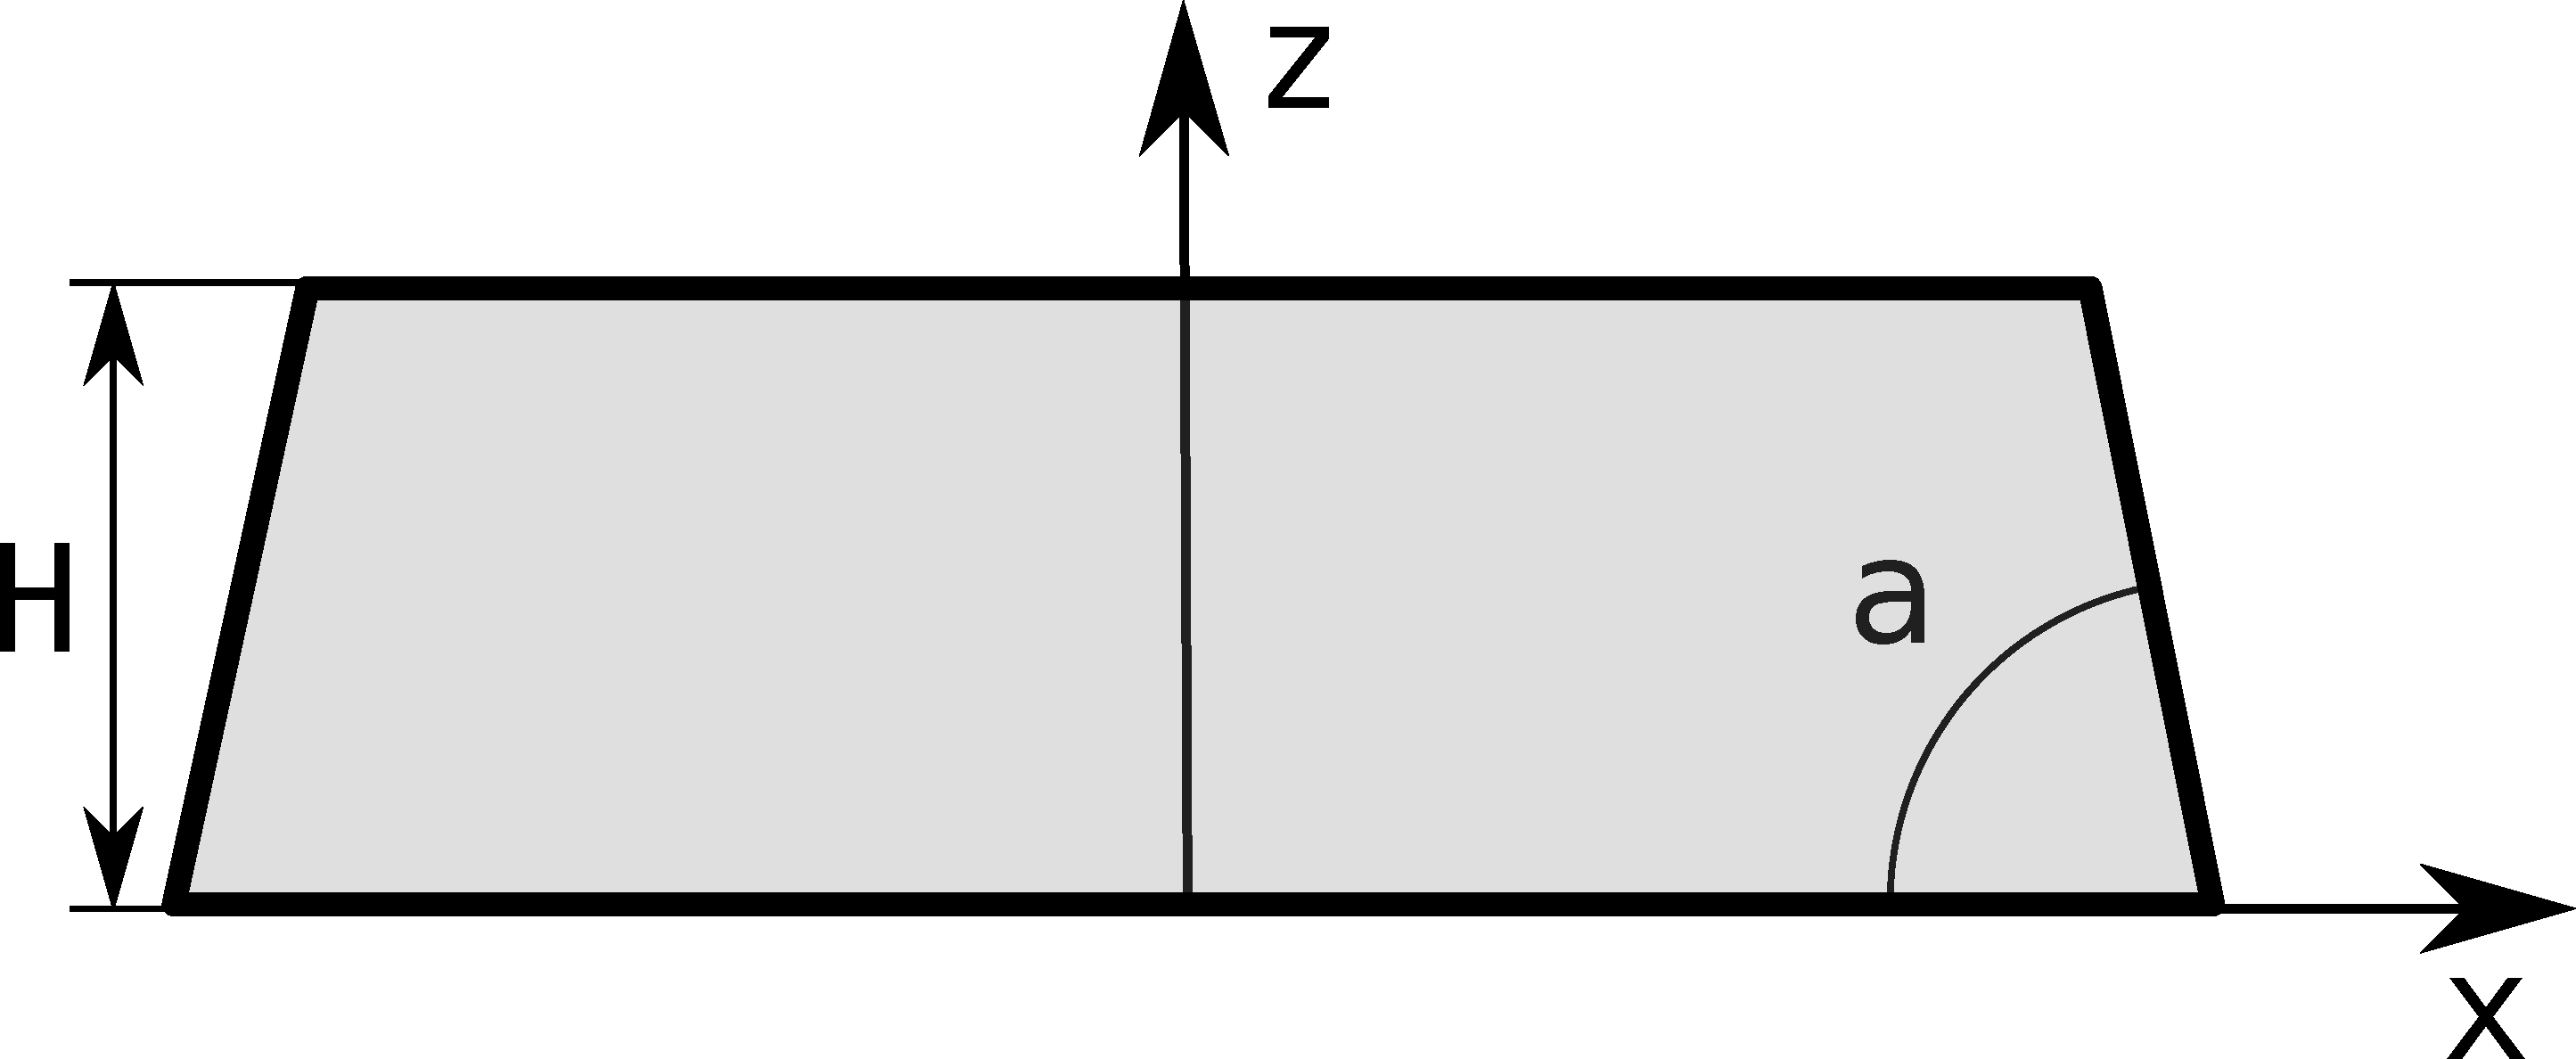
\includegraphics[width=.30\textwidth]{fig/cuts/AnisoPyramid2dxz.pdf}}}
\hfill
\caption{A truncated right pyramid with a rectangular base.}
\end{figure}

\FloatBarrier

\paragraph{Syntax and parameters}\strut\\[-2ex plus .2ex minus .2ex]
\begin{lstlisting}[language=python, style=eclipseboxed,numbers=none,nolol]
  FormFactorAnisoPyramid(length, width, height, alpha)
\end{lstlisting}
with the parameters
\begin{itemize}
\item \texttt{length} of the base, $L$,
\item \texttt{width} of the base, $W$,
\item \texttt{height}, $H$
\item \texttt{alpha}, angle between the base and a side face, $\alpha$.
\end{itemize}
They must fulfill
\begin{displaymath}
  H \le \frac{\tan\alpha}{2} L
  \quad\text{and}\quad
  H \le \frac{\tan\alpha}{2} W
\end{displaymath}

\paragraph{Form factor etc}\strut\\
Notation:
\begin{displaymath}
  \ell\coloneqq L/2,\quad
  w\coloneqq W/2,\quad
  h\coloneqq H/2,\quad
  f_\pm(z)\coloneqq \exp(\pm i z)\sinc(z).
\end{displaymath}
Results:
\begin{equation*}
\begin{array}{@{}l@{}l@{}}
\DS F=
\frac{H}{q_xq_y} \Big\{
   &+\DS  f_+\left(\left(\frac{q_x-q_y}{\tan\alpha} +q_z\right)h\right)
        \exp(-i(q_x\ell-q_y w))
\\[3.6ex]
   &\DS+ f_-\left(\left(\frac{q_x-q_y}{\tan\alpha} -q_z\right)h\right)
        \exp(+i(q_x\ell-q_y w))
\\[3.6ex]
   &\DS- f_+\left(\left(\frac{q_x+q_y}{\tan\alpha} +q_z\right)h\right)
        \exp(-i(q_x\ell+q_y w))
\\[3.6ex]
   &\DS- f_-\left(\left(\frac{q_x+q_y}{\tan\alpha} -q_z\right)h\right)
        \exp(+i(q_x\ell+q_y w))
\Big\},
\end{array}
\end{equation*}
\begin{equation*}
  V= H \Big[LW - \dfrac{(L + W)H}{\tan\alpha} + \dfrac{4}{3} \dfrac{H^2}{\tan^2\alpha}\Big].
\end{equation*}
\begin{equation*}
  S=LW.
\end{equation*}

\paragraph{Example}\strut\\
Figure~\ref{fig:FFAnisoPyramidEx} shows the normalized intensity
$|F|^2/V^2$, computed with $L=20$~nm, $W=16$~nm, $H=13$~nm, and
$\alpha=60^{\circ}$.

\begin{figure}[H]
\begin{center}
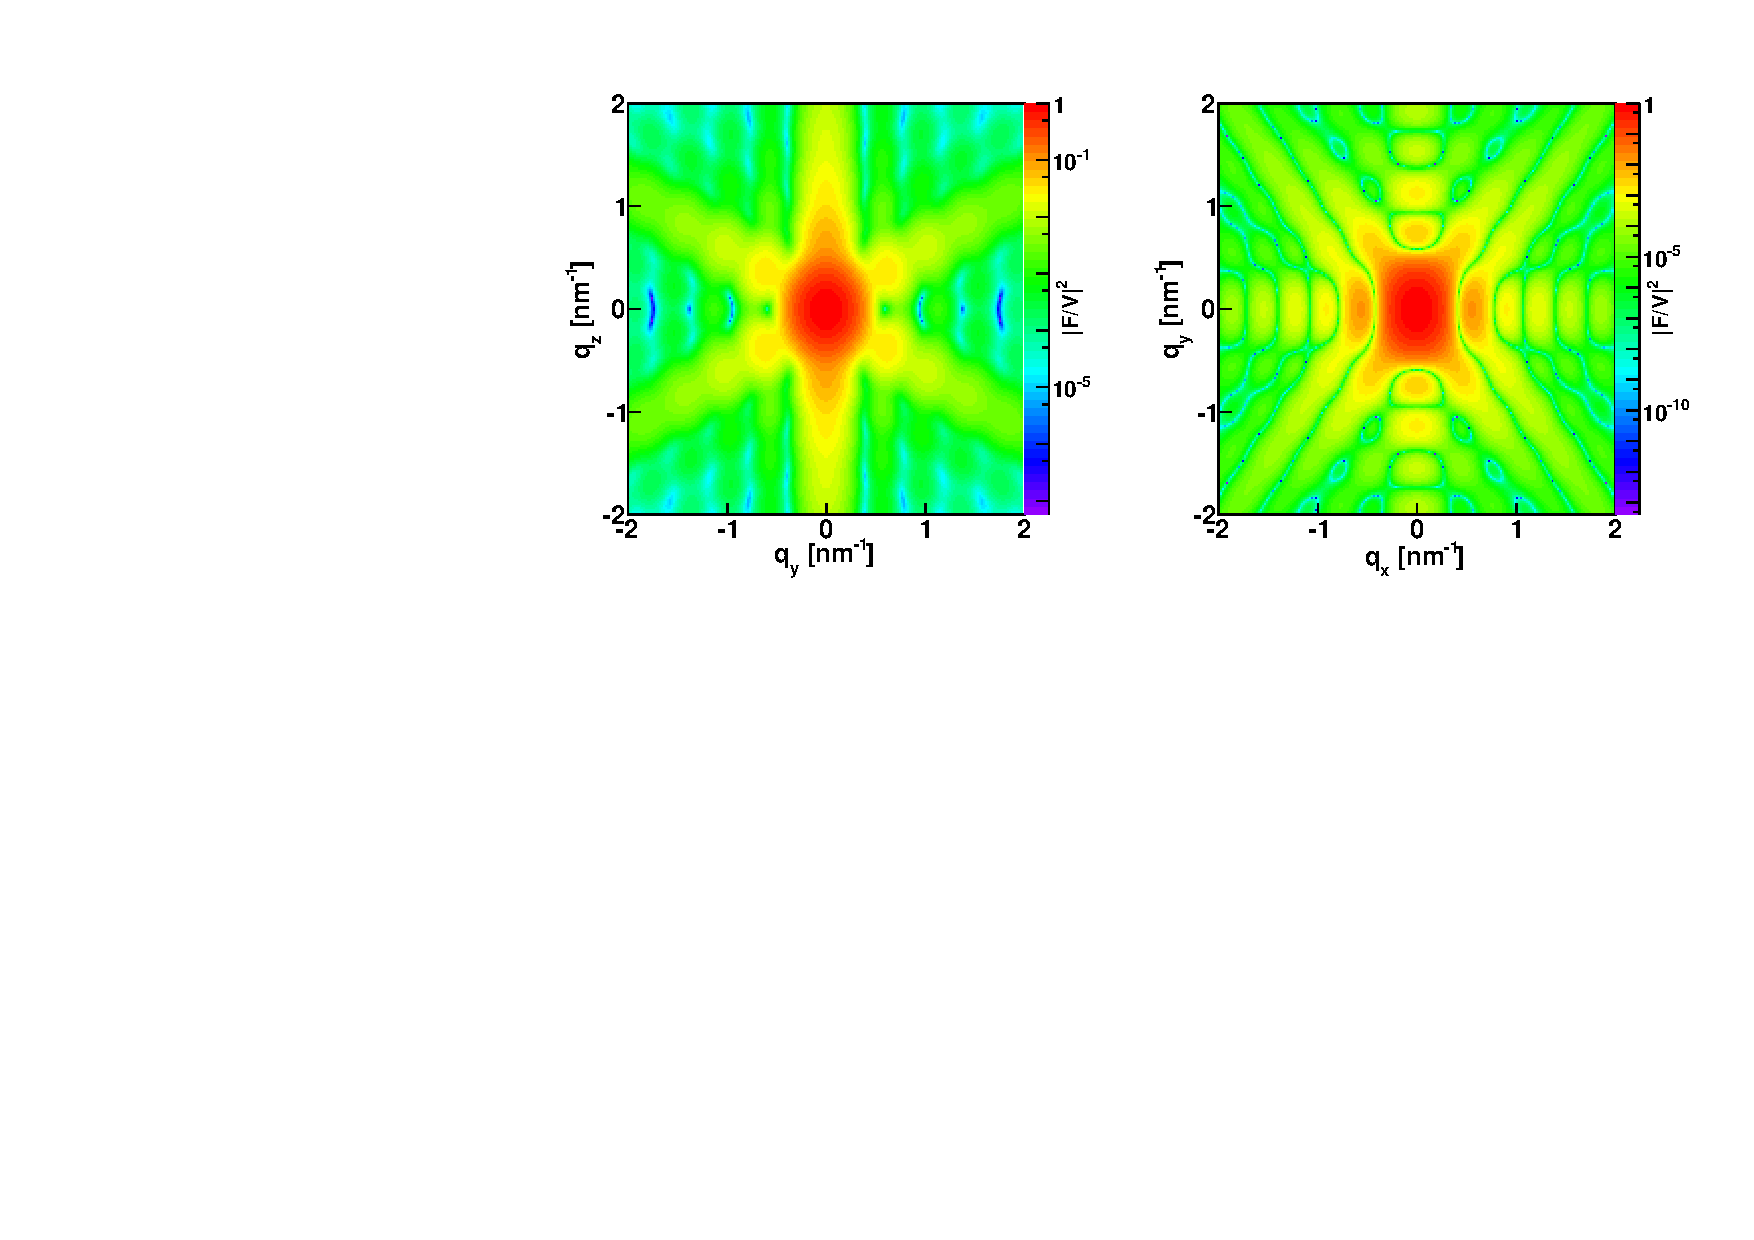
\includegraphics[angle=-90,width=\textwidth]{fig/ff/figffanisopyramid.pdf}
\end{center}
\caption{Normalized intensity for the form factor of an anisotropic
  pyramid $|F|^2/V^2$, plotted against ($q_y$, $q_z$) and  ($q_x$, $q_y$) and computed with \Code{FormFactorAnisoPyramid(20.*nanometer, 16.*nanometer, 13.*nanometer, 60.*degree)}.}
\label{fig:FFAnisoPyramidEx}
\end{figure}

\paragraph{References}\strut\\
Agrees with the \E{In-plane anisotropic pyramid} form factor of \IsGISAXS\
\cite[Eq.~2.40]{Laz08} \cite[Eq.~217]{ReLL09},
except for different parametrization and
for a refactoring of the analytical expression for $F(\q)$.

%-------------------------------------------------------------------------------
\FloatBarrier\newpage
\subsection{Box (cuboid)} \label{sec:Box}
  \index{Box (form factor)}
  \index{Cuboid (form factor)}
  \index{Prism (form factor)!reactangular (Box)}
  \index{FormFactorBox@\Code{FormFactorBox}}
%-------------------------------------------------------------------------------

\paragraph{Real-space geometry}\strut\\

\begin{figure}[H]
\hfill
\subfigure[Perspective]{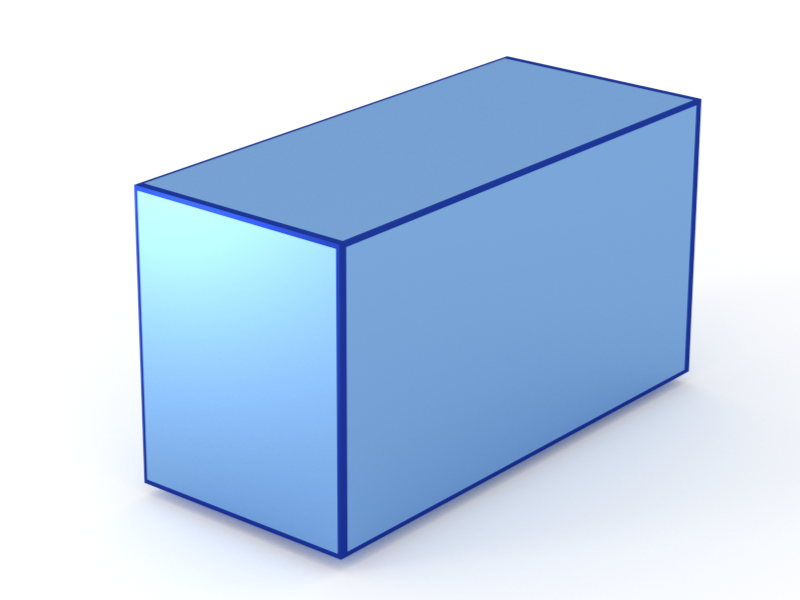
\includegraphics[width=.24\textwidth]{fig/blue/Box3d.png}}
\hfill
\subfigure[Top view]{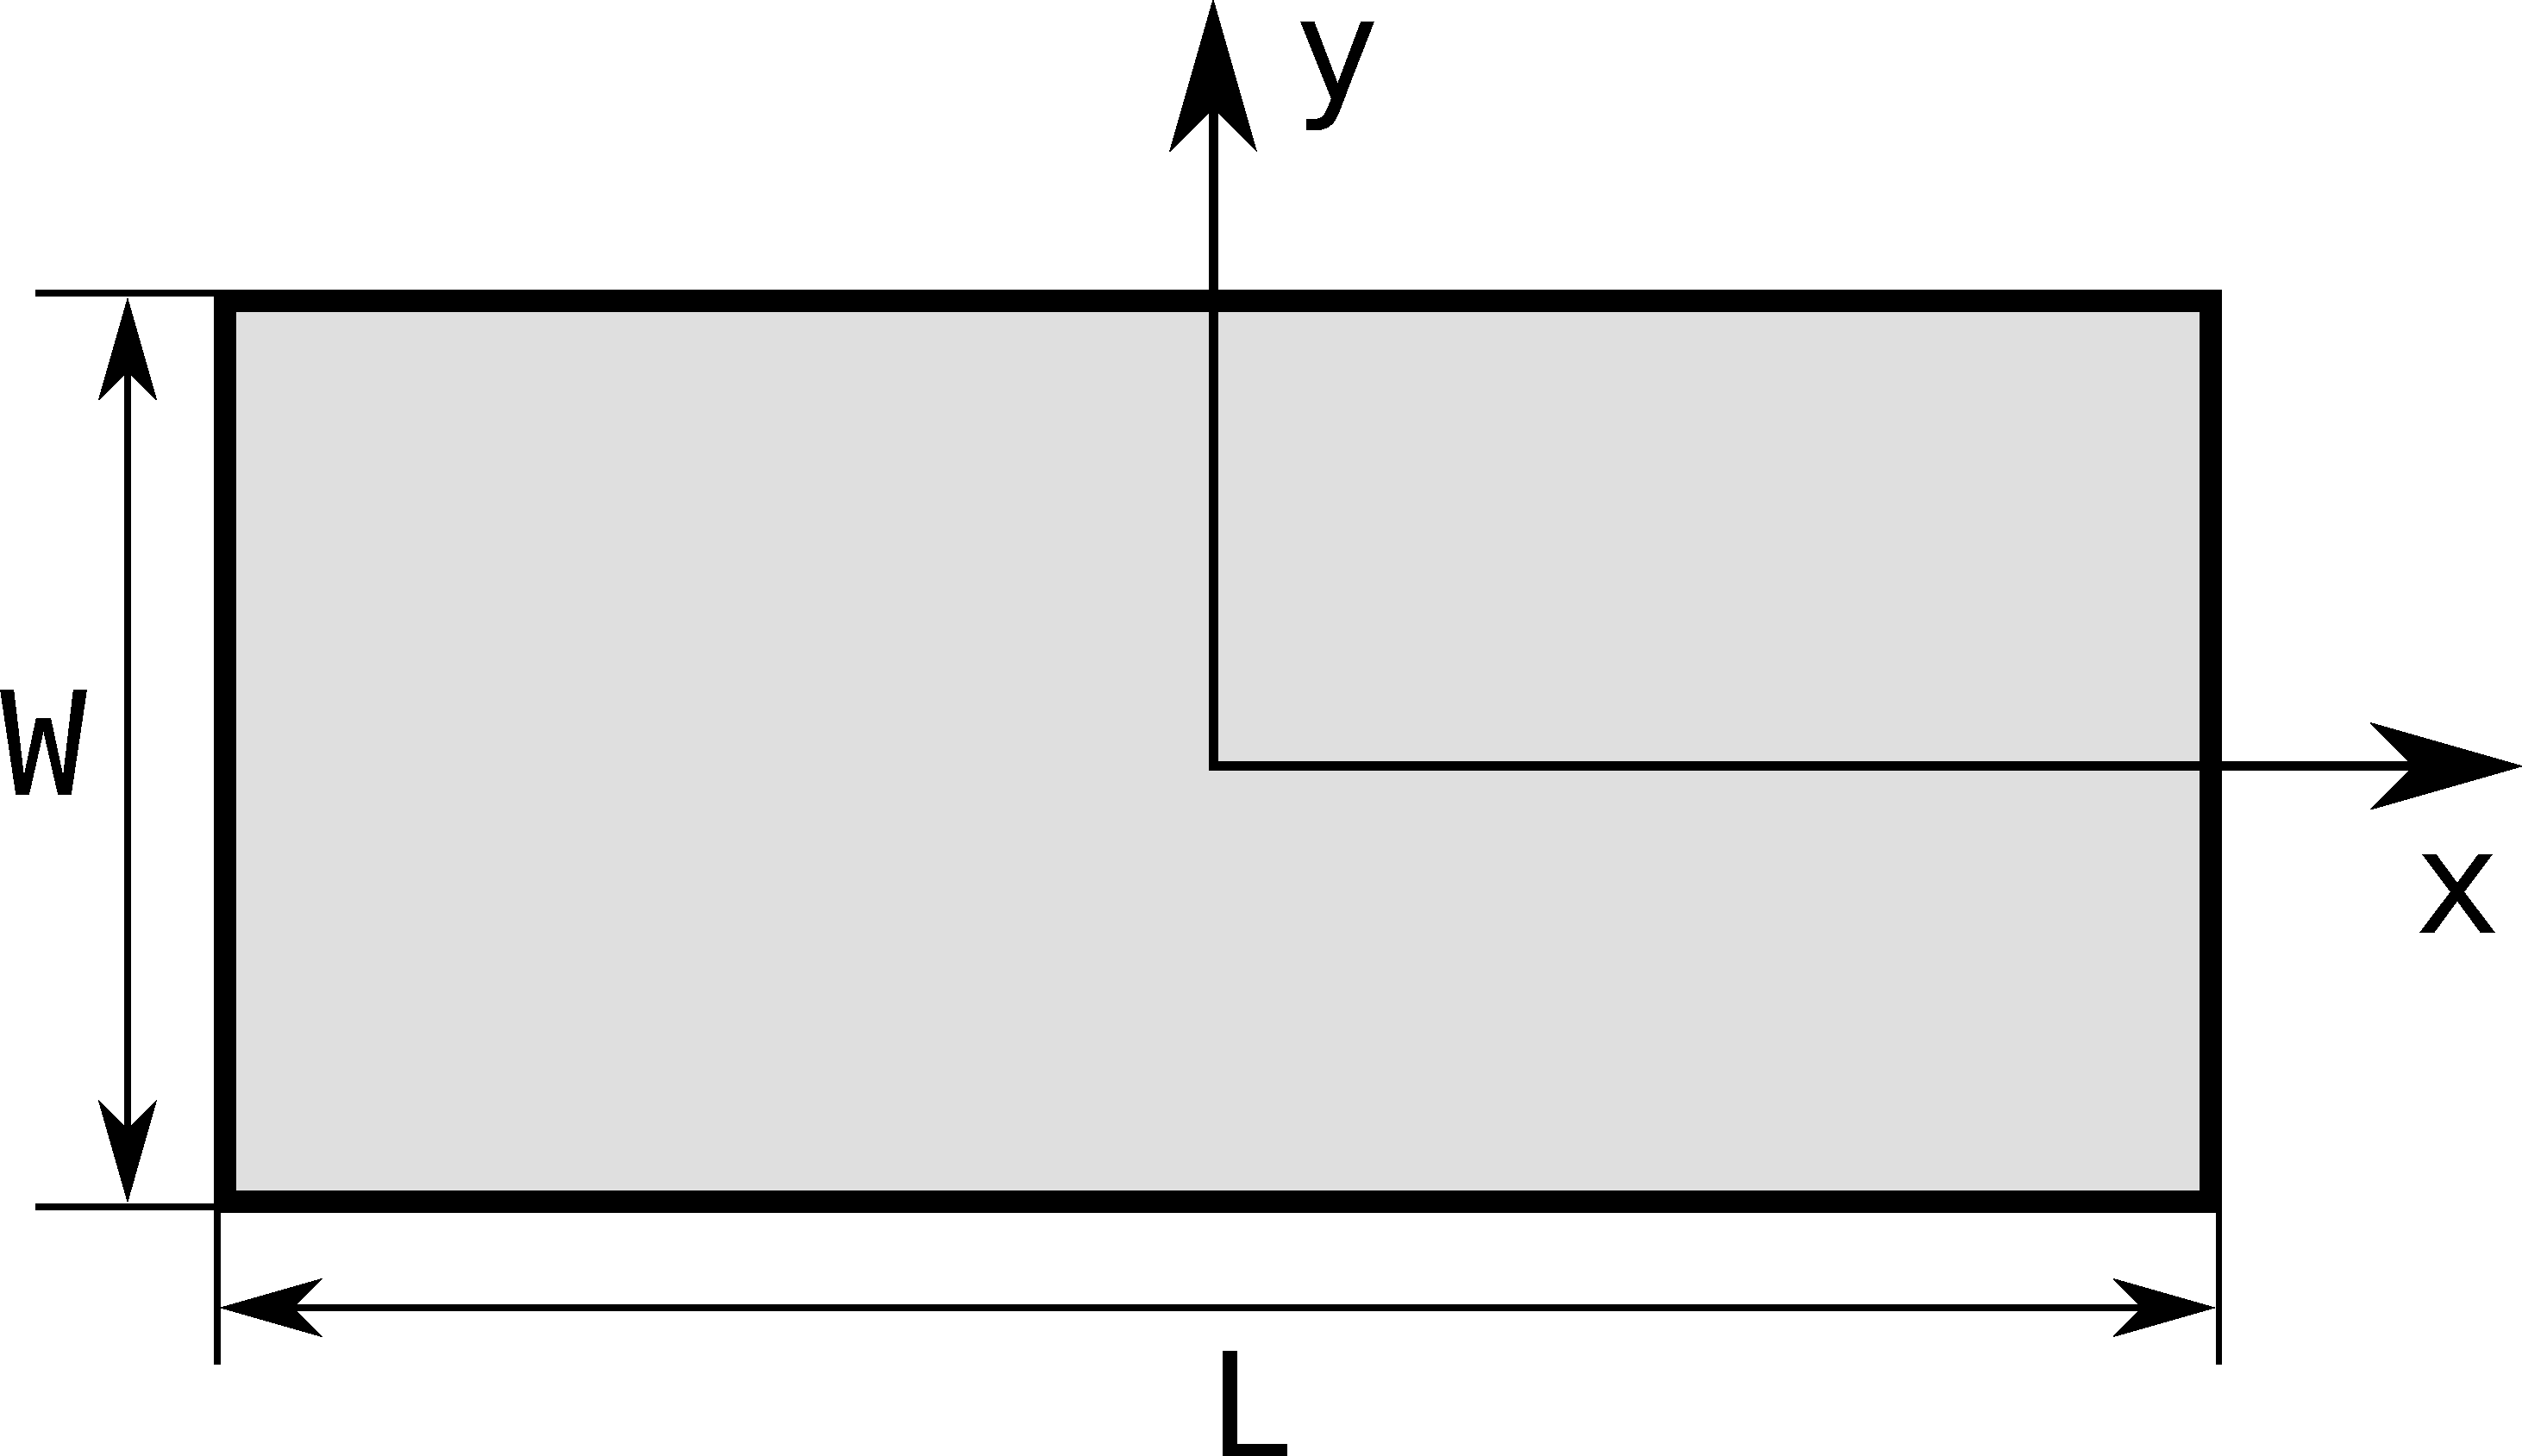
\includegraphics[width=.30\textwidth]{fig/cuts/Box2dxy.pdf}}
\hfill
\subfigure[Side view]{\raisebox{2mm}{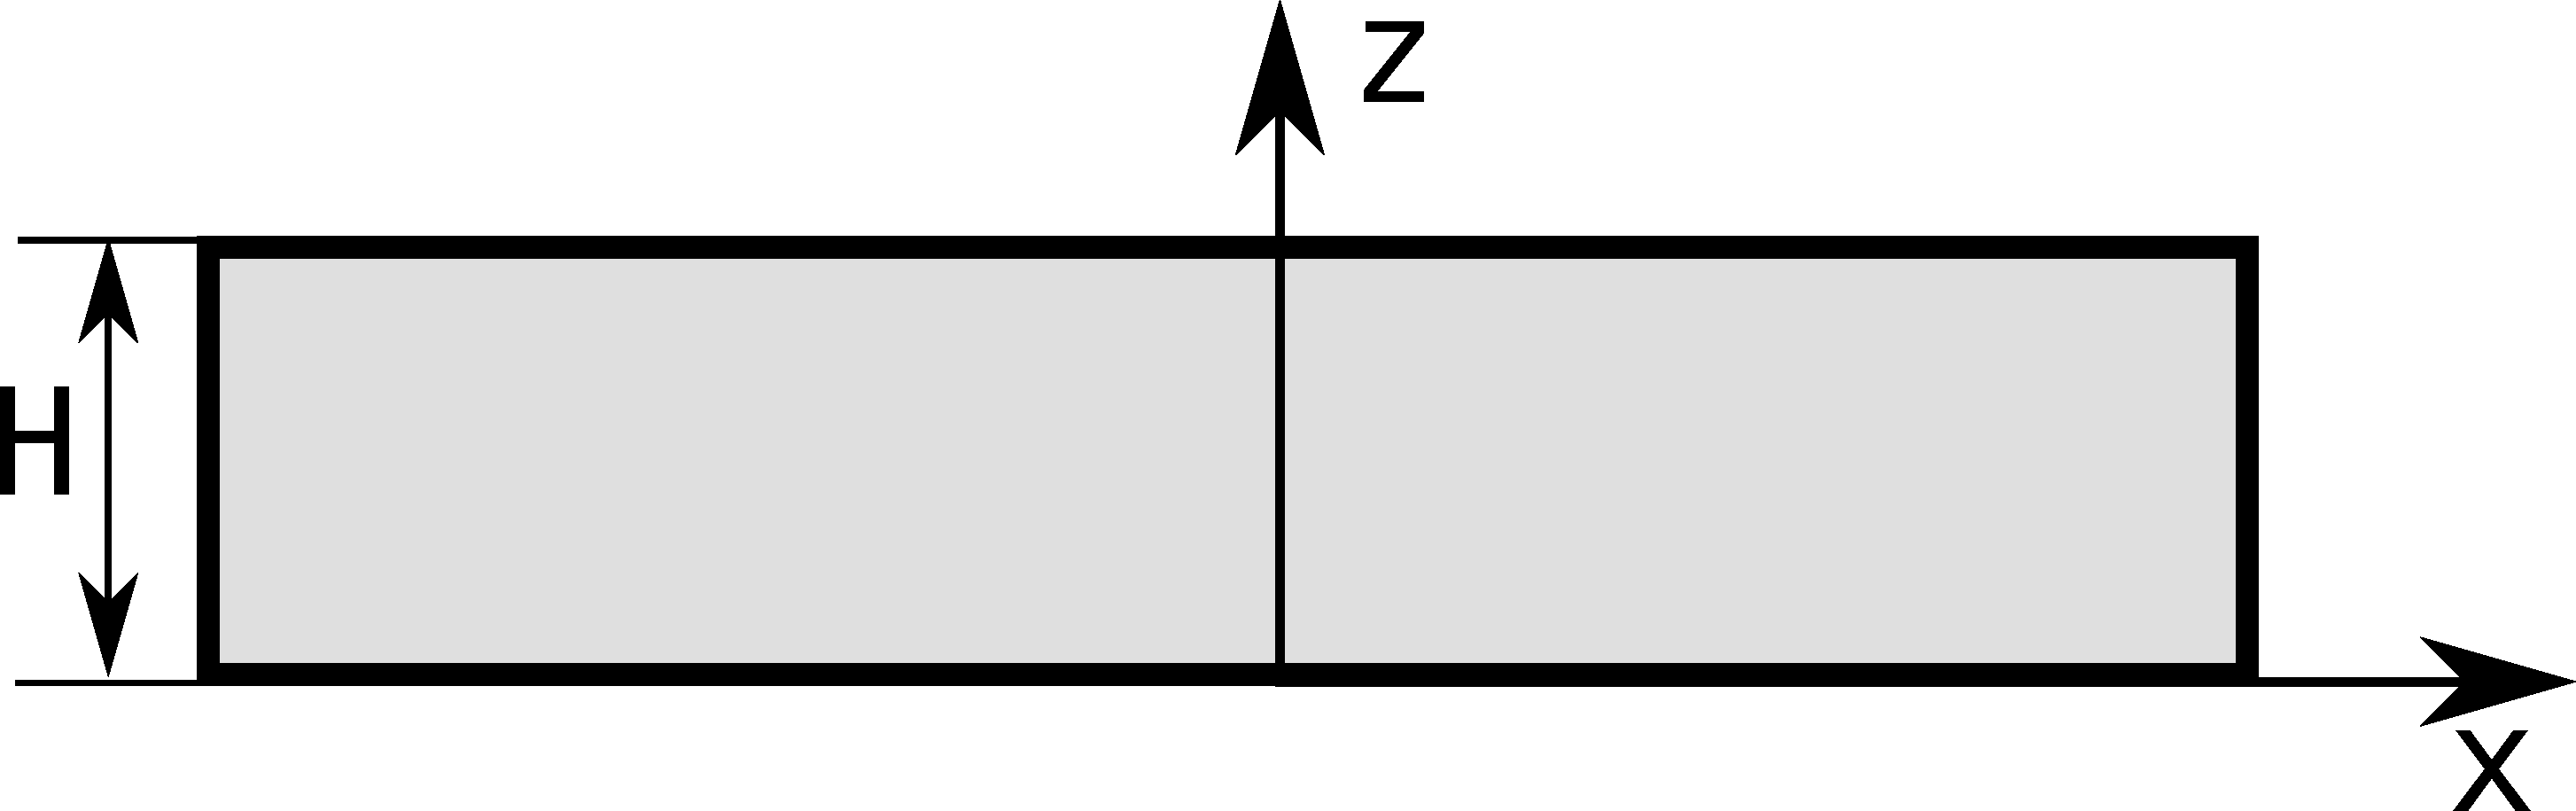
\includegraphics[width=.30\textwidth]{fig/cuts/Box2dxz.pdf}}}
\hfill
\caption{A rectangular cuboid.}
\end{figure}

\FloatBarrier

\paragraph{Syntax and parameters}\strut\\[-2ex plus .2ex minus .2ex]
\begin{lstlisting}[language=python, style=eclipseboxed,numbers=none,nolol]
  FormFactorBox(length, width, height)
\end{lstlisting}
with the parameters
\begin{itemize}
\item \texttt{length} of the base, $L$,
\item \texttt{width} of the base, $W$,
\item \texttt{height}, $H$.
\end{itemize}


\paragraph{Form factor etc}

\begin{equation*}
F= L W H\exp\left(i q_z \frac{H}{2}\right) \sinc\left(q_x \frac{L}{2}\right)
\sinc\left(q_y \frac{W}{2}\right) \sinc\left(q_z \frac{H}{2}\right),
\end{equation*}
\begin{equation*}
  V= LWH,
\end{equation*}
\begin{equation*}
  S = LW.
\end{equation*}

\paragraph{Example}\strut\\
Figure~\ref{fig:FFBoxEx} shows the normalized intensity
$|F|^2/V^2$, computed with $L=20$~nm, $W=16$~nm, and $H=13$~nm:

\begin{figure}[H]
\begin{center}
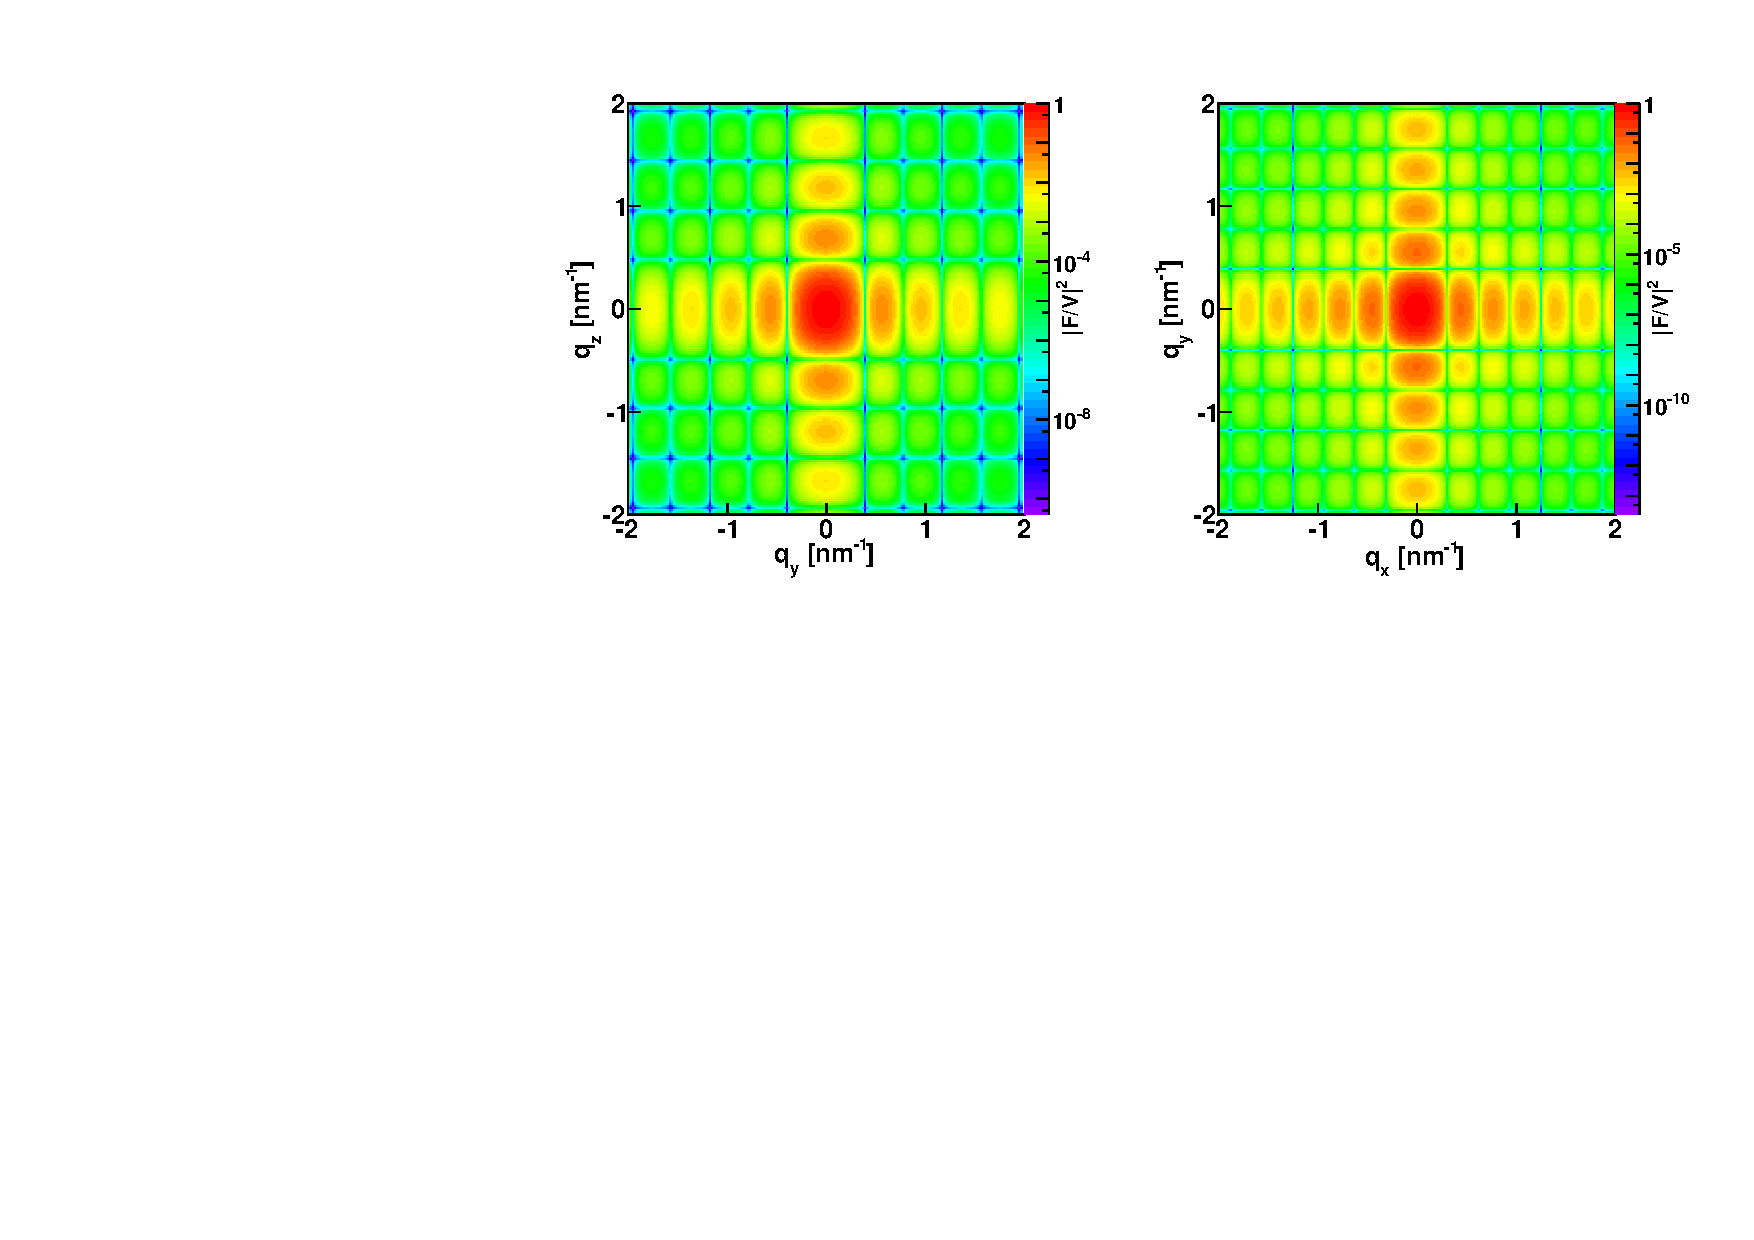
\includegraphics[angle=-90,width=\textwidth]{fig/ff/figffbox.pdf}
\end{center}
\caption{Normalized intensity for the form factor of a Box plotted against ($q_y$, $q_z$) and  ($q_x$, $q_y$) and computed with \Code{FormFactorBox(20.*nanometer, 16.*nanometer, 13.*nanometer)}.}
\label{fig:FFBoxEx}
\end{figure}

\paragraph{References}\strut\\
Agrees with \E{Box} form factor of \IsGISAXS\
\cite[Eq.~2.38]{Laz08} \cite[Eq.~214]{ReLL09},
except for factors $1/2$ in the definitions of parameters $L$, $W$, $H$.

%-------------------------------------------------------------------------------
\clearpage
\subsection{Cone (circular)} \label{sec:Cone} 
  \index{Cone (form factor)!circular}
  \index{Truncated cone (form factor)}
  \index{FormFactorCone@\Code{FormFactorCone}}
%-------------------------------------------------------------------------------

\paragraph{Real-space geometry}

\begin{figure}[H]
\hfill
\subfigure[Perspective]{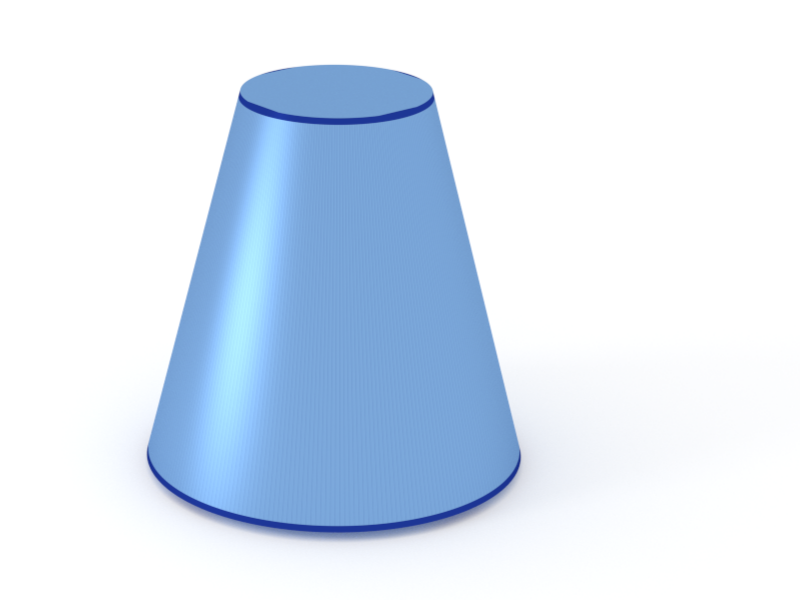
\includegraphics[width=.24\textwidth]{fig/blue/Cone3d.png}}
\hfill
\subfigure[Top view]{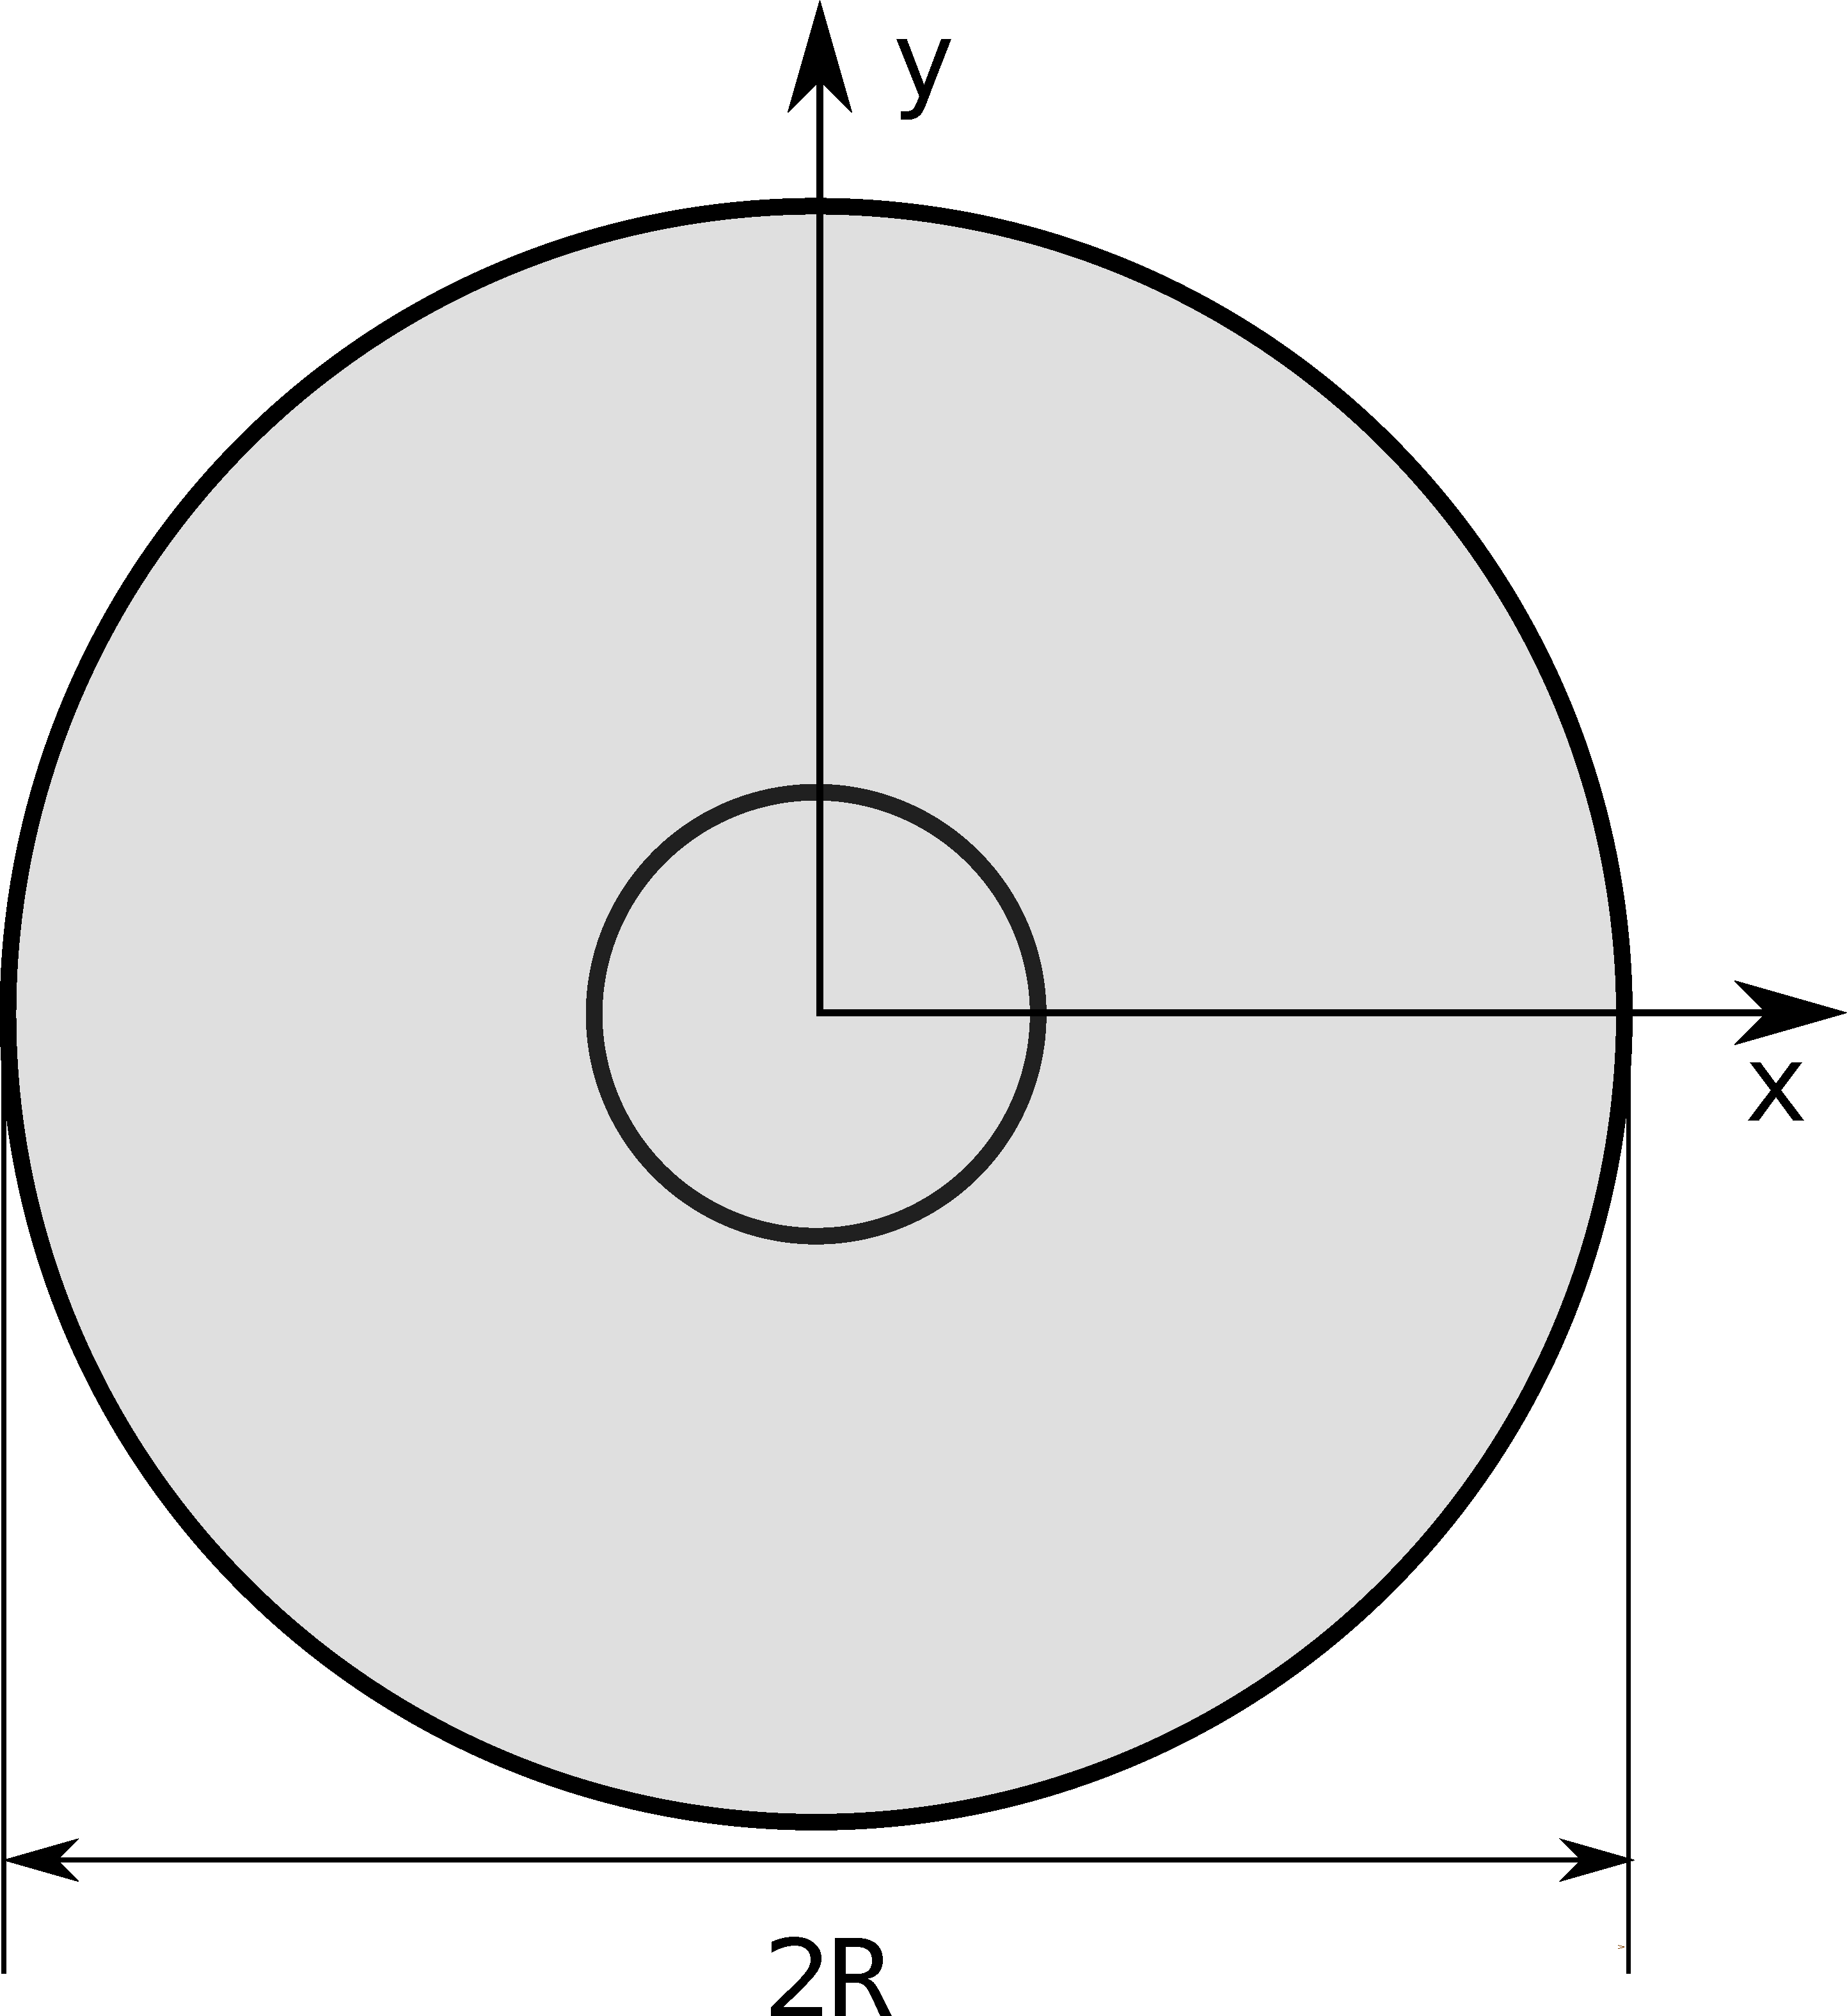
\includegraphics[width=.30\textwidth]{fig/cuts/Cone2dxy.pdf}}
\hfill
\subfigure[Side view]{\raisebox{3mm}{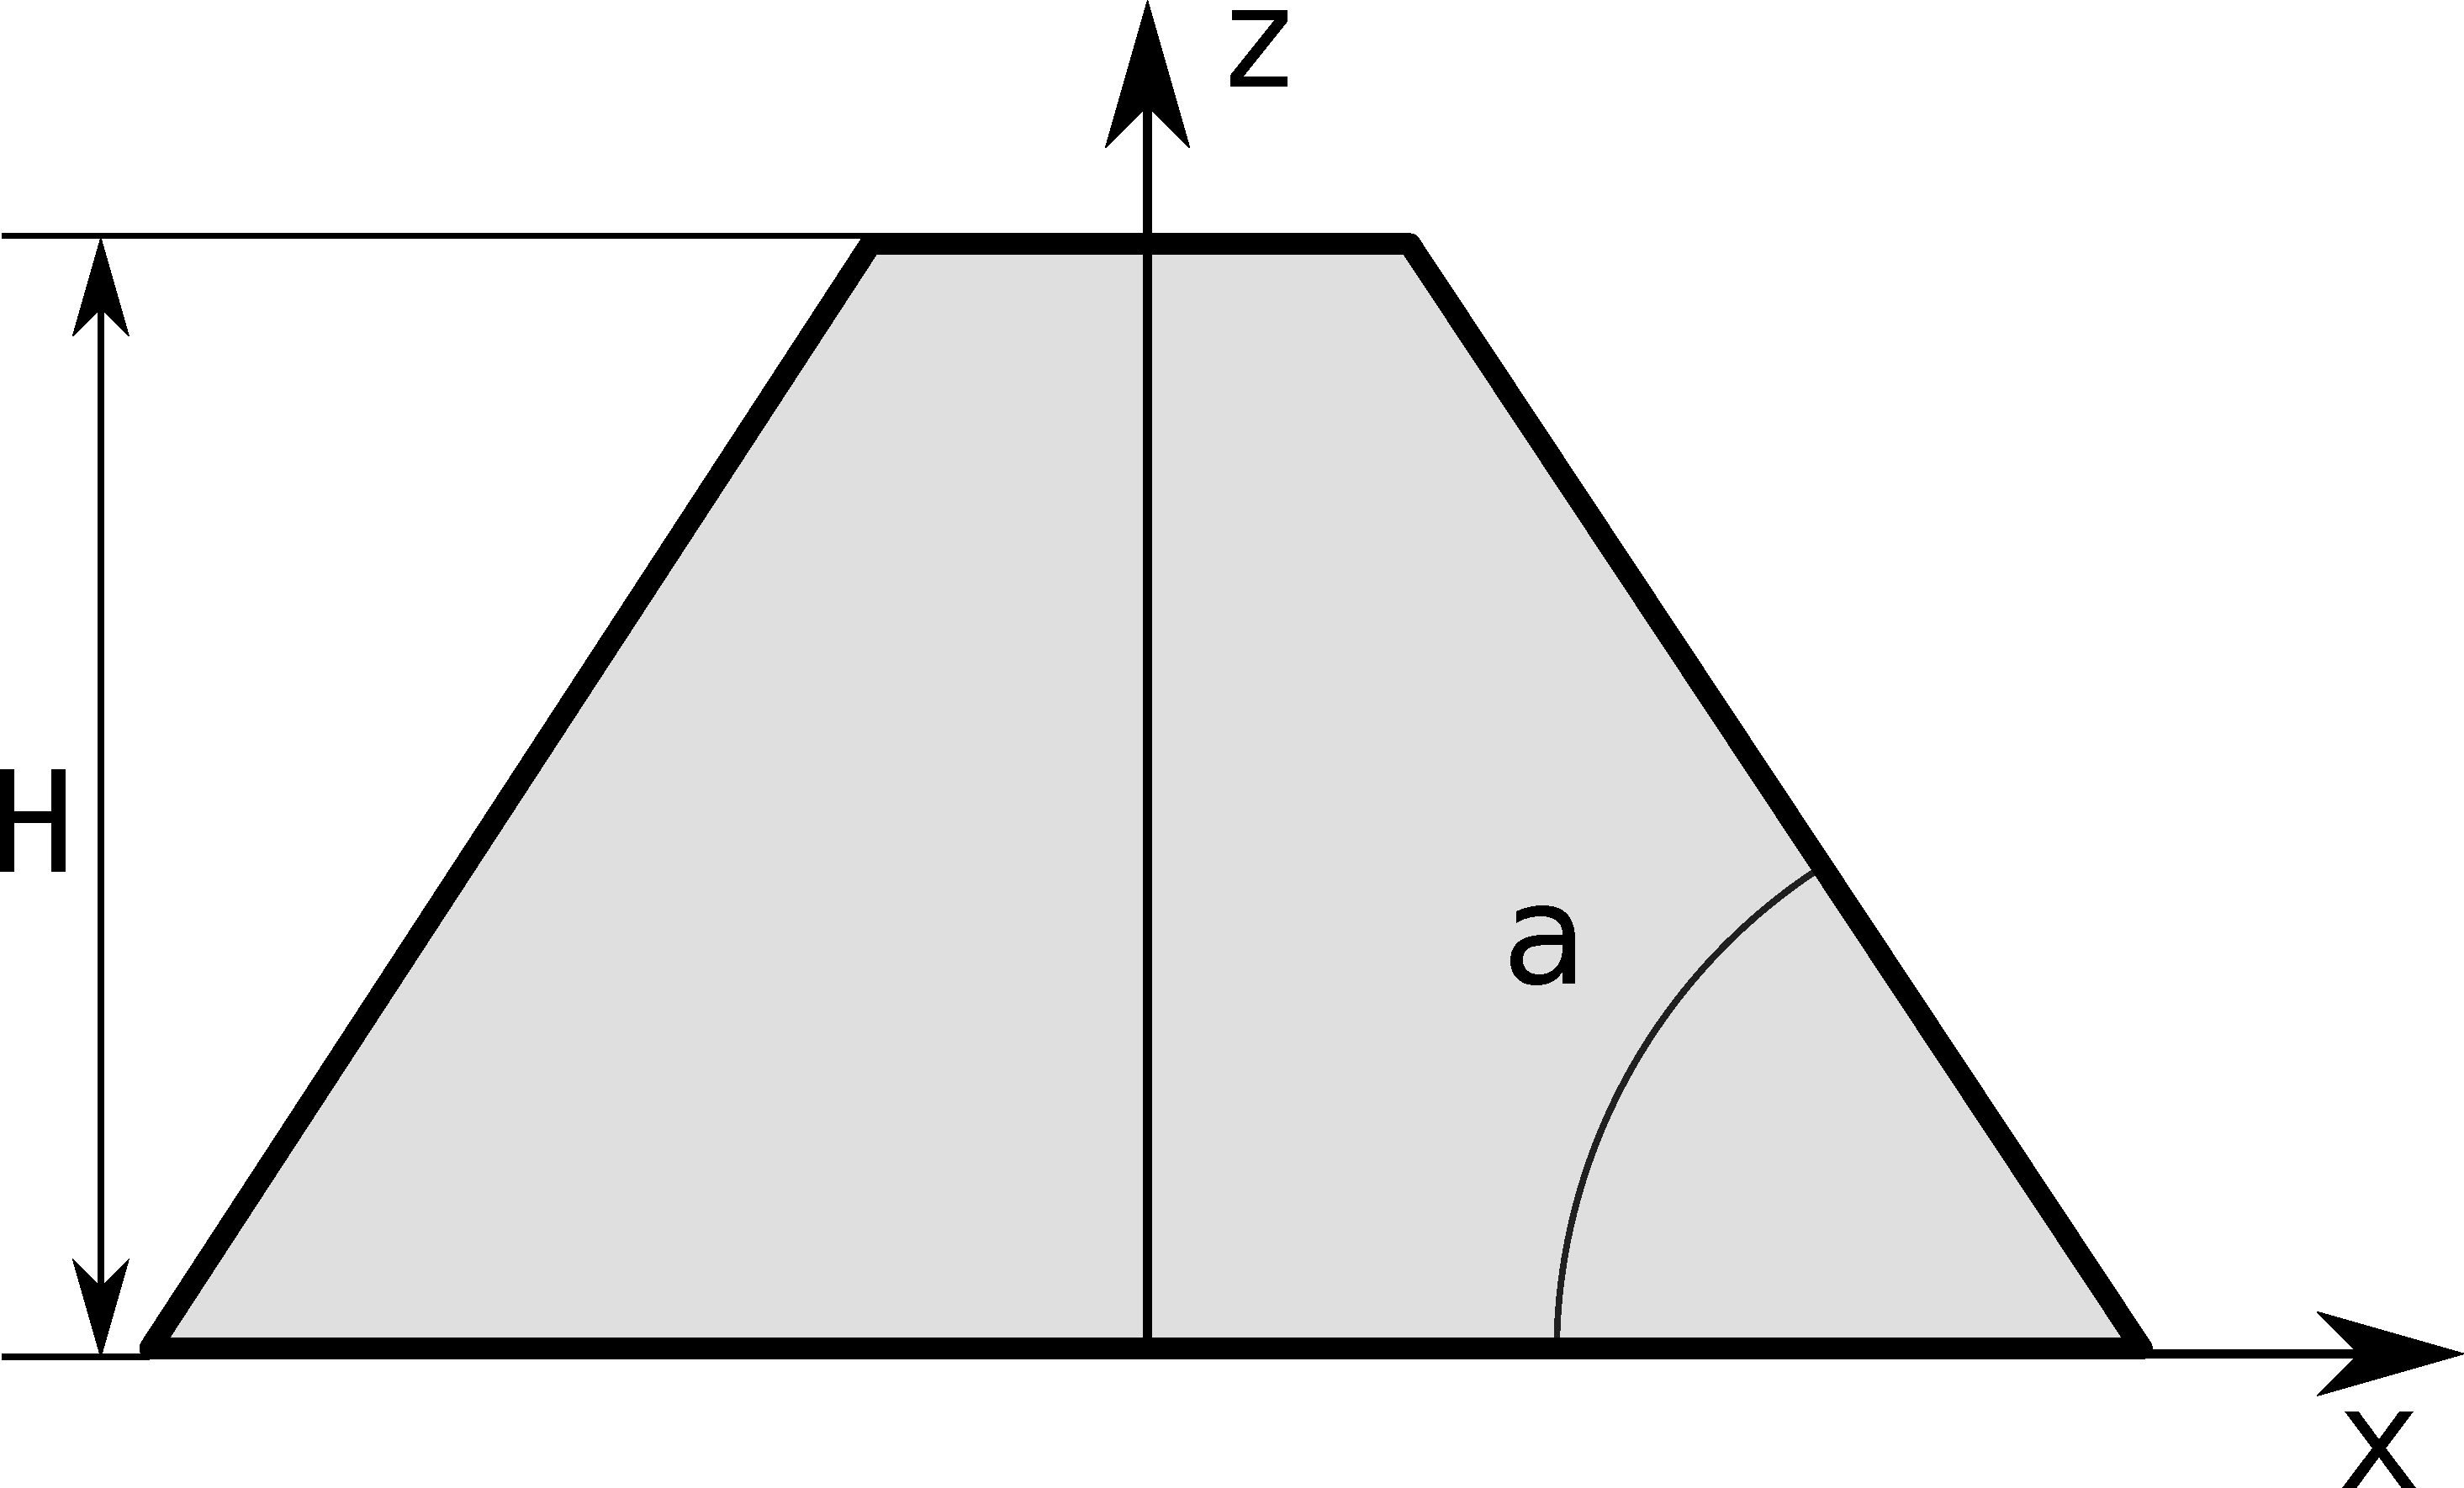
\includegraphics[width=.30\textwidth]{fig/cuts/Cone2dxz.pdf}}}
\hfill
\caption{A truncated cone with circular base.}
\end{figure}

\paragraph{Syntax and parameters}\strut\\[-2ex plus .2ex minus .2ex]
\begin{lstlisting}[language=python, style=eclipseboxed,numbers=none,nolol]
  FormFactorCone(radius, height, alpha)
\end{lstlisting}
with the parameters
\begin{itemize}
\item \texttt{radius}, $R$,
\item \texttt{height}, $H$,
\item \texttt{alpha}, angle between the side and the base, $\alpha$.
\end{itemize}
They must fulfill
\begin{displaymath}
  H\le R\tan\alpha.
\end{displaymath}


\paragraph{Form factor etc}\strut\\
Notation:
\begin{equation*}
  R_H \coloneqq R-\dfrac{H}{\tan \alpha}, \quad
  q_{\parallel} \coloneqq \sqrt{q_x^2+ q_y^2}, \quad
  \tilde{q}_z \coloneqq q_z \tan\alpha.
\end{equation*}
Results:
\begin{equation*}
  F = 2\pi \tan\alpha\; \e^{i\tilde{q}_z R}
      \int_{R_H}^R \!\d\rho\, \rho^2
        \frac{J_1(q_{\parallel}\rho)}{q_{\parallel}\rho}\,\e^{-i\tilde{q}_z \rho},
\end{equation*}
\begin{equation*}
  V = \dfrac{\pi}{3}\tan\alpha  \left( R^3 - R_H^3\right),
\end{equation*}
\begin{equation*}
  S=\pi R^2.
\end{equation*}

\paragraph{Example}\strut\\
Figure~\ref{fig:FFConeEx} shows the normalized intensity
$|F|^2/V^2$, computed with $R=10$~nm, $H=13$~nm, and $\alpha=60^{\circ}$.
\begin{figure}[H]
\begin{center}
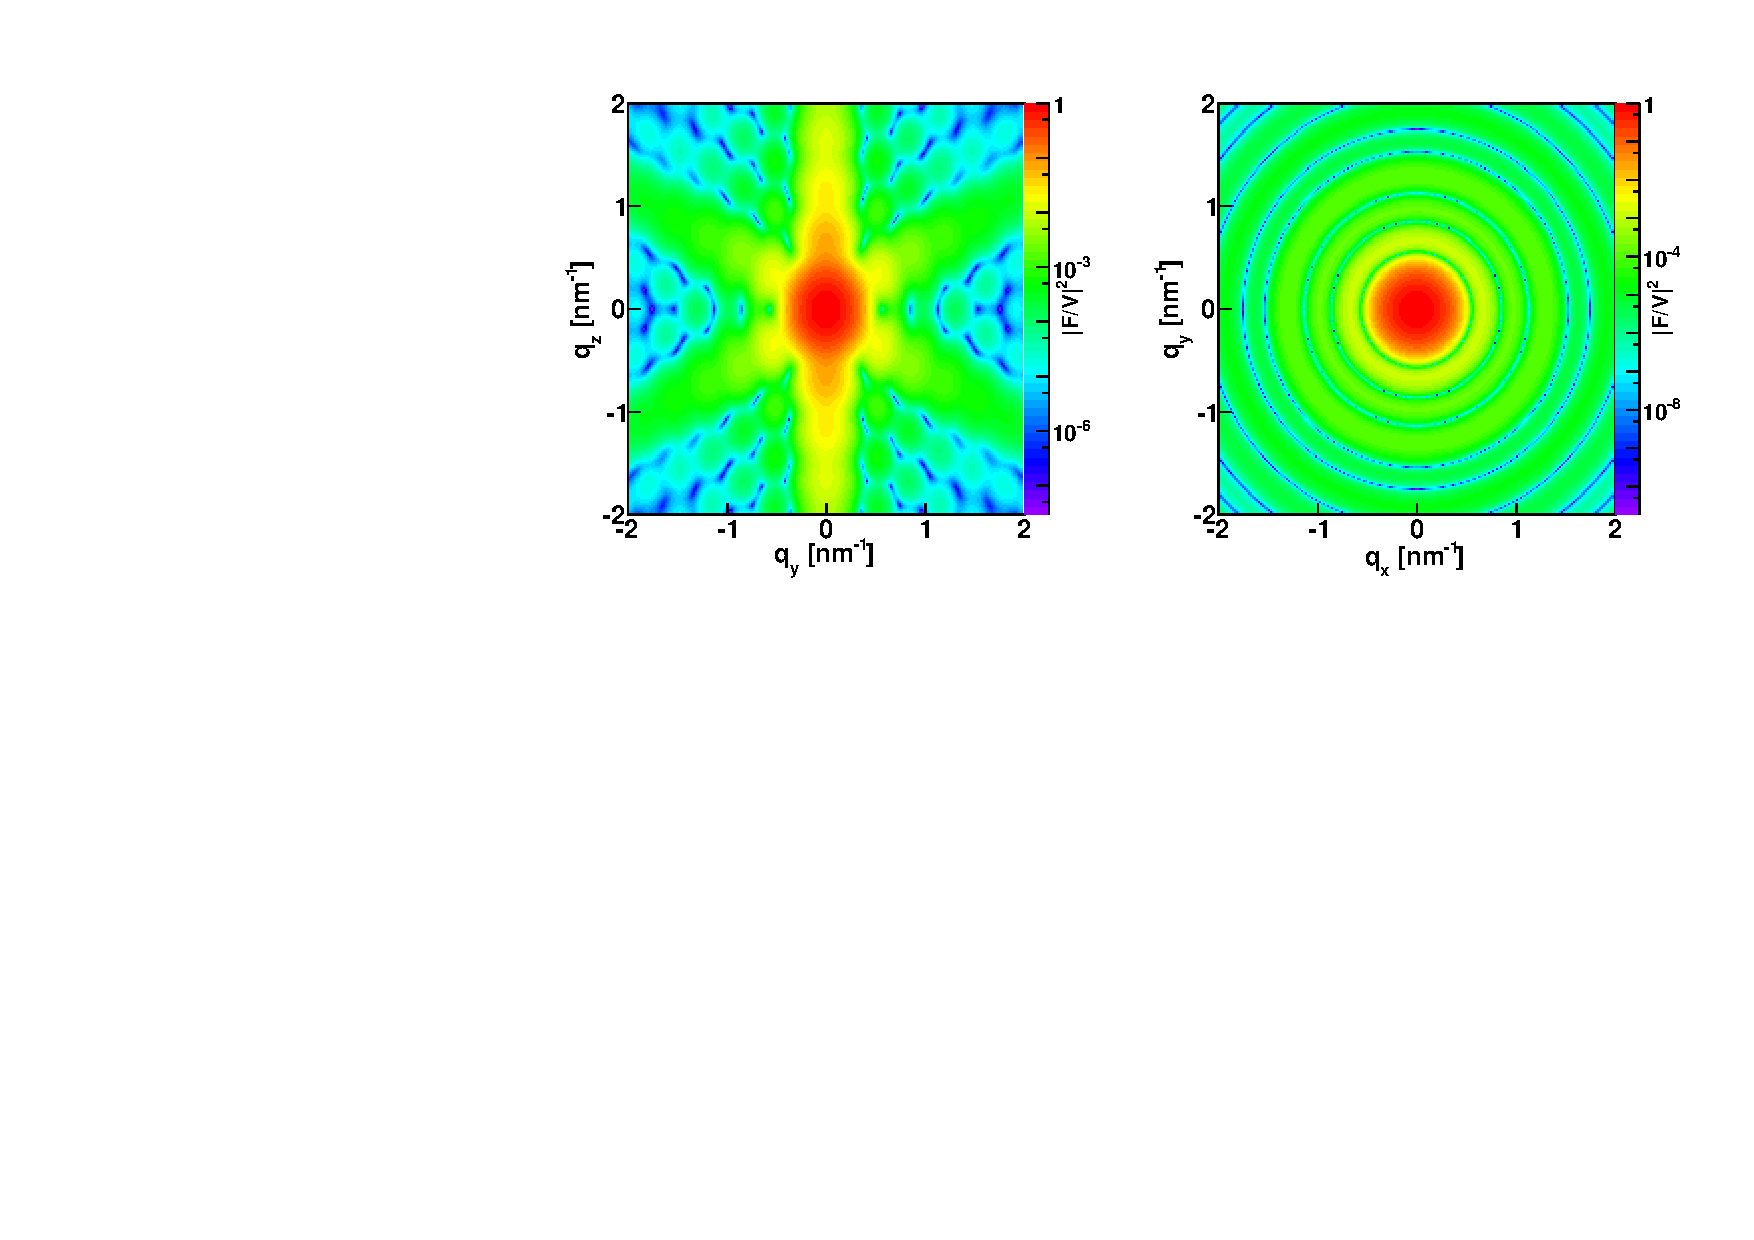
\includegraphics[angle=-90,width=\textwidth]{fig/ff/figffcone.pdf}
\end{center}
\caption{Normalized intensity for the form factor of a Cone plotted against ($q_y$, $q_z$) and ($q_x$, $q_y$.) It
  has been  computed with \Code{FormFactorCone(10.*nanometer,13.*nanometer, 60.*degree)}.}
\label{fig:FFConeEx}
\end{figure}

\paragraph{References}\strut\\
Agrees with \E{Cone} form factor of \IsGISAXS\
\cite[Eq.~2.28]{Laz08} \cite[Eq.~225]{ReLL09},
except for a substitution $z\to\rho$ in our expression for~$F$.


%-------------------------------------------------------------------------------
\clearpage
\subsection{Cone6 (hexagonal)} \label{sec:Cone6}
  \index{Cone (form factor)!hexagonal (Cone6)}
  \index{Pyramid (form factor)!hexagonal (Cone6)}
  \index{Truncated pyramid (form factor)!hexagonal (Cone6)}
  \index{FormFactorCone6@\Code{FormFactorCone6}}
%-------------------------------------------------------------------------------

\paragraph{Real-space geometry}\strut\\

\begin{figure}[H]
\hfill
\subfigure[Perspective]{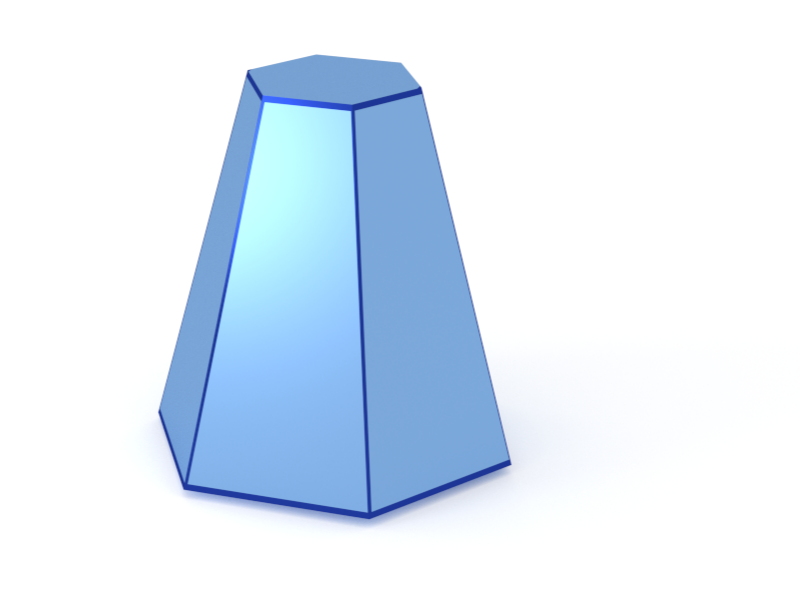
\includegraphics[width=.24\textwidth]{fig/blue/Cone63d.png}}
\hfill
\subfigure[Top view]{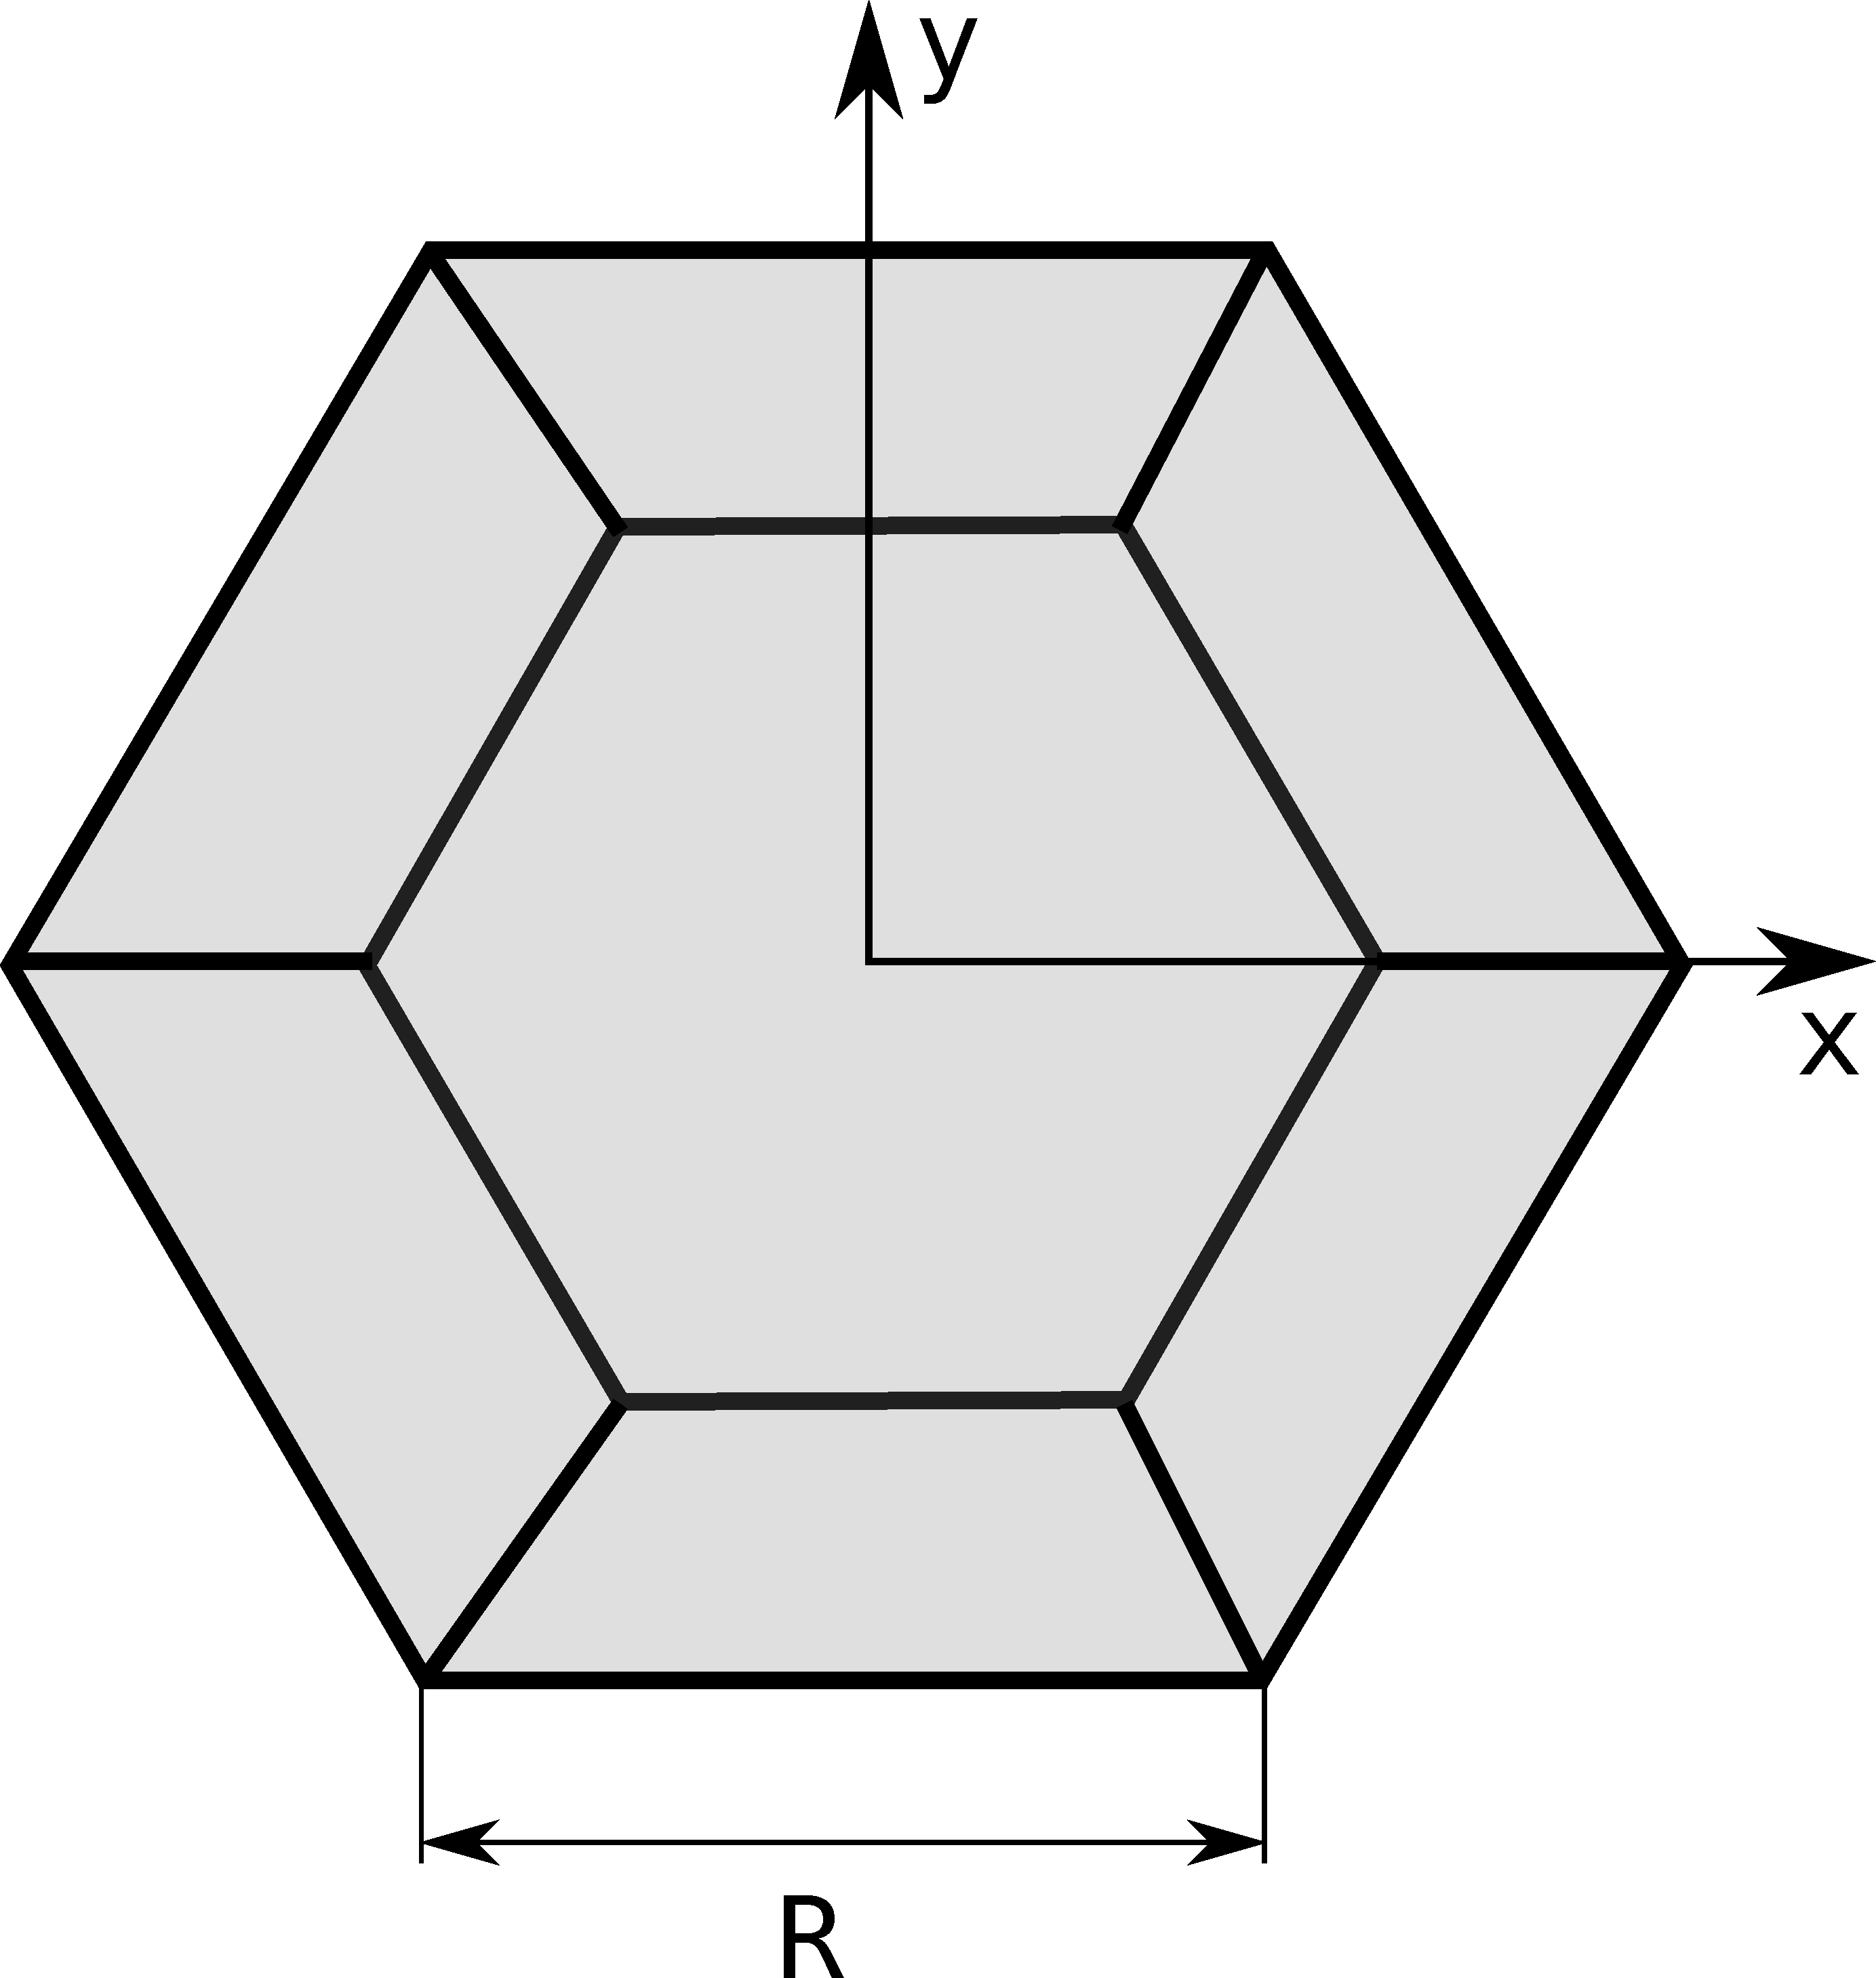
\includegraphics[width=.30\textwidth]{fig/cuts/Cone62dxy.pdf}}
\hfill
\subfigure[Side view]{\raisebox{5mm}{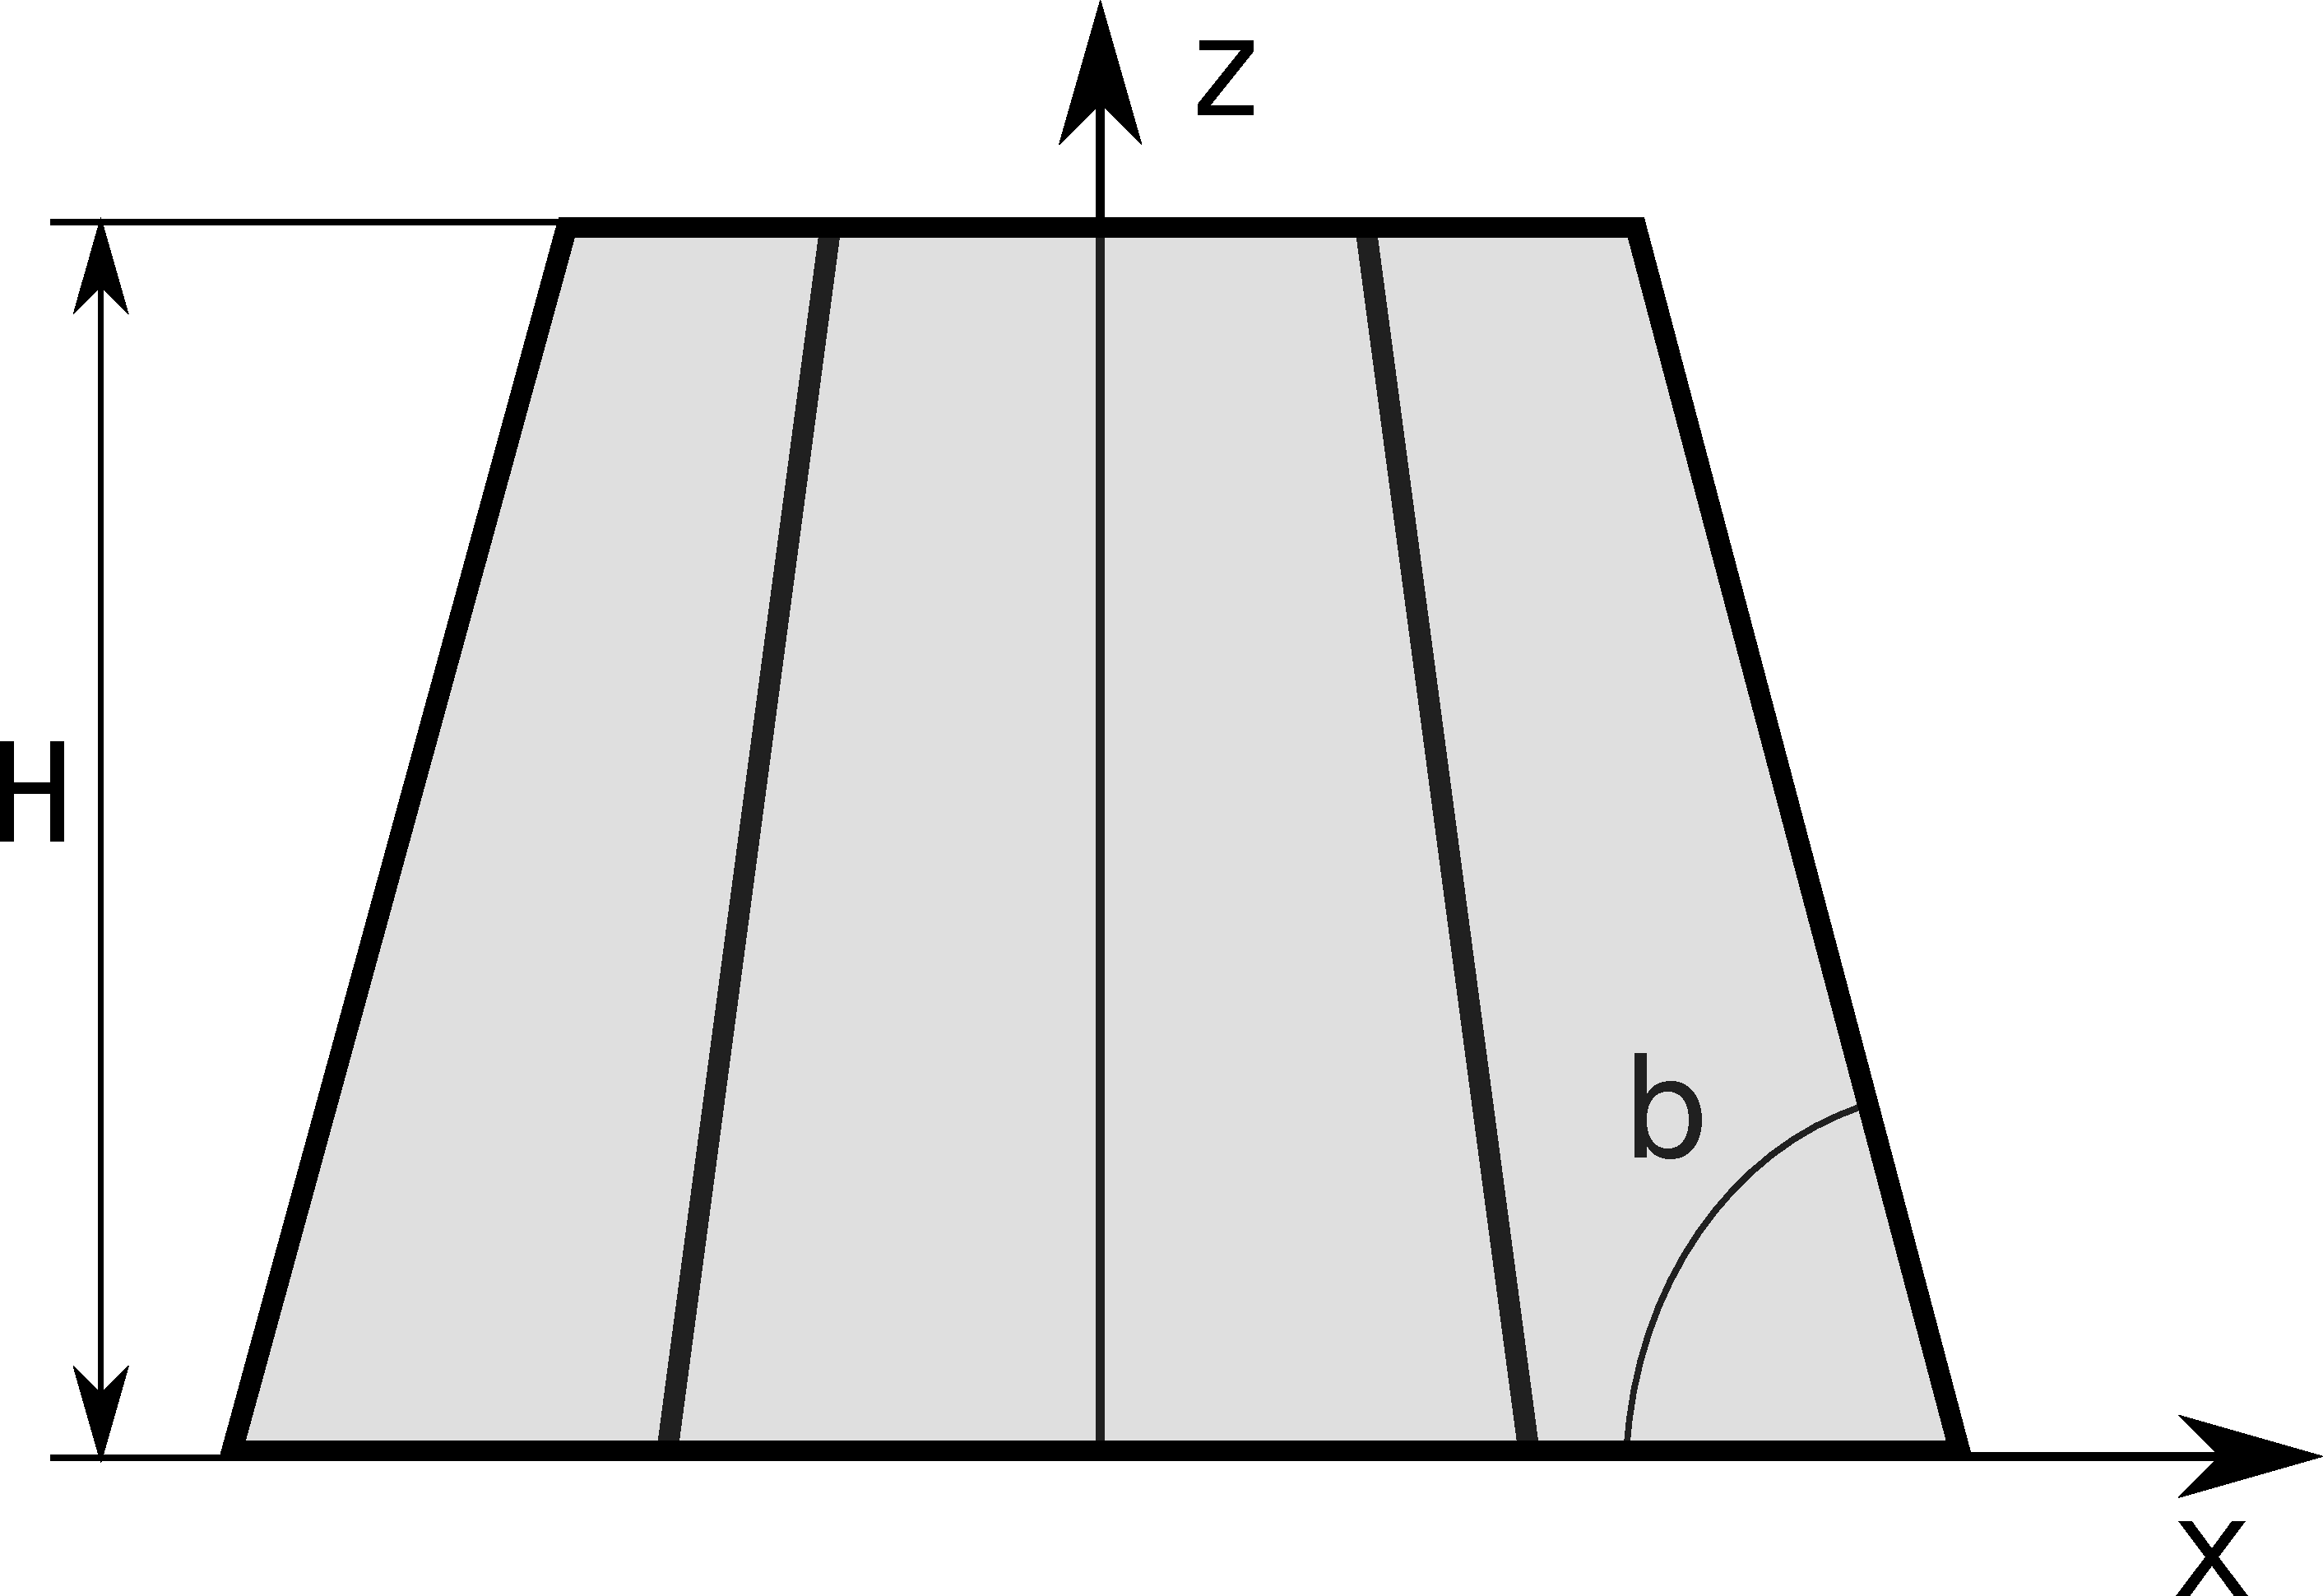
\includegraphics[width=.30\textwidth]{fig/cuts/Cone62dxz.pdf}}}
\hfill
\caption{A truncated hexagonal pyramid.}
\end{figure}

\FloatBarrier
\paragraph{Syntax and parameters}\strut\\[-2ex plus .2ex minus .2ex]
\begin{lstlisting}[language=python, style=eclipseboxed,numbers=none,nolol]
  FormFactorCone6(radius,height, alpha)
\end{lstlisting}
with the parameters
\begin{itemize}
\item \texttt{radius} of the regular hexagonal base, $R$,
\item \texttt{height}, $H$,
\item \texttt{alpha}, between the base and a side face, $\alpha$.
\end{itemize}
Note that the orthographic projection does not show~$\alpha$,
but the angle~$\beta$ between the base and a side edge.
They are related through $\sqrt{3}\tan \alpha = 2 \tan \beta$.
The following is written more conveniently in terms of~$\beta$.
The parameters must fulfill
\begin{displaymath}
  H \le (\tan\beta)R.
\end{displaymath}

\paragraph{Form factor etc}\strut\\
Notation:
\begin{equation*}
  R_H \coloneqq R-\frac{H}{\tan\beta},\quad
  \tilde{q}_x \coloneqq \frac{1}{2}q_y,\quad
  \tilde{q}_y \coloneqq \frac{\sqrt{3}}{2}q_y,\quad
  \tilde{q}_z \coloneqq (\tan\beta) q_z.
\end{equation*}
Results:
\begin{equation*}
  F = \frac{\sqrt{3}\, \e^{i\tilde q_z R}}{\tilde q_y ^2 - \tilde q_x^2}
    \int_{R_H}^R\!\d\rho\, \e^{-i\tilde q_z \rho}
\Big[\rho\tilde q_y \sinc(\tilde q_x\rho)\sin(\tilde q_y\rho)
+\cos(2\tilde q_x\rho)-\cos(\tilde q_y \rho)\cos(\tilde q_x\rho) \Big],
\end{equation*}
\begin{equation*}
  V = \tan\beta  \left( R^3- R_H^3 \right),
\end{equation*}
\begin{equation*}
  S =\dfrac{3\sqrt{3}R^2}{2}.
\end{equation*}

\paragraph{Example}\strut\\
Figure~\ref{fig:FFCone6Ex} shows the normalized intensity
$|F|^2/V^2$, computed with $R=10$~nm, $H=13$~nm, and
$\alpha=60^{\circ}$.

\begin{figure}[H]
\begin{center}
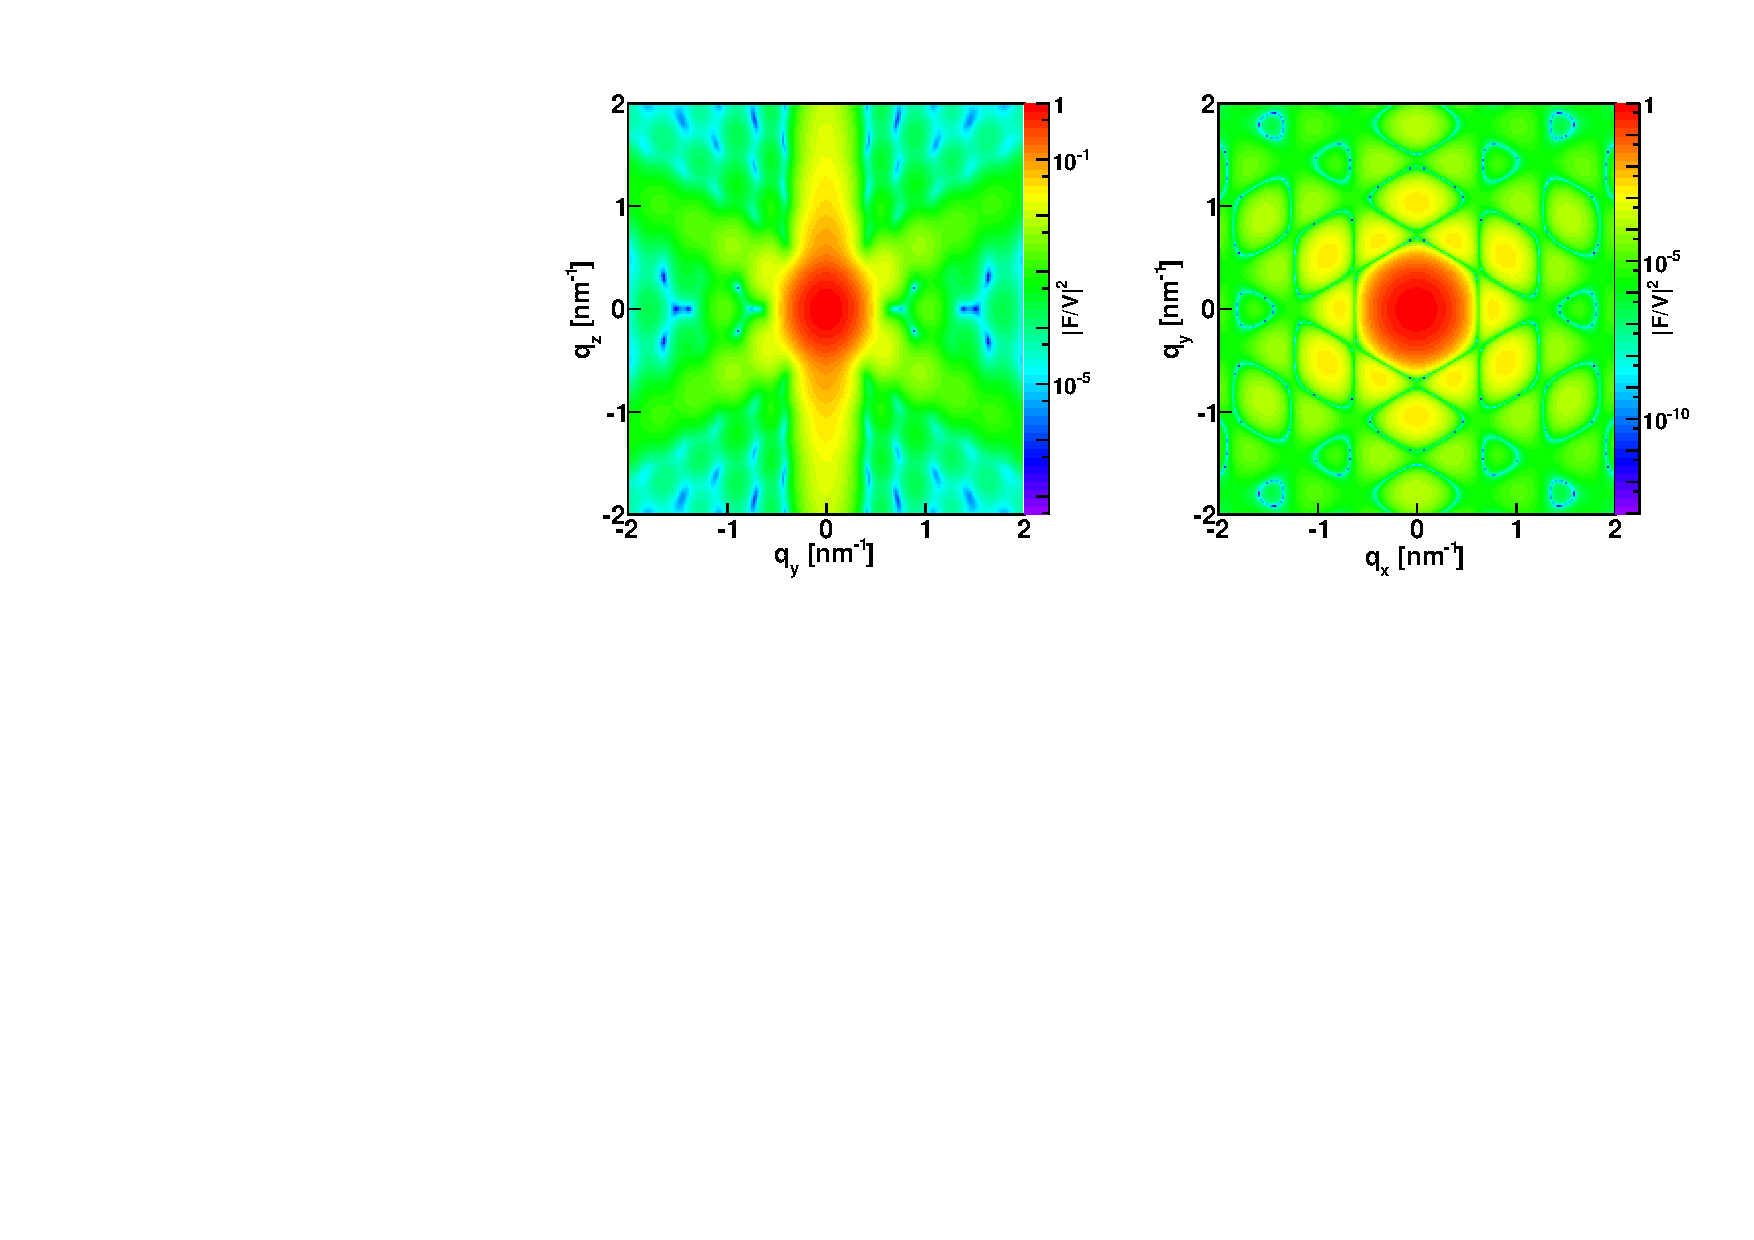
\includegraphics[angle=-90,width=\textwidth]{fig/ff/figffcone6.pdf}
\end{center}
\caption{Normalized intensity for the form factor of a Cone6 plotted against ($q_y$, $q_z$) and ($q_x$, $q_y$) and computed with \Code{FormFactorCone6(10.*nanometer, 13.*nanometer, 60.*degree)}.}
\label{fig:FFCone6Ex}
\end{figure}

\paragraph{References}\strut\\
Hopefully agrees with \E{Cone6} form factor of \IsGISAXS\
\cite[Eq.~2.32]{Laz08} \cite[Eq.~222]{ReLL09},
except for different parametrization.

%-------------------------------------------------------------------------------
\clearpage
\subsection{Cuboctahedron} \label{sec:Cuboctahedron}
  \index{Cuboctahedron (form factor)}
  \index{FormFactorCuboctahedron@\Code{FormFactorCuboctahedron}}
%-------------------------------------------------------------------------------

\paragraph{Real-space geometry}\strut\\

\begin{figure}[H]
\hfill
\subfigure[Perspective]{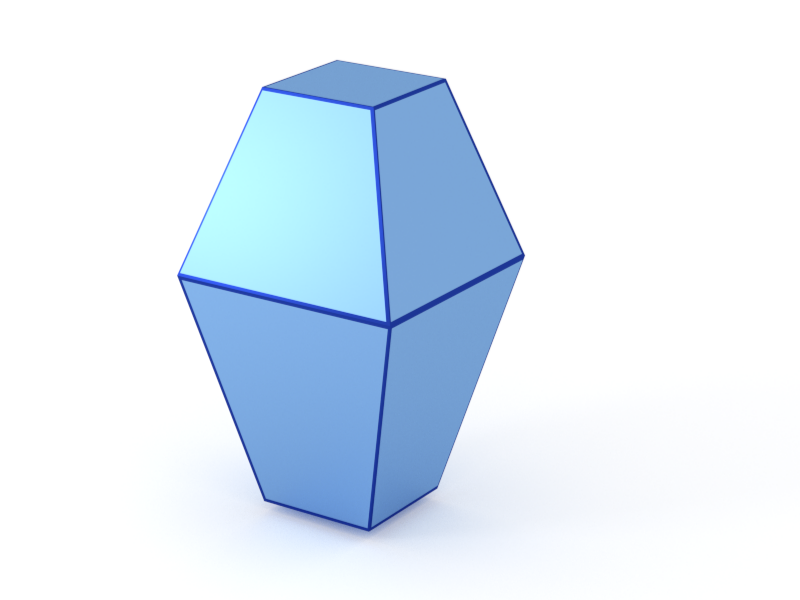
\includegraphics[width=.24\textwidth]{fig/blue/Cuboctahedron3d.png}}
\hfill
\subfigure[Top view]{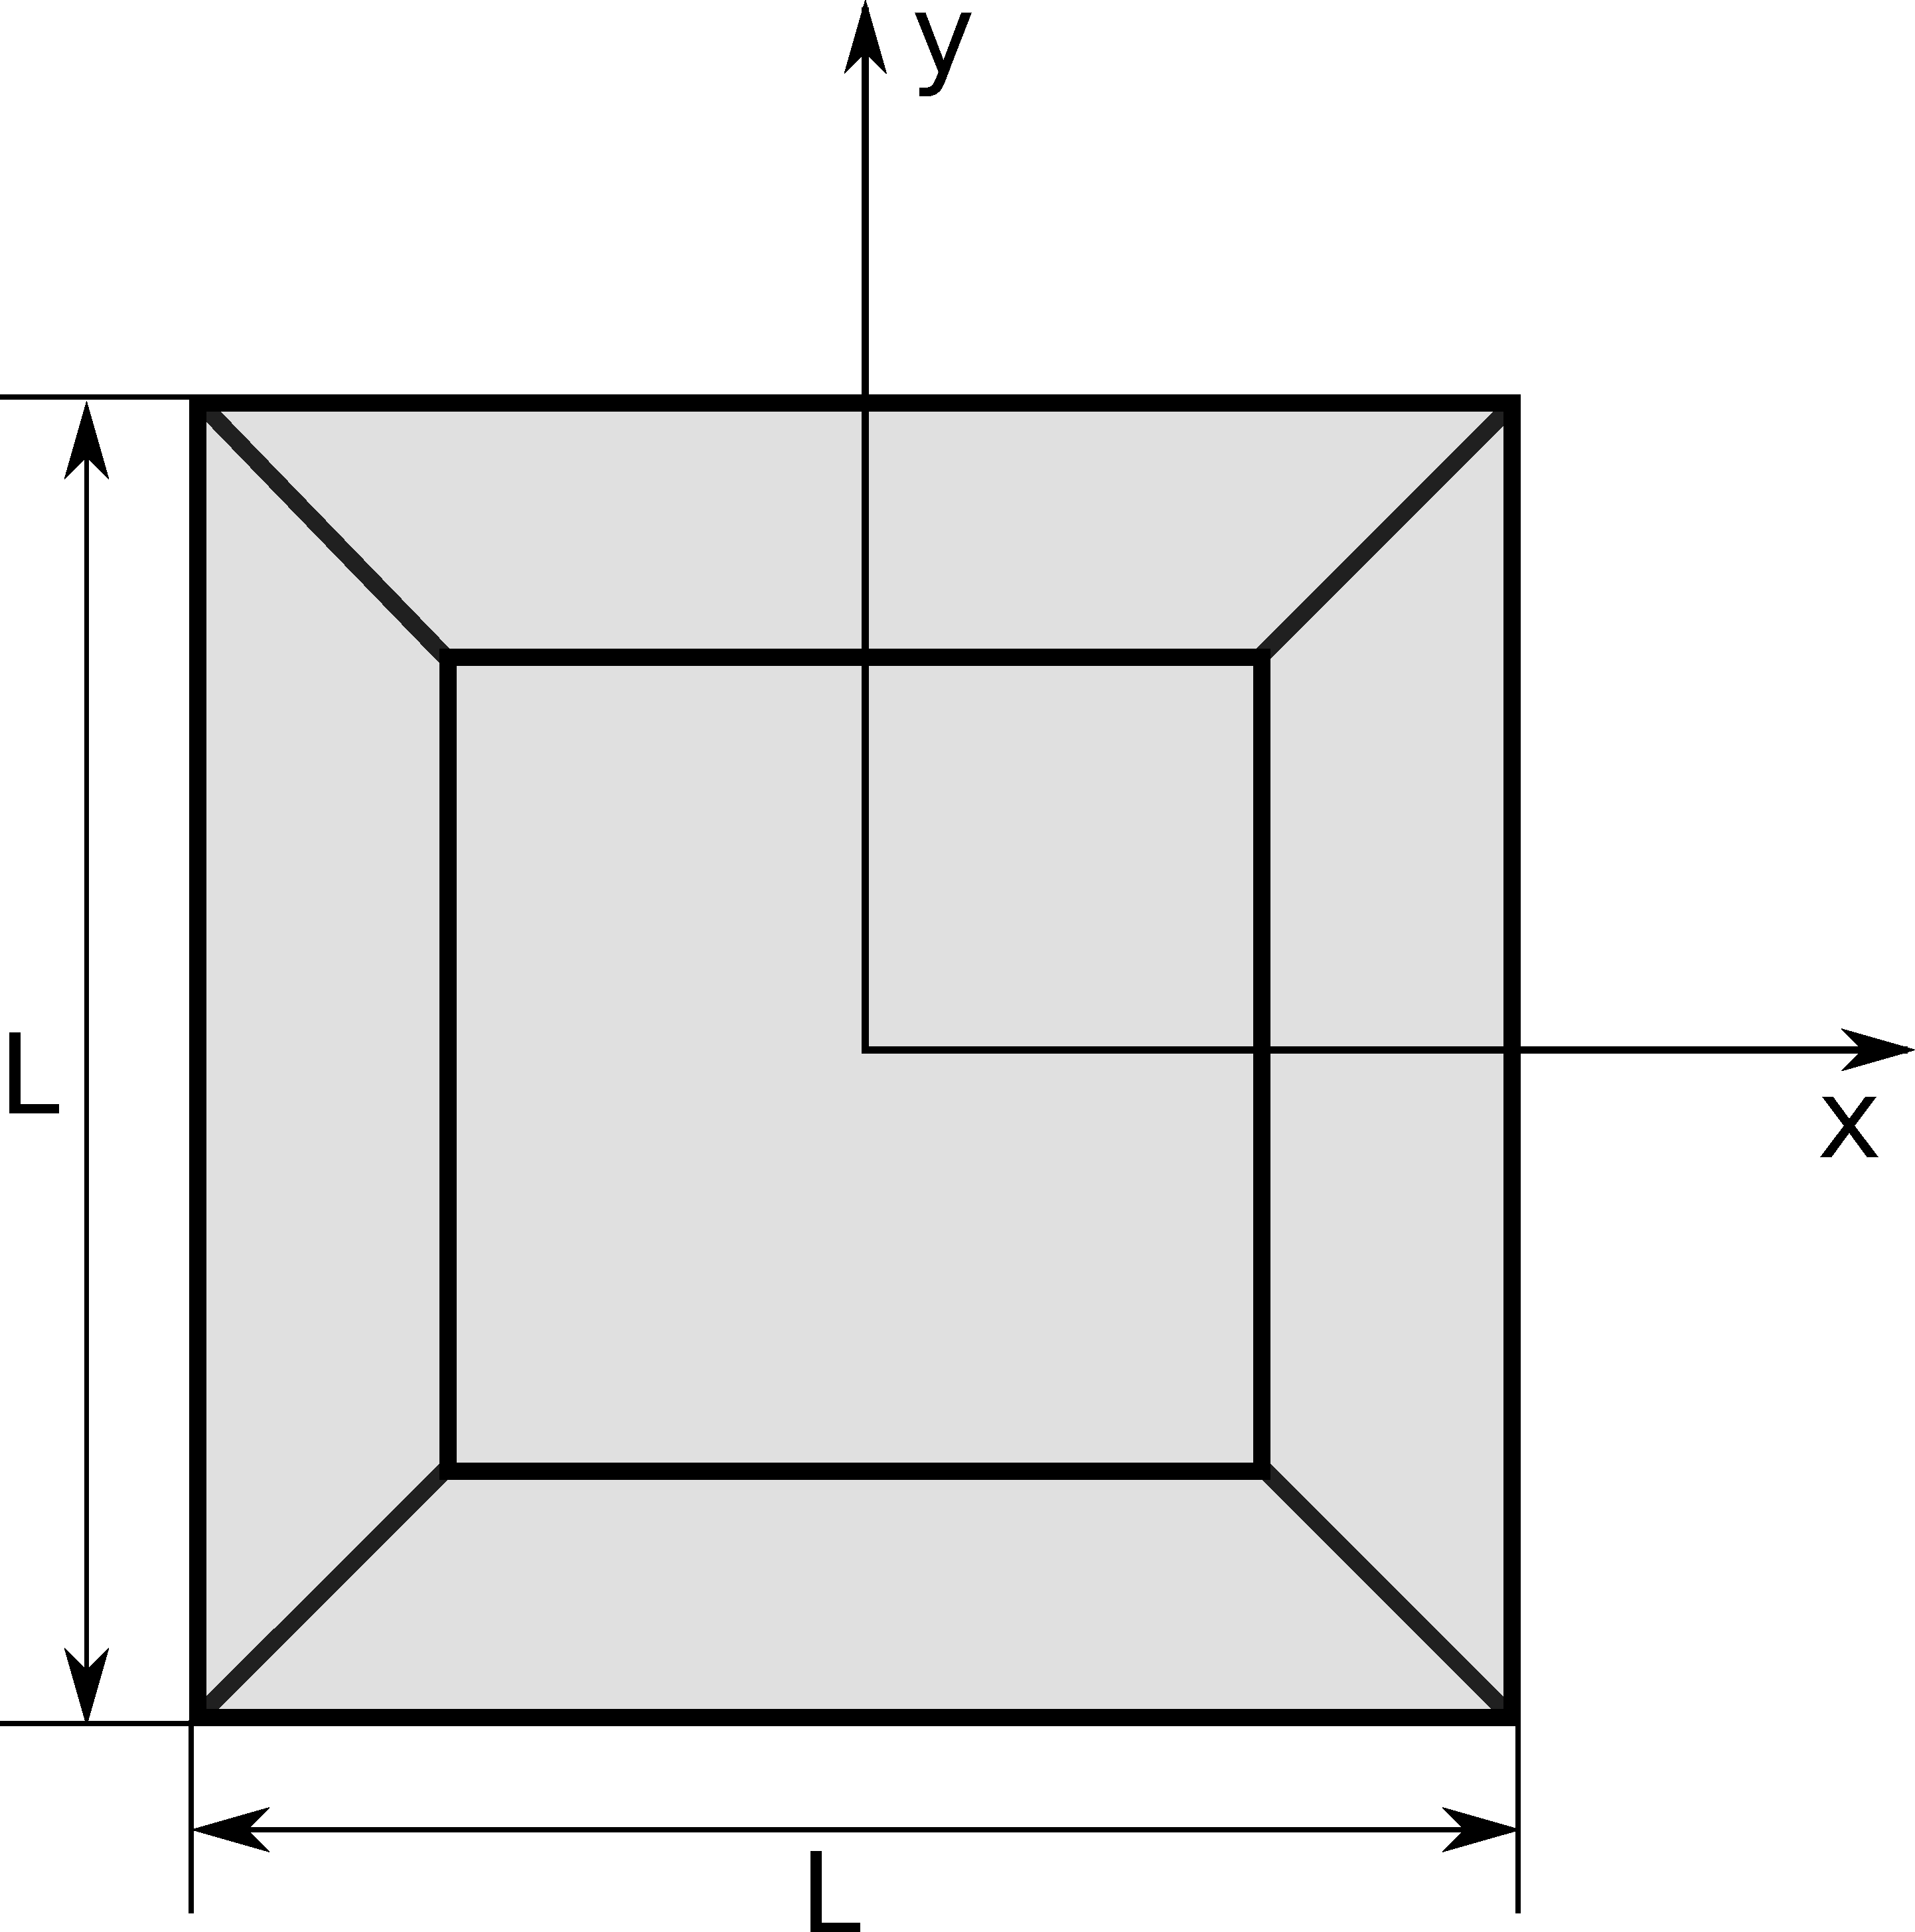
\includegraphics[width=.30\textwidth]{fig/cuts/Cuboctahedron2dxy.pdf}}
\hfill
\subfigure[Side view]{\raisebox{2mm}{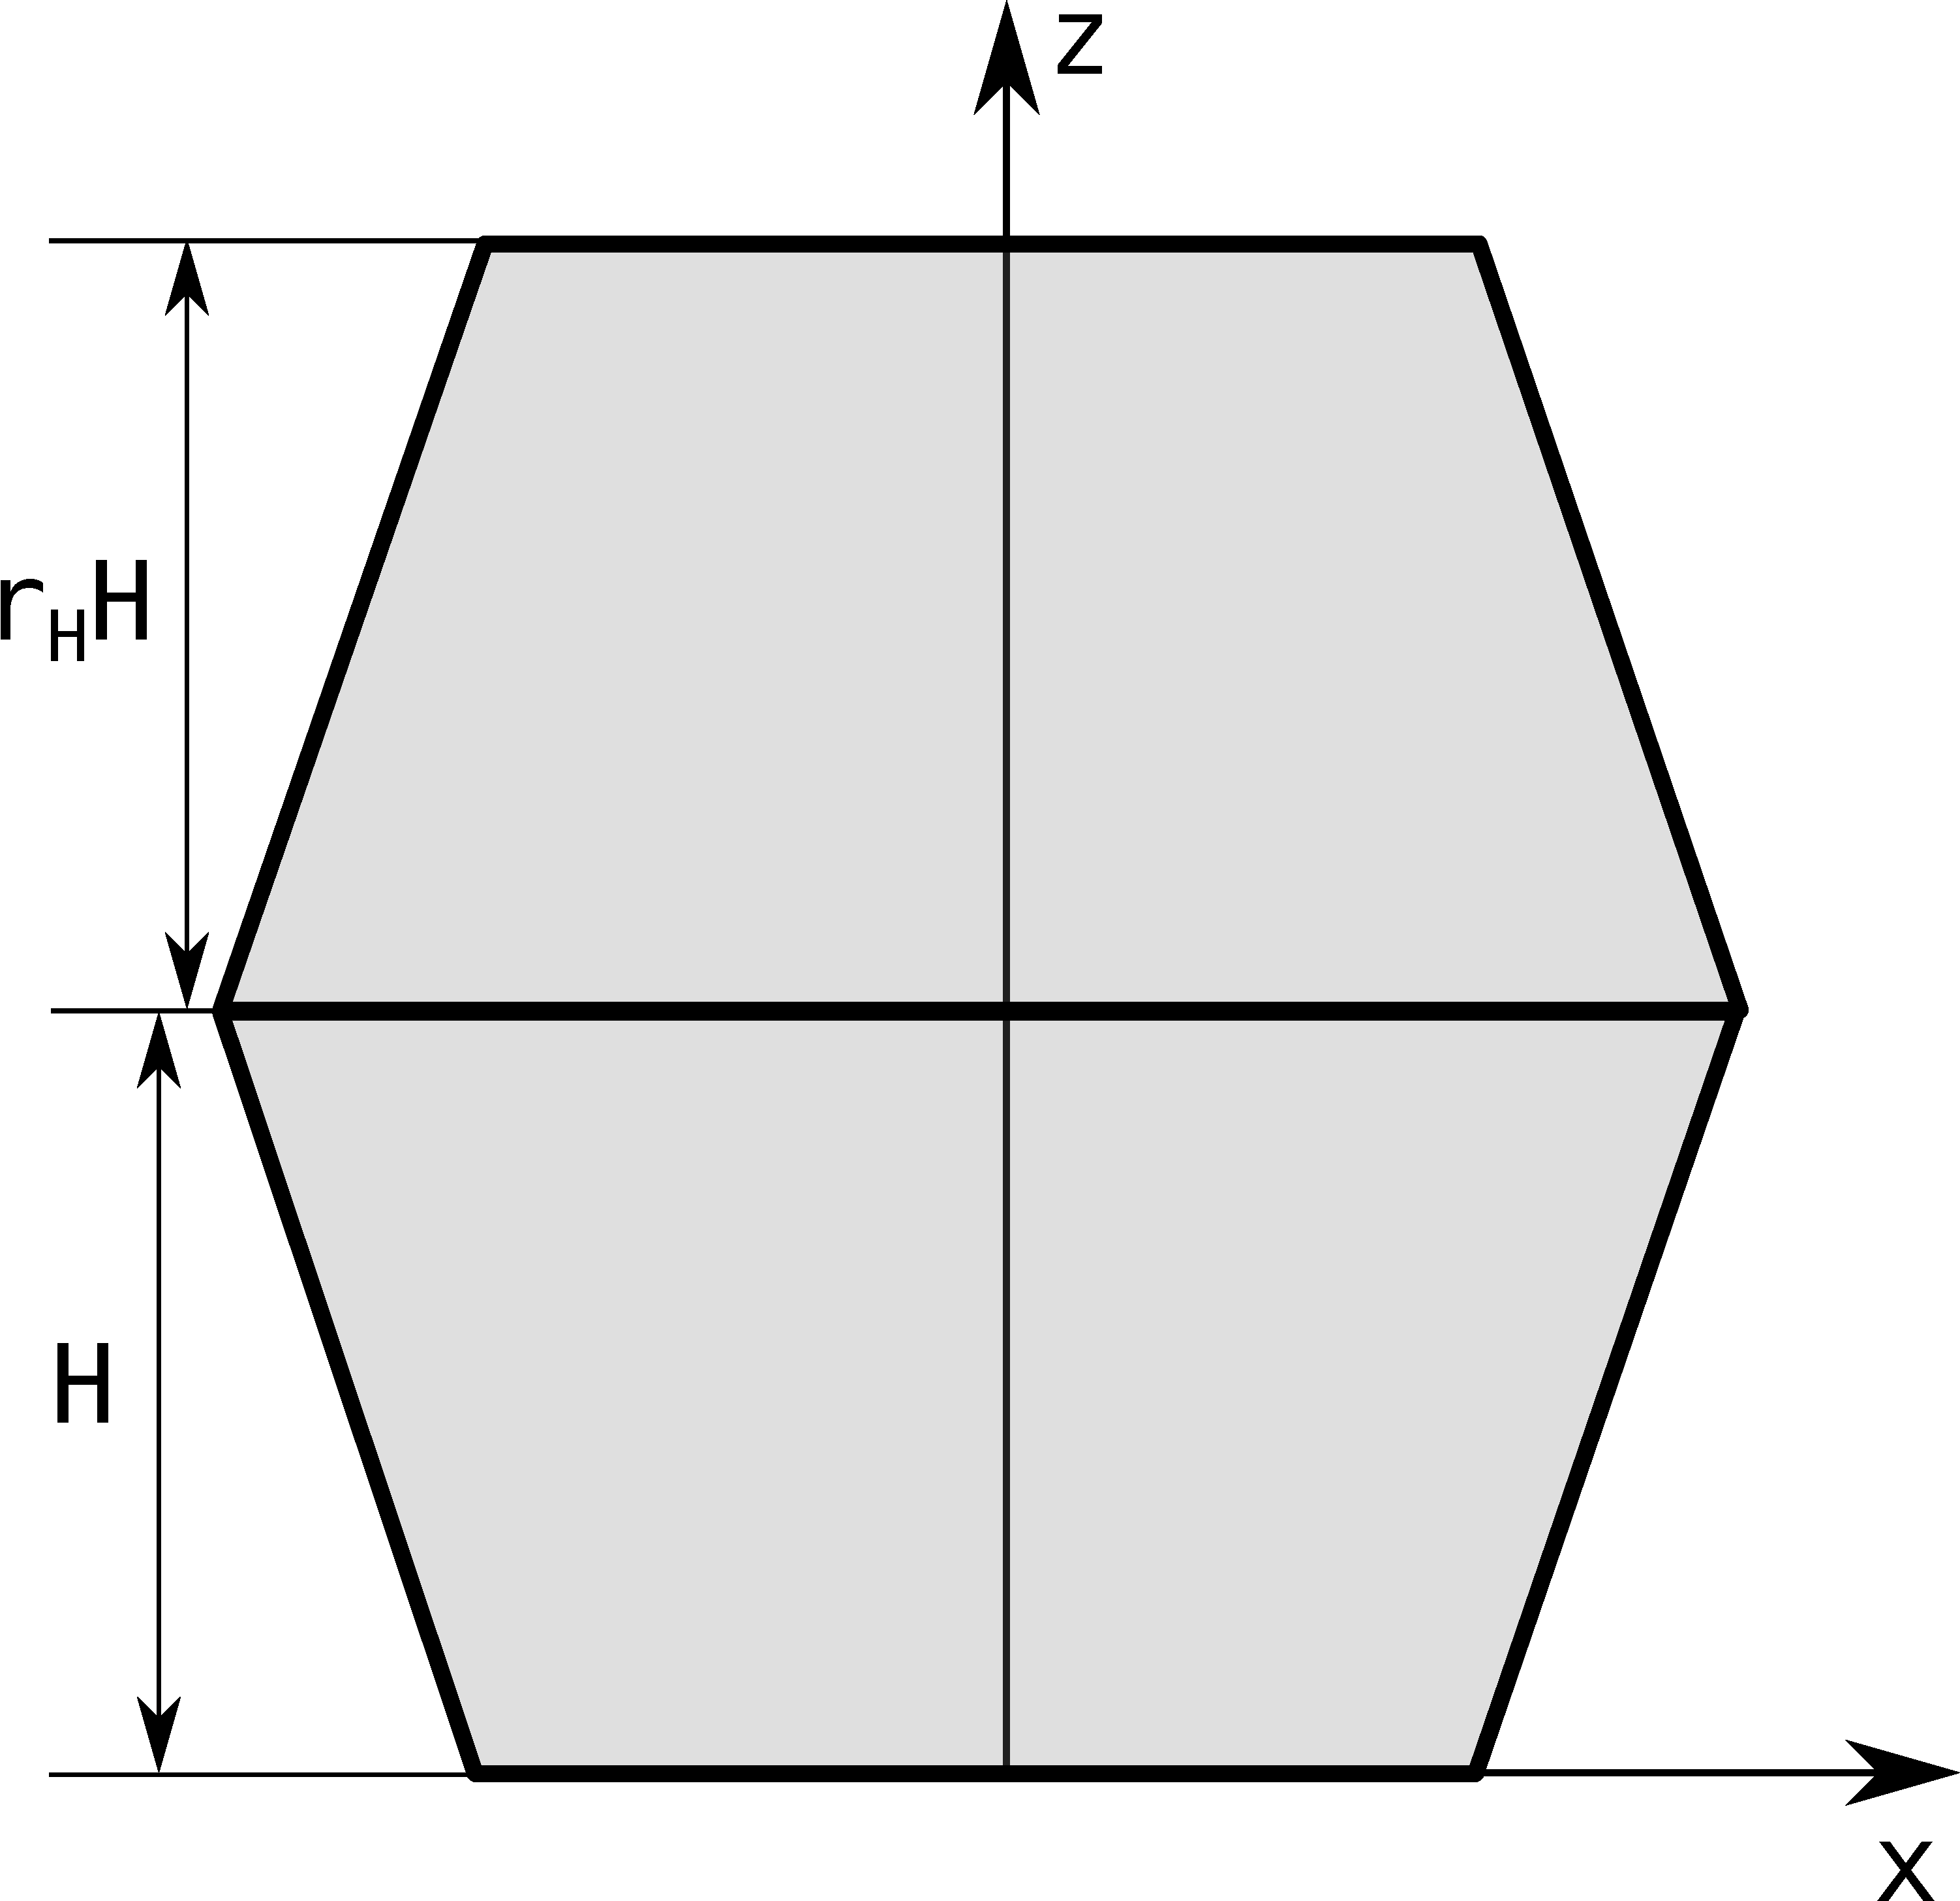
\includegraphics[width=.30\textwidth]{fig/cuts/Cuboctahedron2dxz.pdf}}}
\hfill
\caption{A compound of two truncated pyramids with a common square base
and opposite orientations.}
\end{figure}

\FloatBarrier

\paragraph{Syntax and parameters}\strut\\[-2ex plus .2ex minus .2ex]
\begin{lstlisting}[language=python, style=eclipseboxed,numbers=none,nolol]
  FormFactorCuboctahedron(length, height, height_ratio, alpha)
\end{lstlisting}
with the parameters
\begin{itemize}
\item \texttt{length} of the shared square base, $L$,
\item \texttt{height} of the bottom pyramid, $H$,
\item \texttt{height\_ratio} between the top and the bottom pyramid, $r_H$,
\item \texttt{alpha}, angle between the base and a side face, $\alpha$.
\end{itemize}
They must fulfill
\begin{displaymath}
  H \le \frac{\tan\alpha}{2} L
  \quad\text{and}\quad
  r_h H \le \frac{\tan\alpha}{2} L.
\end{displaymath}


\paragraph{Form factor etc}\strut\\
Using the form factor of a square pyramid $F_\text{Py}$
(Sect.~\ref{sec:Pyramid}):
\begin{equation*}
F=\exp(iq_zH)\Big[F_\text{Py}(q_x,q_y, q_z, L, r_H H,\alpha)
                 +F_\text{Py}(q_x, q_y, -q_z, L, H, \alpha))\Big],
\end{equation*}
\begin{equation*}
  V= \dfrac{1}{6} \tan(\alpha)L^3 \Big[ 2
         - \Big(1 - \dfrac{2H }{L\tan(\alpha)} \Big)^3
           - \Big(1 - \dfrac{2 r_H
             H}{L\tan(\alpha) }\Big)^3\Big],
\end{equation*}
\begin{equation*}
  S =L^2.
\end{equation*}

\paragraph{Example}\strut\\
Figure~\ref{fig:FFcuboctahEx} shows the normalized intensity $|F|^2/V^2$, computed with $L=20$~nm, $H=13$~nm, $r_H=0.7$, and $\alpha=60^{\circ}$.
\begin{figure}[H]
\begin{center}
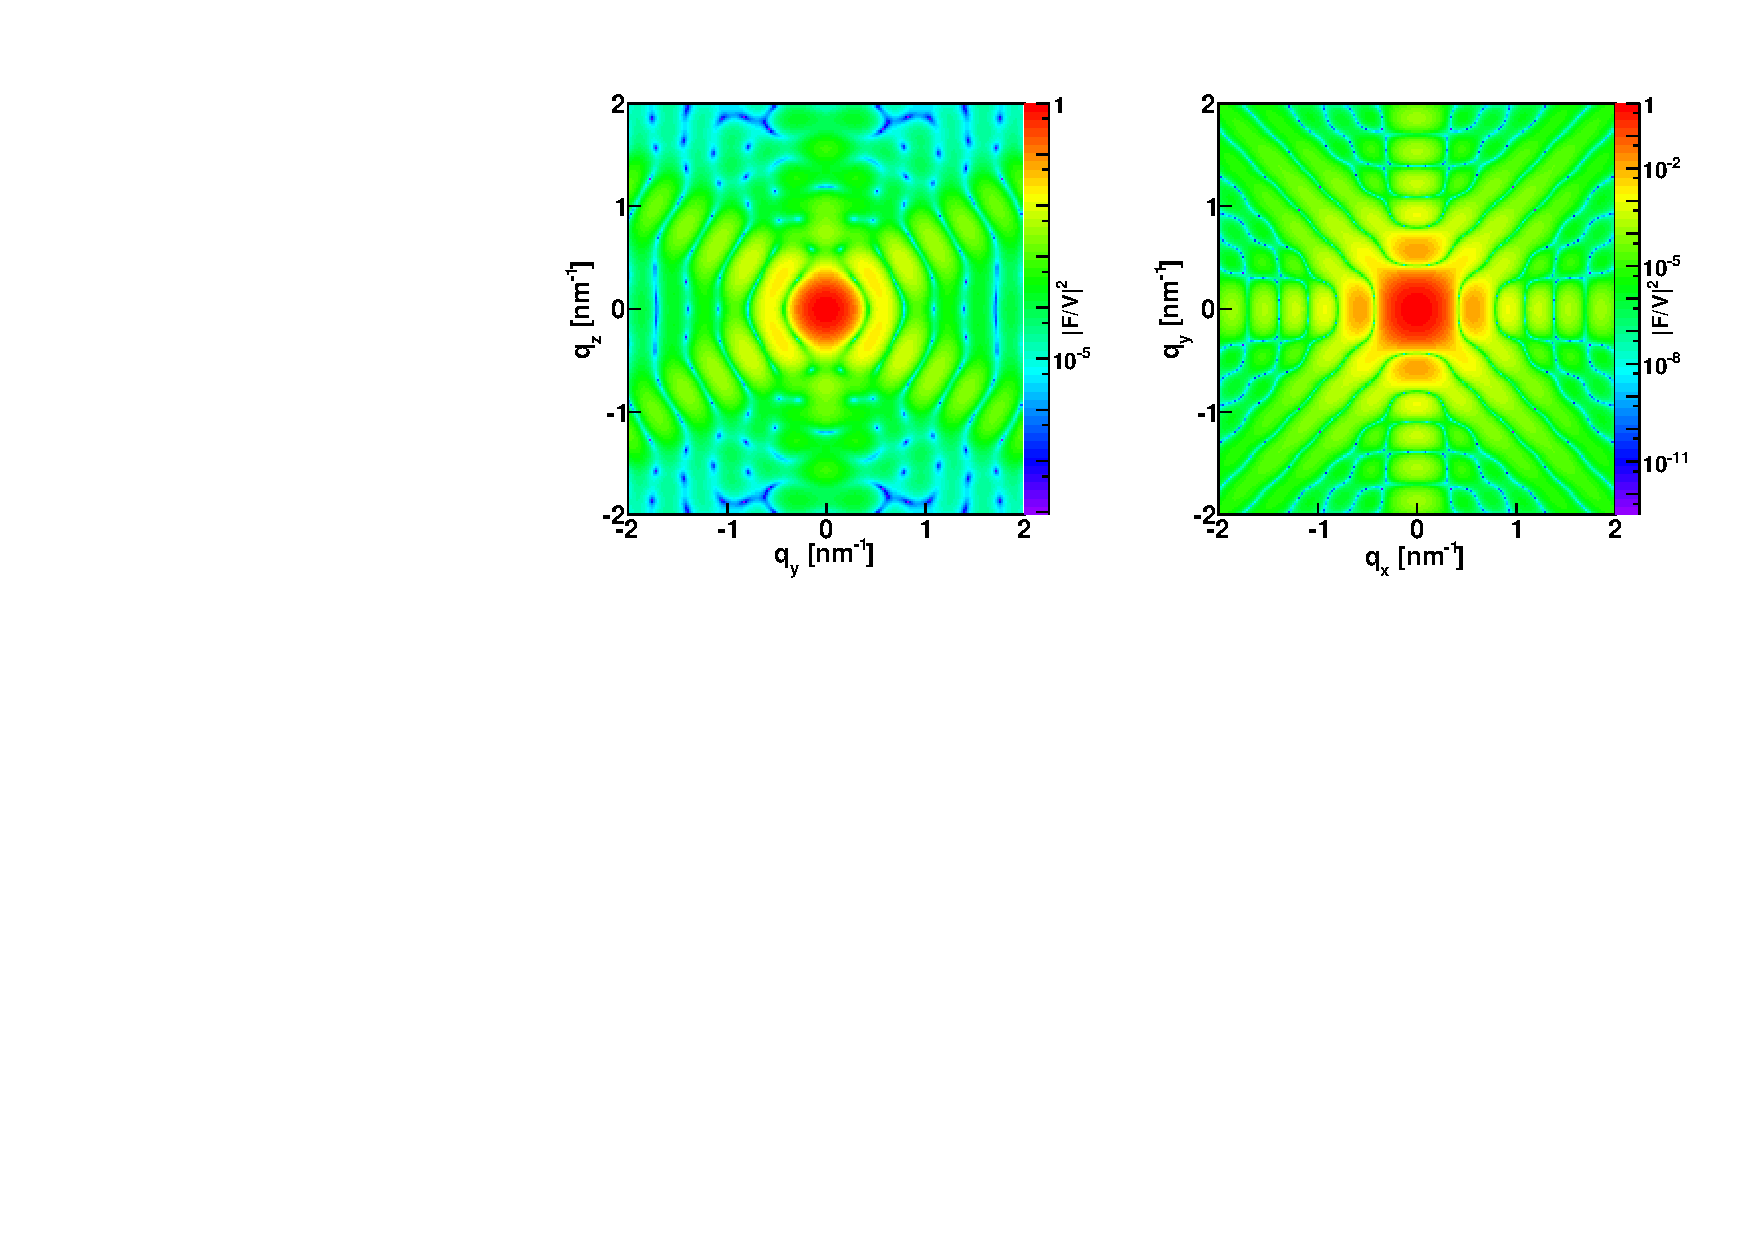
\includegraphics[angle=-90,width=\textwidth]{fig/ff/figffcuboctah.pdf}
\end{center}
\caption{Normalized intensity for the form factor of a cuboctahedron plotted against ($q_y$, $q_z$) and  ($q_x$, $q_y$) and computed with \Code{FormFactorCuboctahedron(20.*nanometer, 13.*nanometer, 0.7, 60.*degree)}.}
\label{fig:FFcuboctahEx}
\end{figure}

\paragraph{References}\strut\\
Agrees with \E{Cuboctahedron} form factor of \IsGISAXS\
\cite[Eq.~2.34]{Laz08} \cite[Eq.~218]{ReLL09},
except for different parametrization $L=2R_{\rm{\Code{IsGISAXS}}}$.

%-------------------------------------------------------------------------------
\clearpage
\subsection{Cylinder} \label{sec:Cylinder}
  \index{Cylinder (form factor)}
  \index{FormFactorCylinder@\Code{FormFactorCylinder}}
%-------------------------------------------------------------------------------
 
\paragraph{Real-space geometry}\strut\\

\begin{figure}[H]
\hfill
\subfigure[Perspective]{
\includegraphics[width=.24\textwidth]{fig/blue/Cylinder3d.png}}
\hfill
\subfigure[Top view]{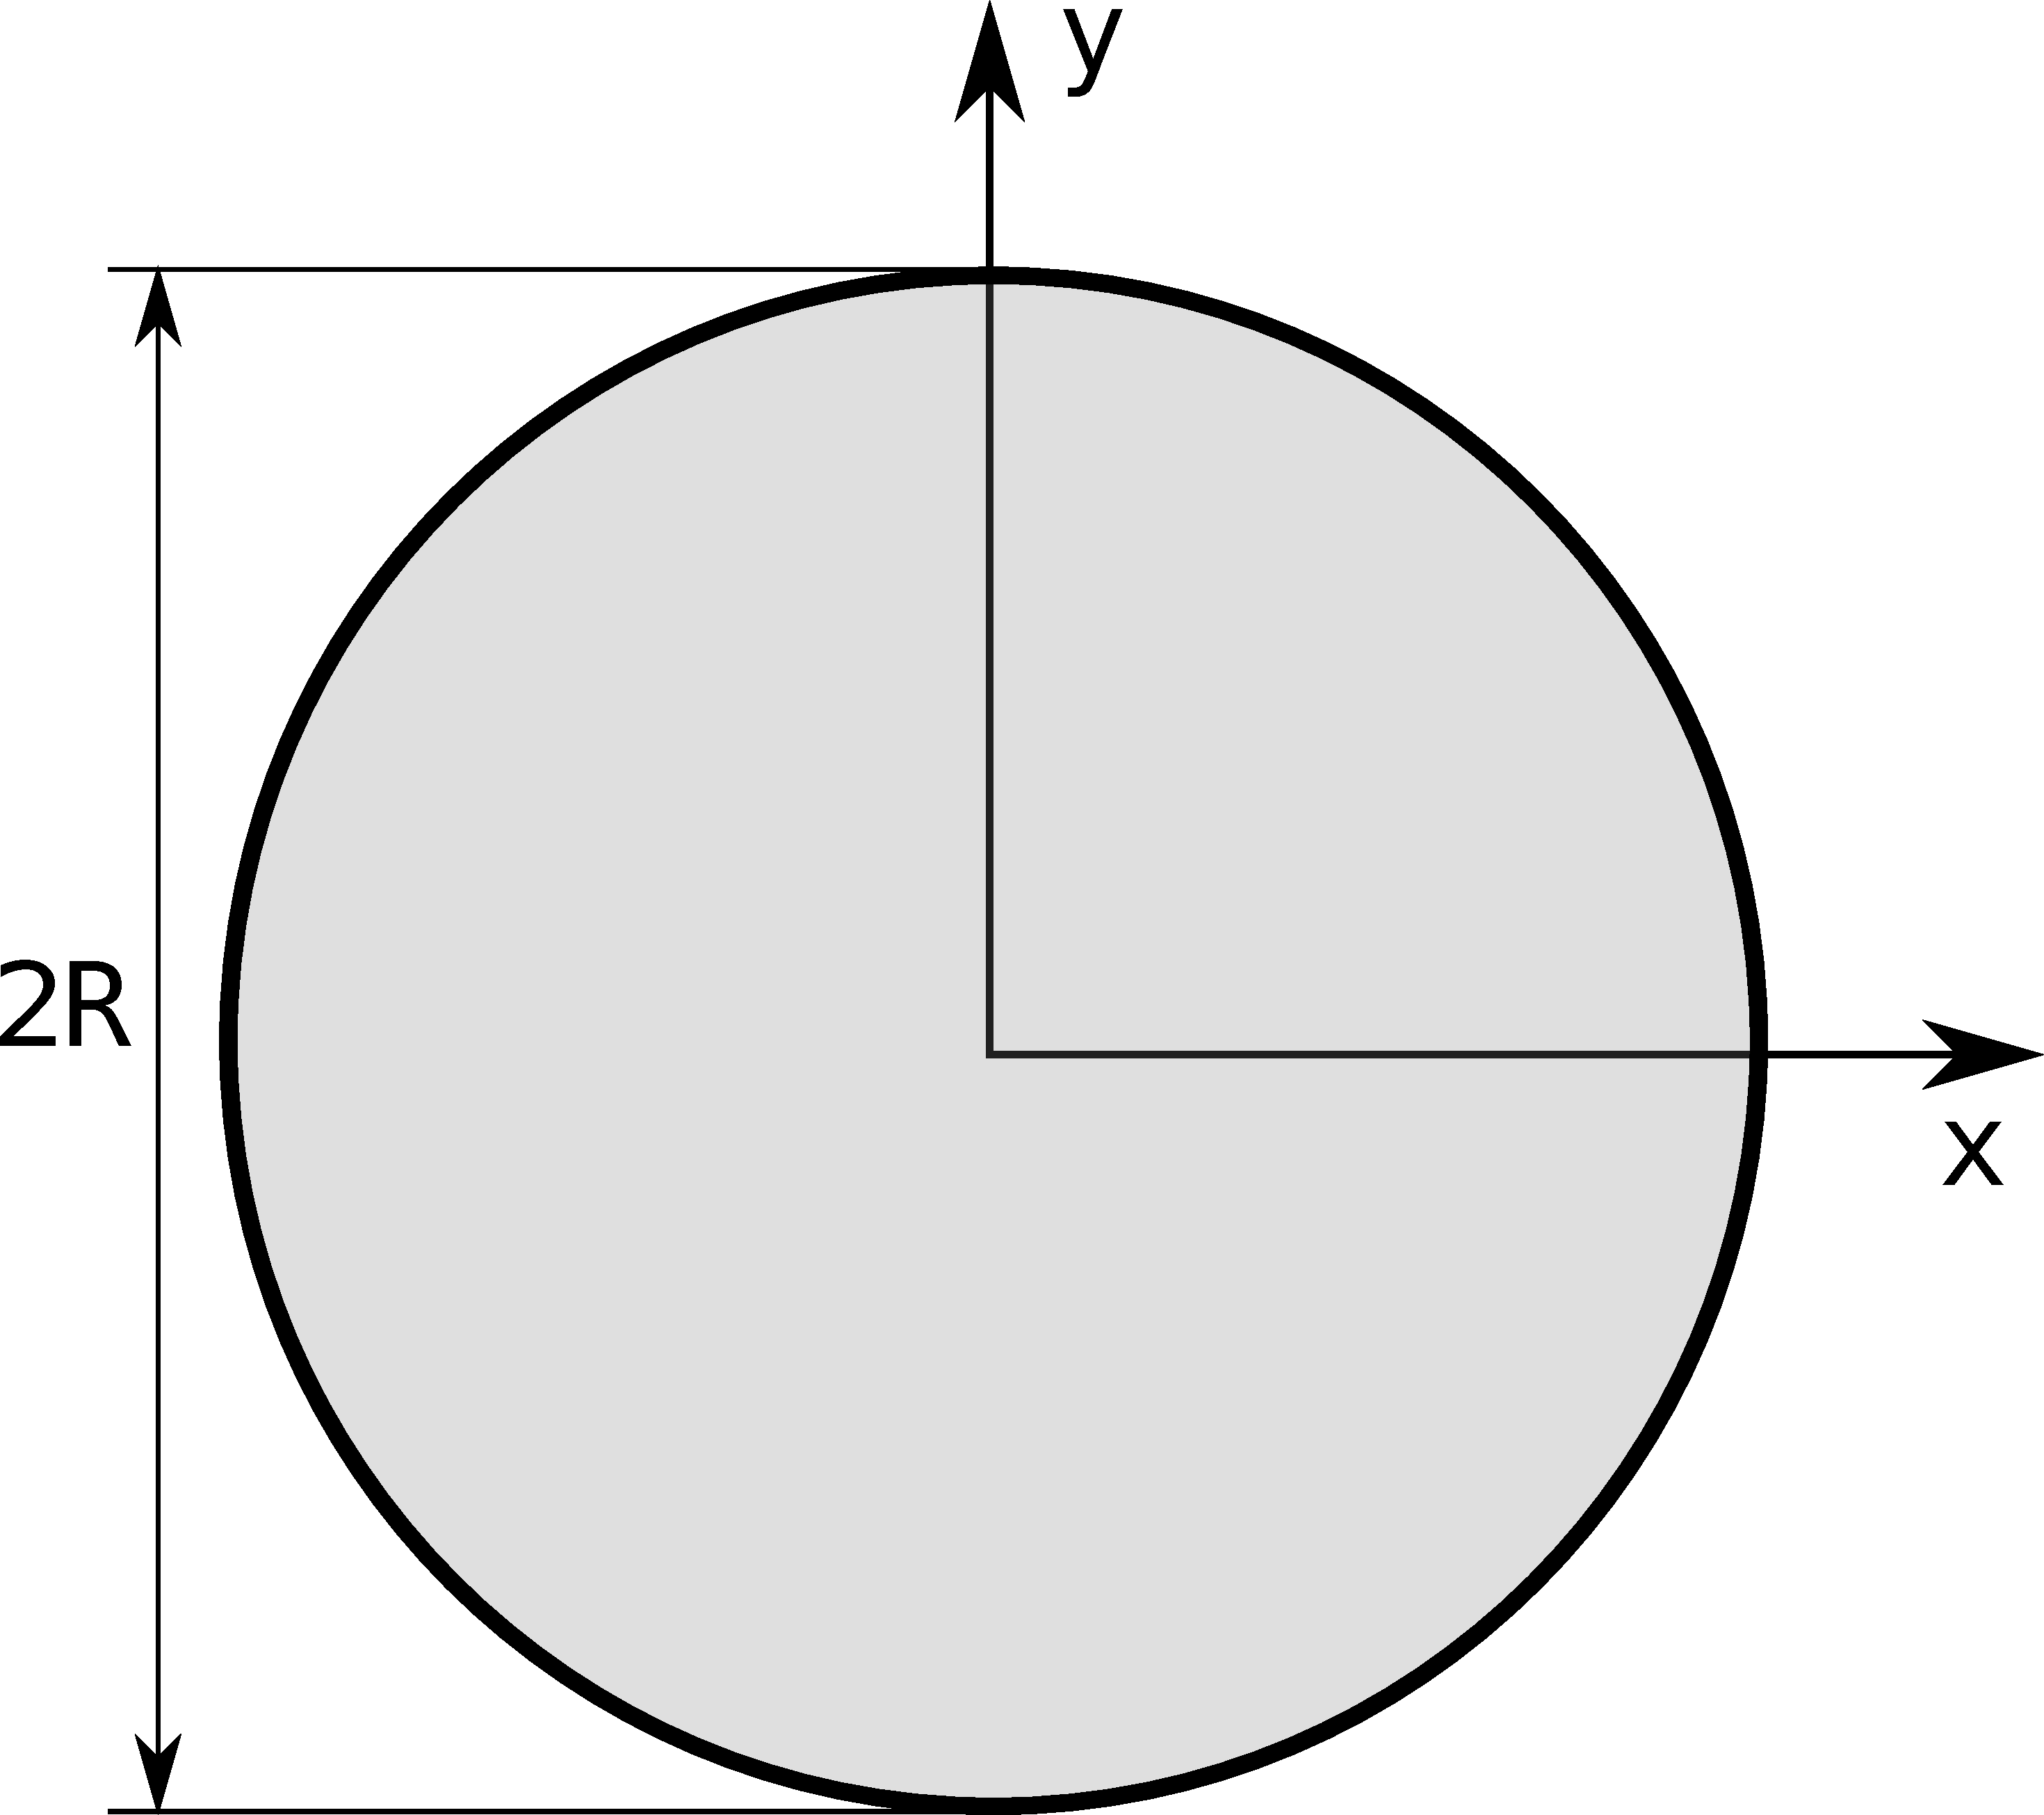
\includegraphics[width=.30\textwidth]{fig/cuts/Cylinder2dxy.pdf}}
\hfill
\subfigure[Side view]{\raisebox{-2.5mm}{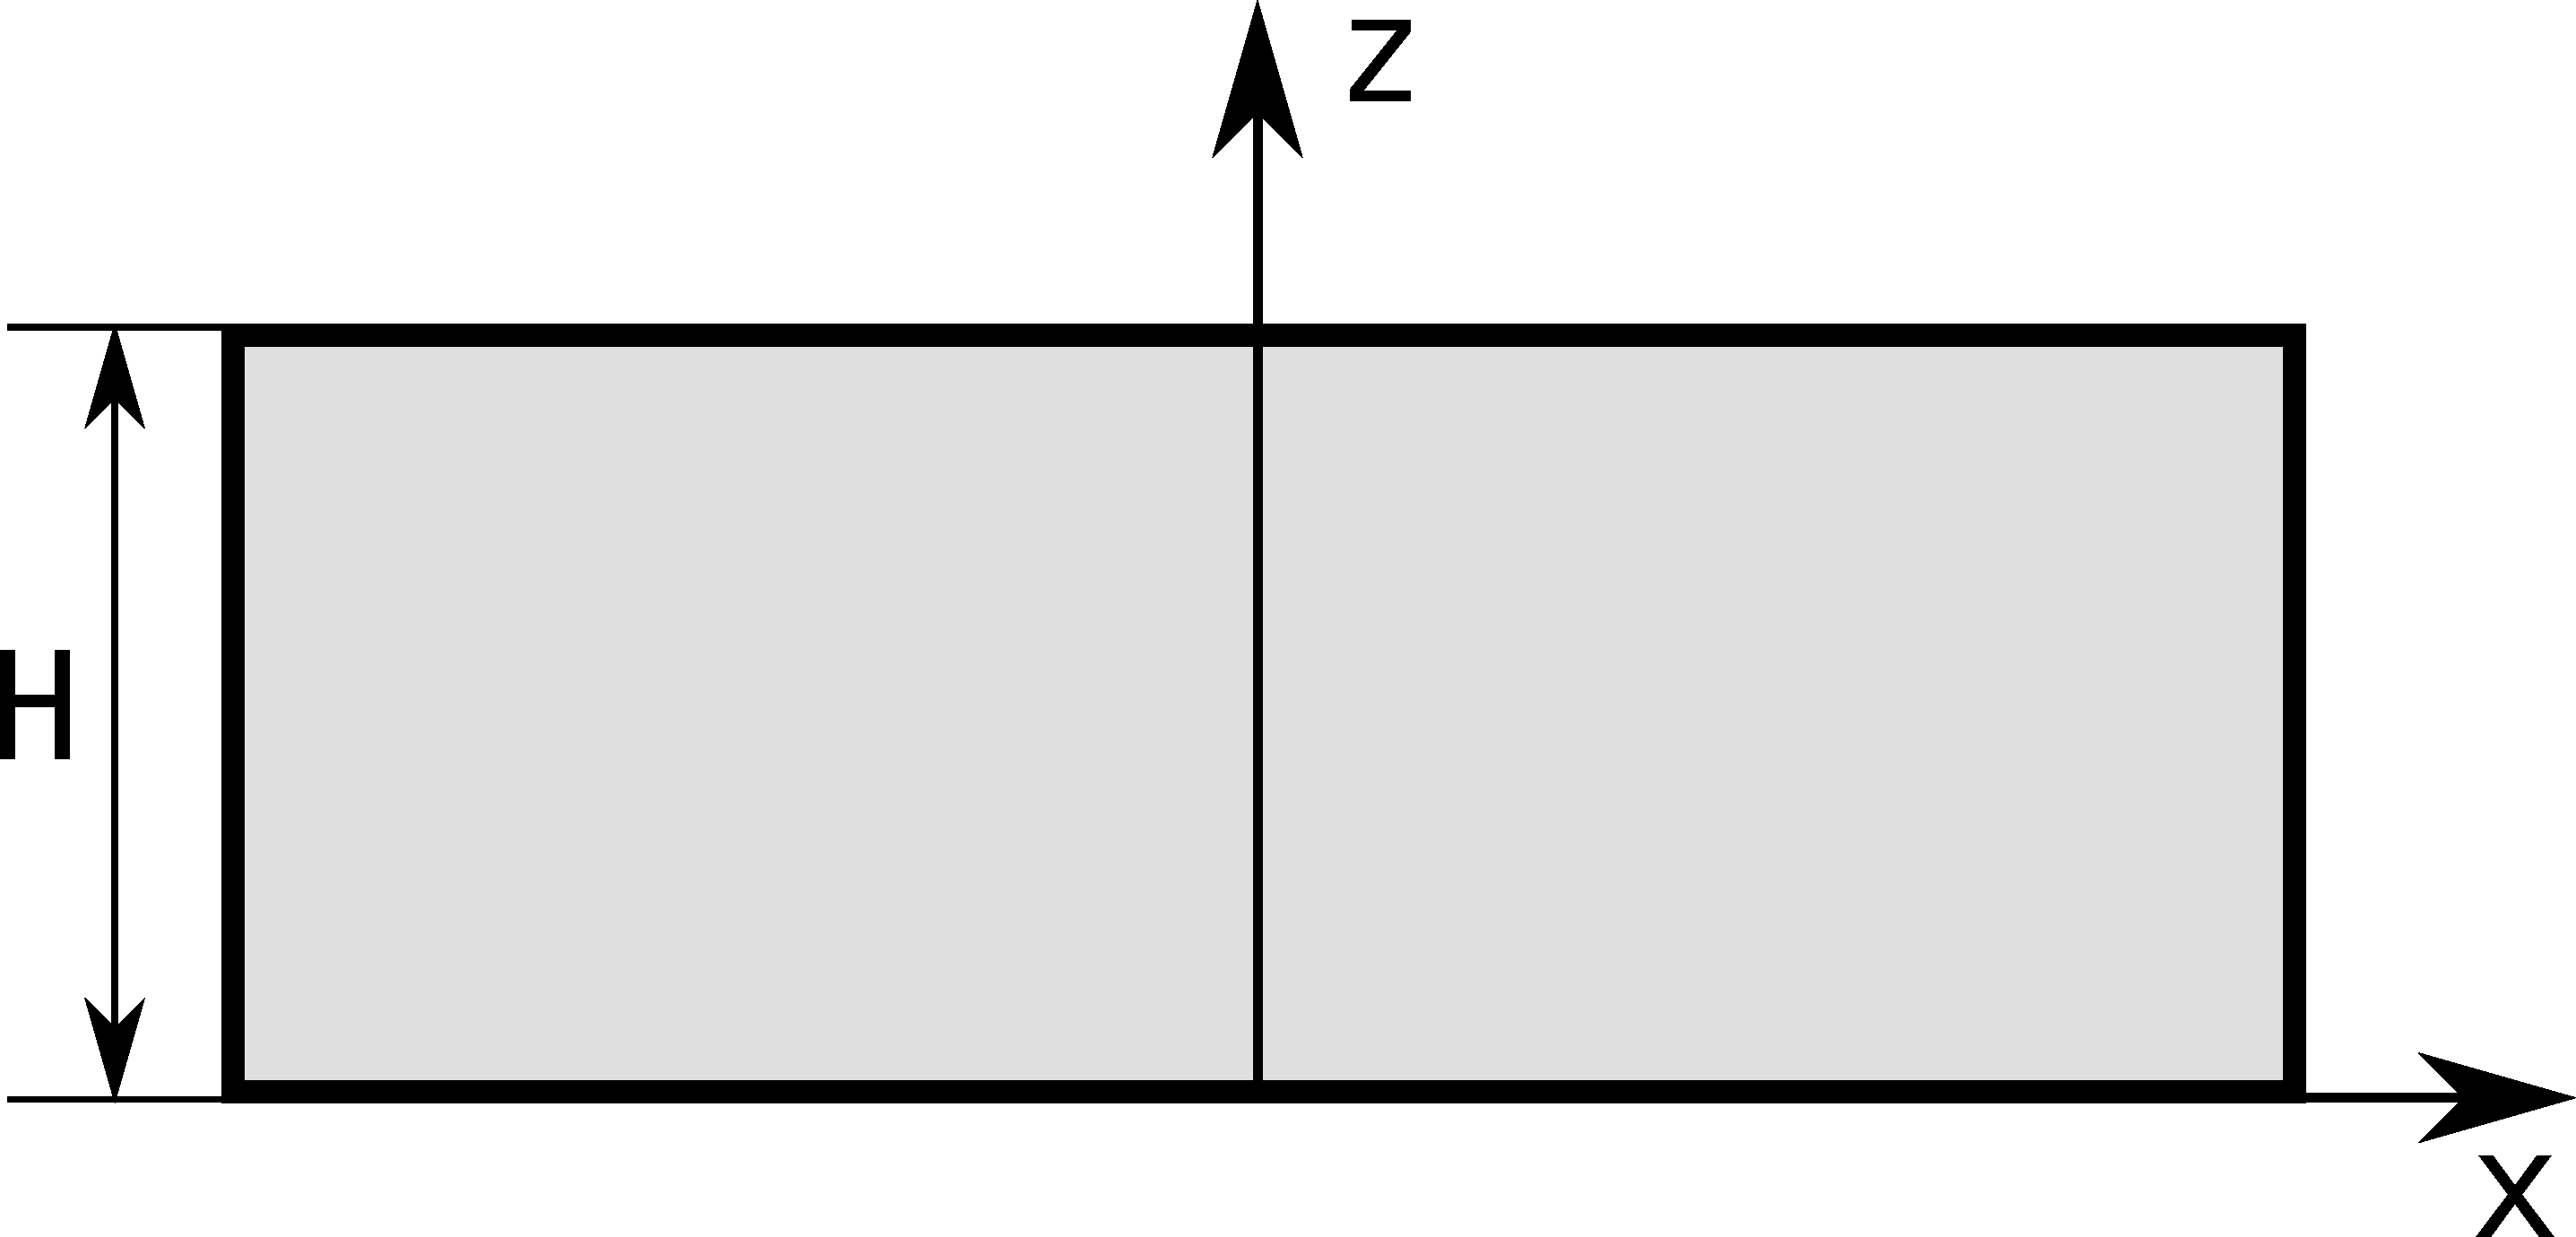
\includegraphics[width=.30\textwidth]{fig/cuts/Cylinder2dxz.pdf}}}
\hfill
\caption{An upright circular cylinder.}
\end{figure}

\paragraph{Syntax and parameters}\strut\\[-2ex plus .2ex minus .2ex]
\begin{lstlisting}[language=python, style=eclipseboxed,numbers=none,nolol]
  FormFactorCylinder(radius, height)
\end{lstlisting}
with the parameters
\begin{itemize}
\item \texttt{radius} of the circular base, $R$, 
\item \texttt{height}, $H$.
\end{itemize}


\paragraph{Form factor etc}\strut\\
Notation:
\begin{equation*}
  q_{\parallel} \coloneqq \sqrt{q_x^2+q_y^2}.
\end{equation*}
Results:
\begin{equation*}
  F=  2\pi R^2 H  \sinc\left(q_ z \frac{H}{2}\right) \exp\left(i q_ z \frac{H}{2}\right) 
    \frac{J_1(q_{\parallel} R )}{q_{\parallel} R },
\end{equation*}
\begin{equation*}
  V = \pi R^2 H,
\end{equation*}
\begin{equation*}
  S=\pi R^2.
\end{equation*}

\paragraph{Example}\strut\\
Figure~\ref{fig:FFcylinderEx} shows the normalized intensity
$|F|^2/V^2$, computed with $R=8$~nm and \mbox{$H=16$~nm.}
\begin{figure}[H]
\begin{center}
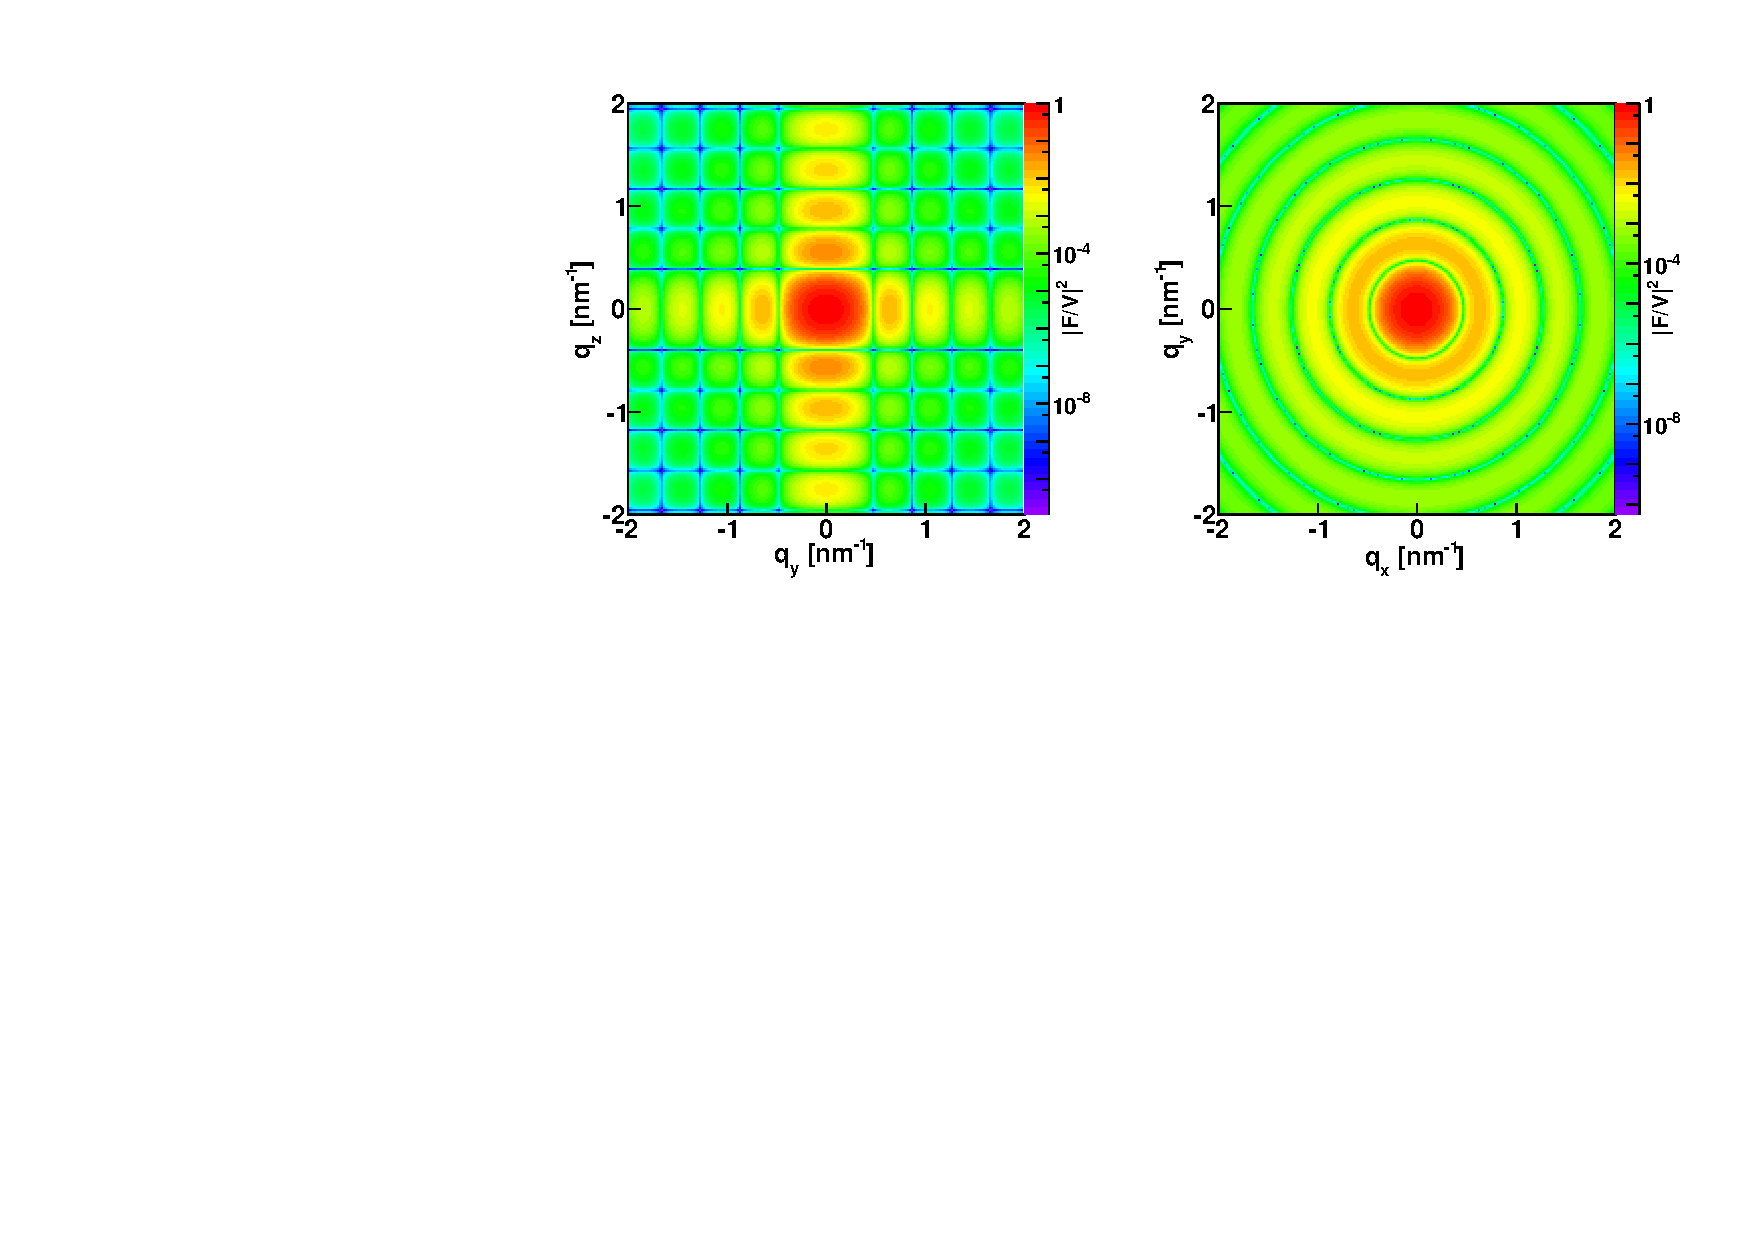
\includegraphics[angle=-90,width=\textwidth]{fig/ff/figffcylinder.pdf}
\end{center}
\caption{Normalized intensity for the form factor of a cylinder plotted against ($q_y$, $q_z$) and  ($q_x$, $q_y$.) It
has been  computed with \Code{FormFactorCylinder(8.*nanometer, 16.*nanometer)}.}
\label{fig:FFcylinderEx}
\end{figure}

\paragraph{References}\strut\\
Agrees with \E{Cylinder} form factor of \IsGISAXS\
\cite[Eq.~2.27]{Laz08} \cite[Eq.~223]{ReLL09}.

%-------------------------------------------------------------------------------
\clearpage
\subsection{EllipsoidalCylinder} \label{sec:EllipsoidalCylinder} 
  \index{Ellipsoidal cylinder (form factor)}
  \index{Cylinder (form factor)!ellipsoidal}
  \index{FormFactorEllipsoidalCylinder@\Code{FormFactorEllipsoidalCylinder}}
%-------------------------------------------------------------------------------

\paragraph{Real-space geometry}\strut\\

\begin{figure}[H]
\hfill
\subfigure[Perspective]{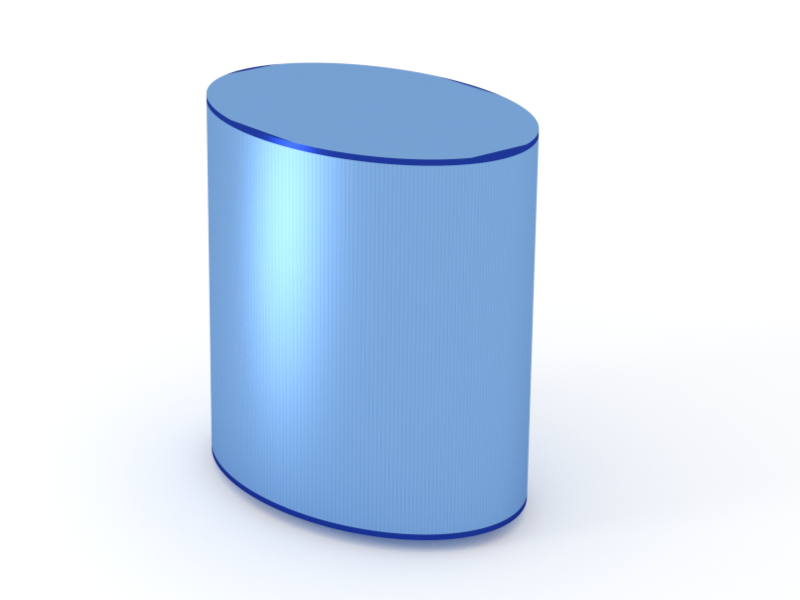
\includegraphics[width=.24\textwidth]{fig/blue/EllipsoidalCylinder3d.png}}
\hfill
\subfigure[Top view]{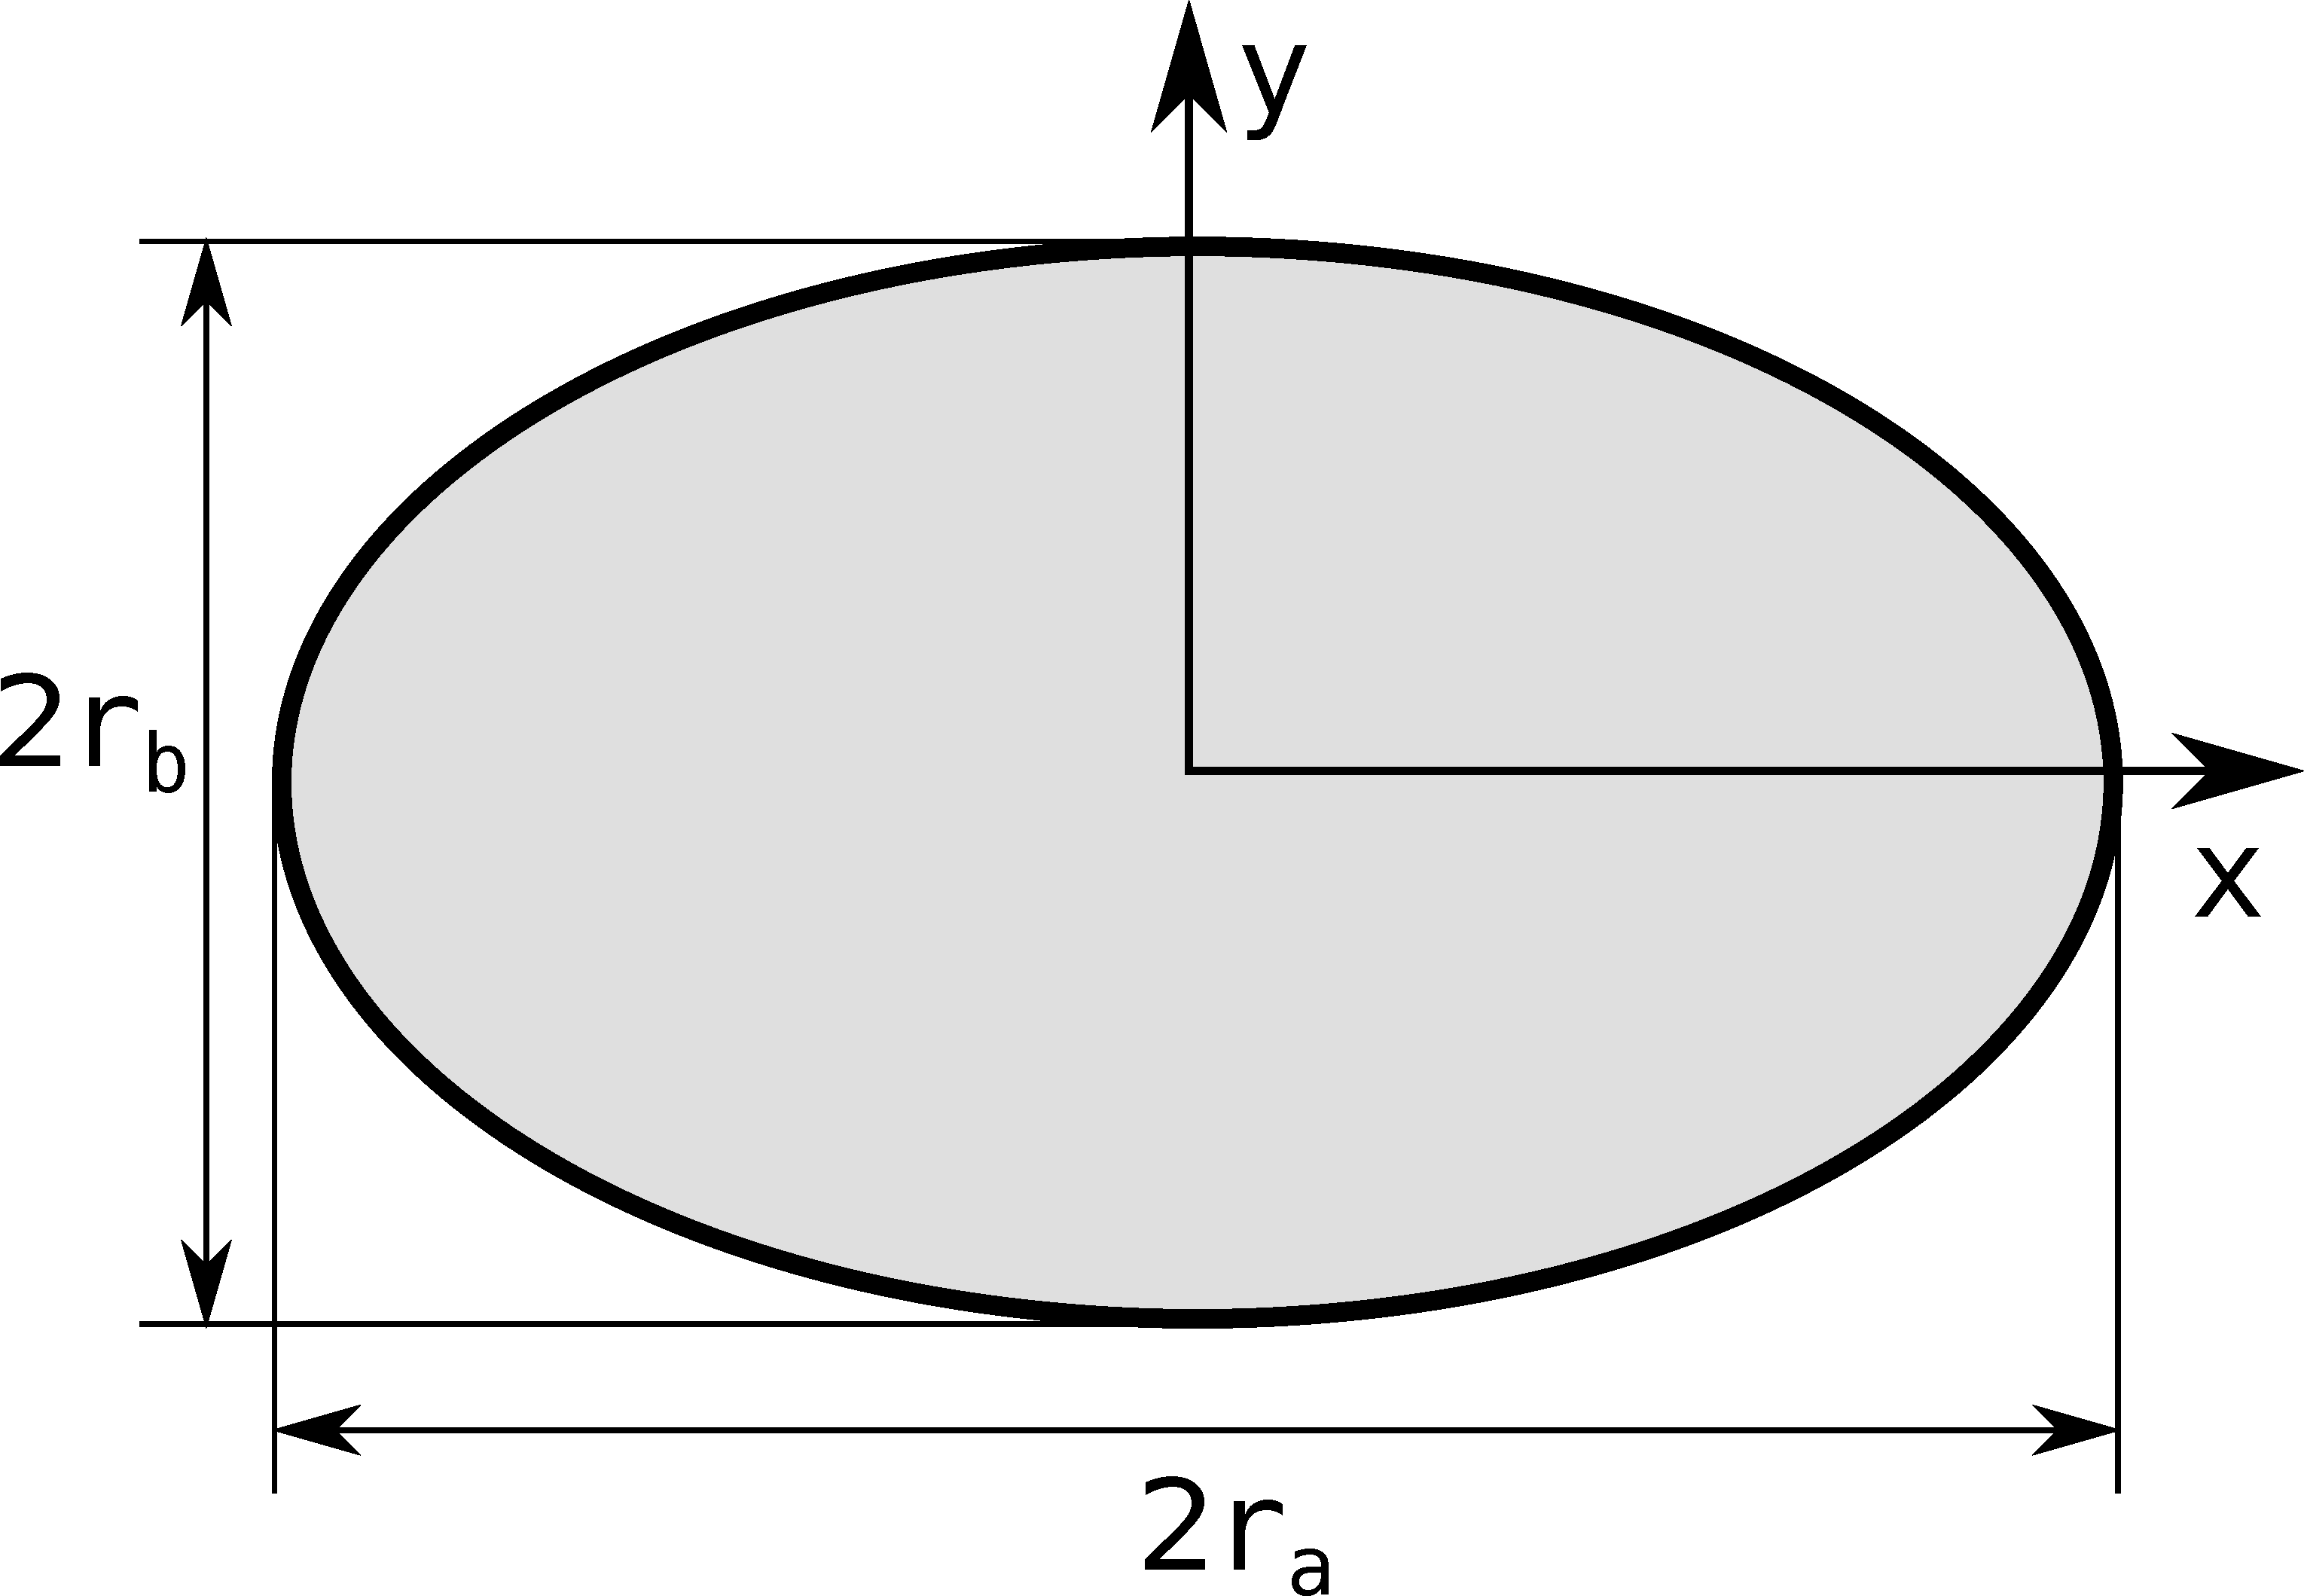
\includegraphics[width=.30\textwidth]{fig/cuts/EllipsoidalCylinder2dxy.pdf}}
\hfill
\subfigure[Side view]{\raisebox{4mm}{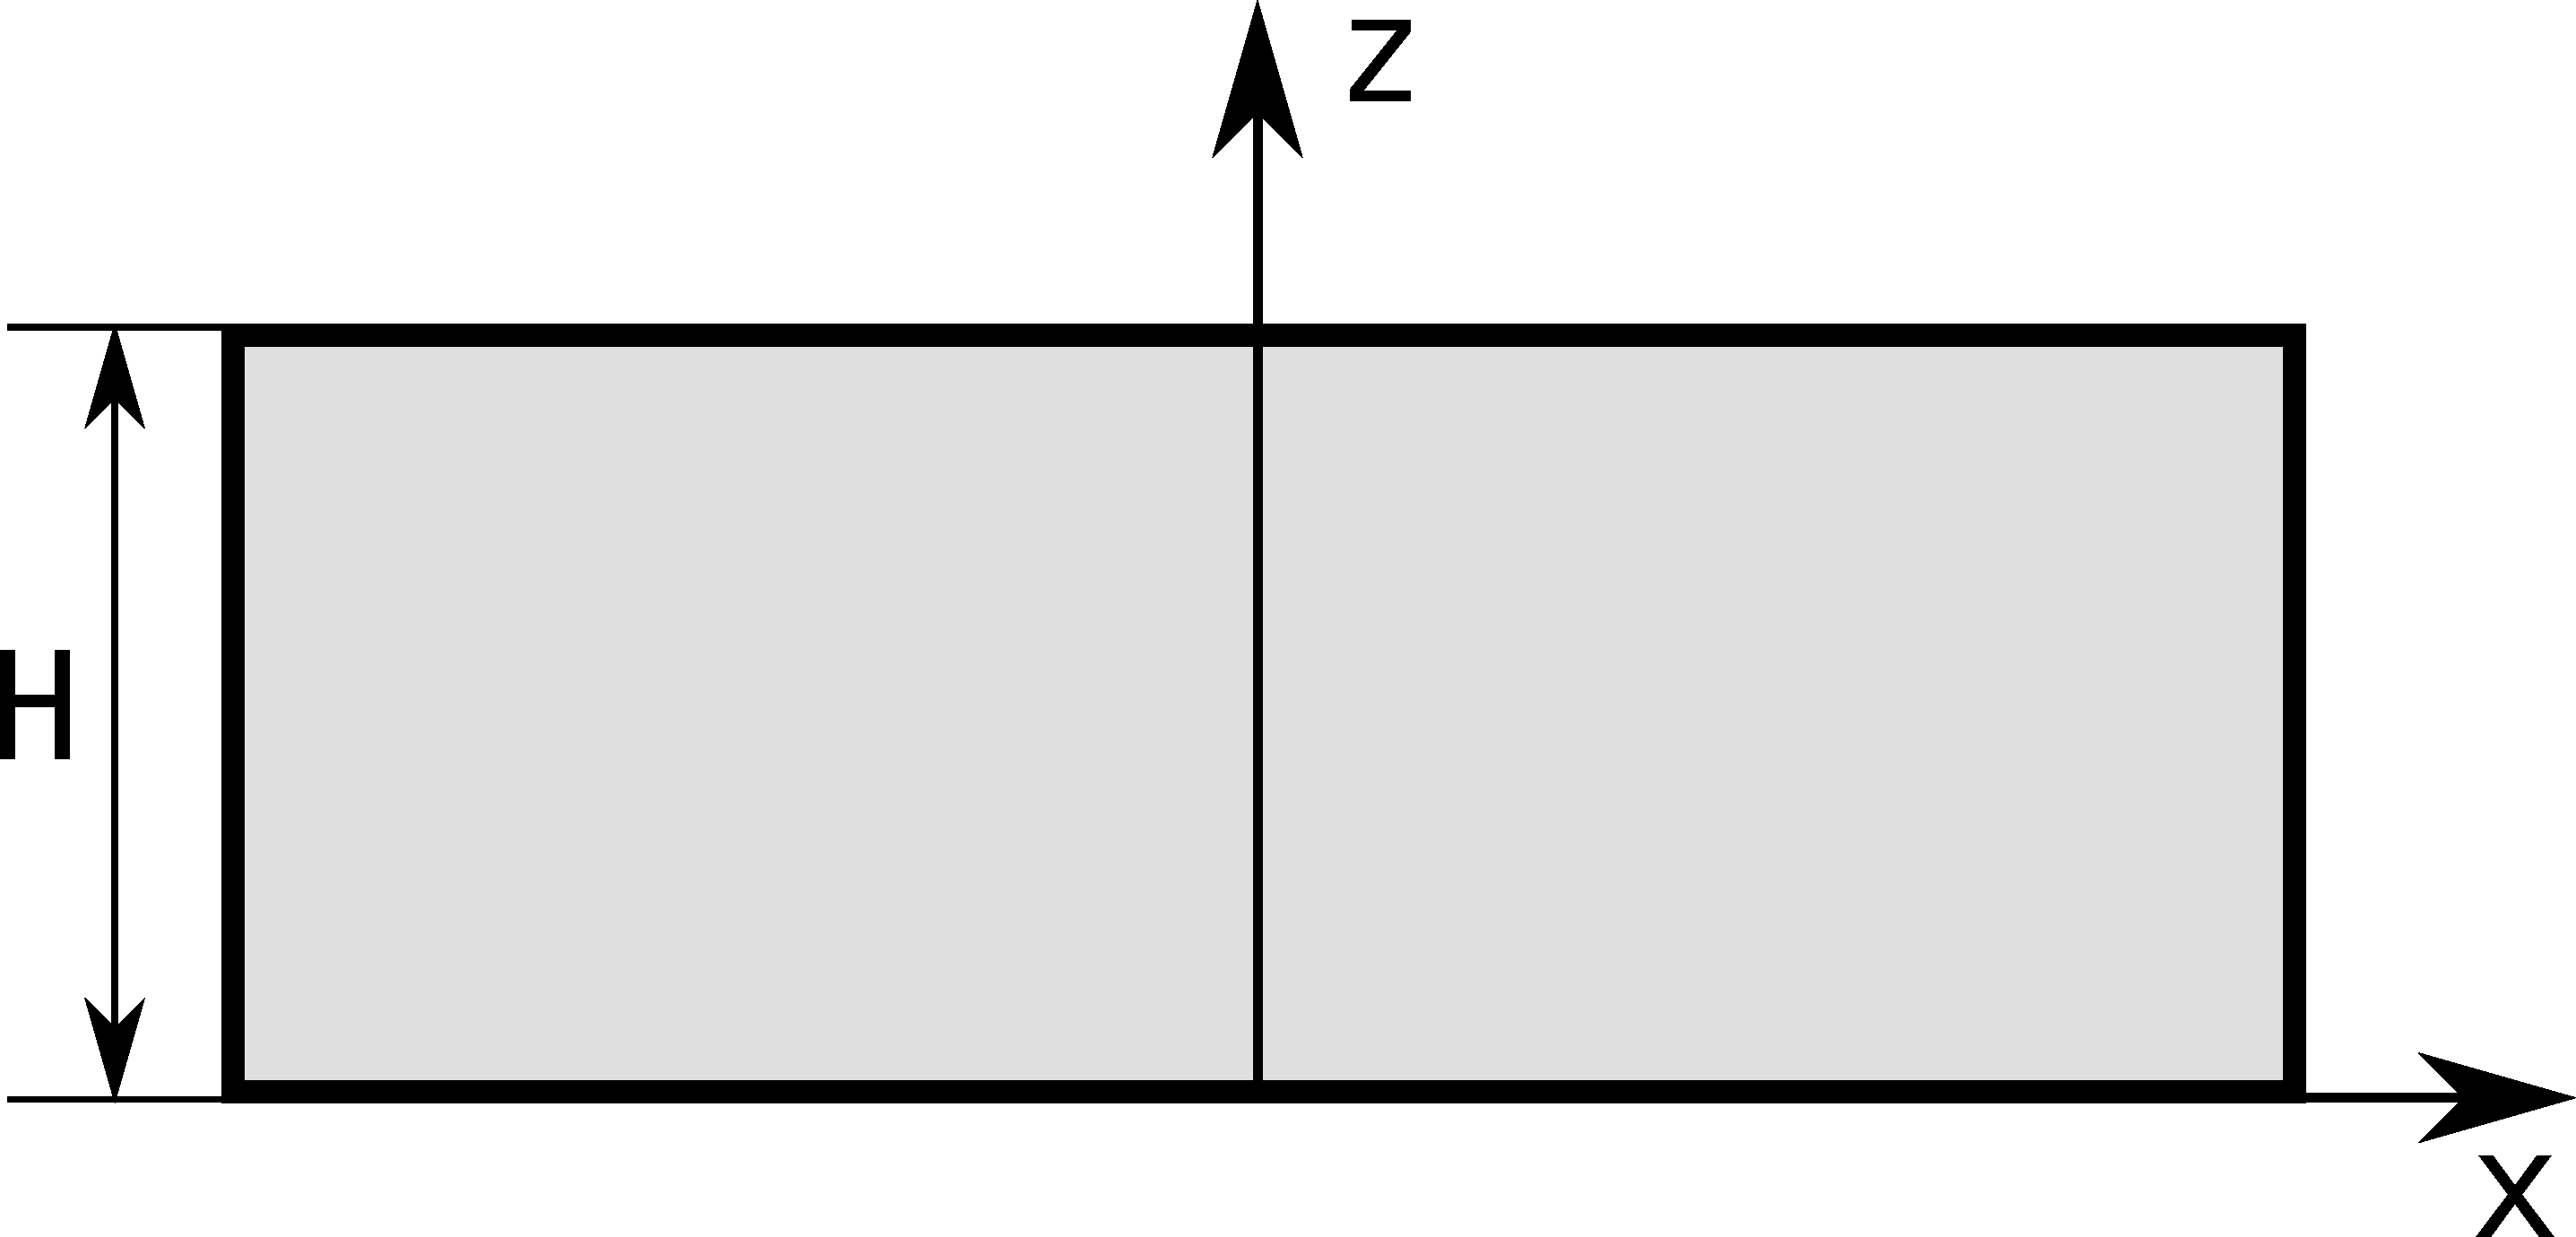
\includegraphics[width=.30\textwidth]{fig/cuts/EllipsoidalCylinder2dxz.pdf}}}
\hfill
\caption{A upright cylinder whose cross section is an ellipse.}
\end{figure}

\paragraph{Syntax and parameters}\strut\\[-2ex plus .2ex minus .2ex]
\begin{lstlisting}[language=python, style=eclipseboxed,numbers=none,nolol]
  FormFactorEllipsoidalCylinder(radius_a, radius_b, height)
\end{lstlisting}
with the parameters
\begin{itemize}
\item \texttt{radius\_a}, in $x$ direction, $R_a$,
\item \texttt{radius\_b}, in $y$ direction, $R_b$,
\item height $H$.
\end{itemize}


\paragraph{Form factor etc}\strut\\
Notation:
\begin{equation*}
  \gamma \coloneqq \sqrt{(q_x R_a)^2+(q_y R_b)^2}  
\end{equation*}
Results:
\begin{equation*}
F = 2\pi R_a R_b H \exp\left(i\frac{q_z H}{2}\right)
   \sinc\left(\frac{q_z H}{2}\right) \frac{J_1(\gamma)}{\gamma},
\end{equation*}
\begin{equation*}
  V = \pi R_a R_bH,
\end{equation*}
\begin{equation*}
  S = R_a R_b.
\end{equation*}

\paragraph{Example}\strut\\
Figure~\ref{fig:FFellipscylinderEx} shows the normalized intensity
$|F|^2/V^2$, computed with $R_a=8$~nm, $R_b=13$~nm, and $H=16$~nm.
\begin{figure}[H]
\begin{center}
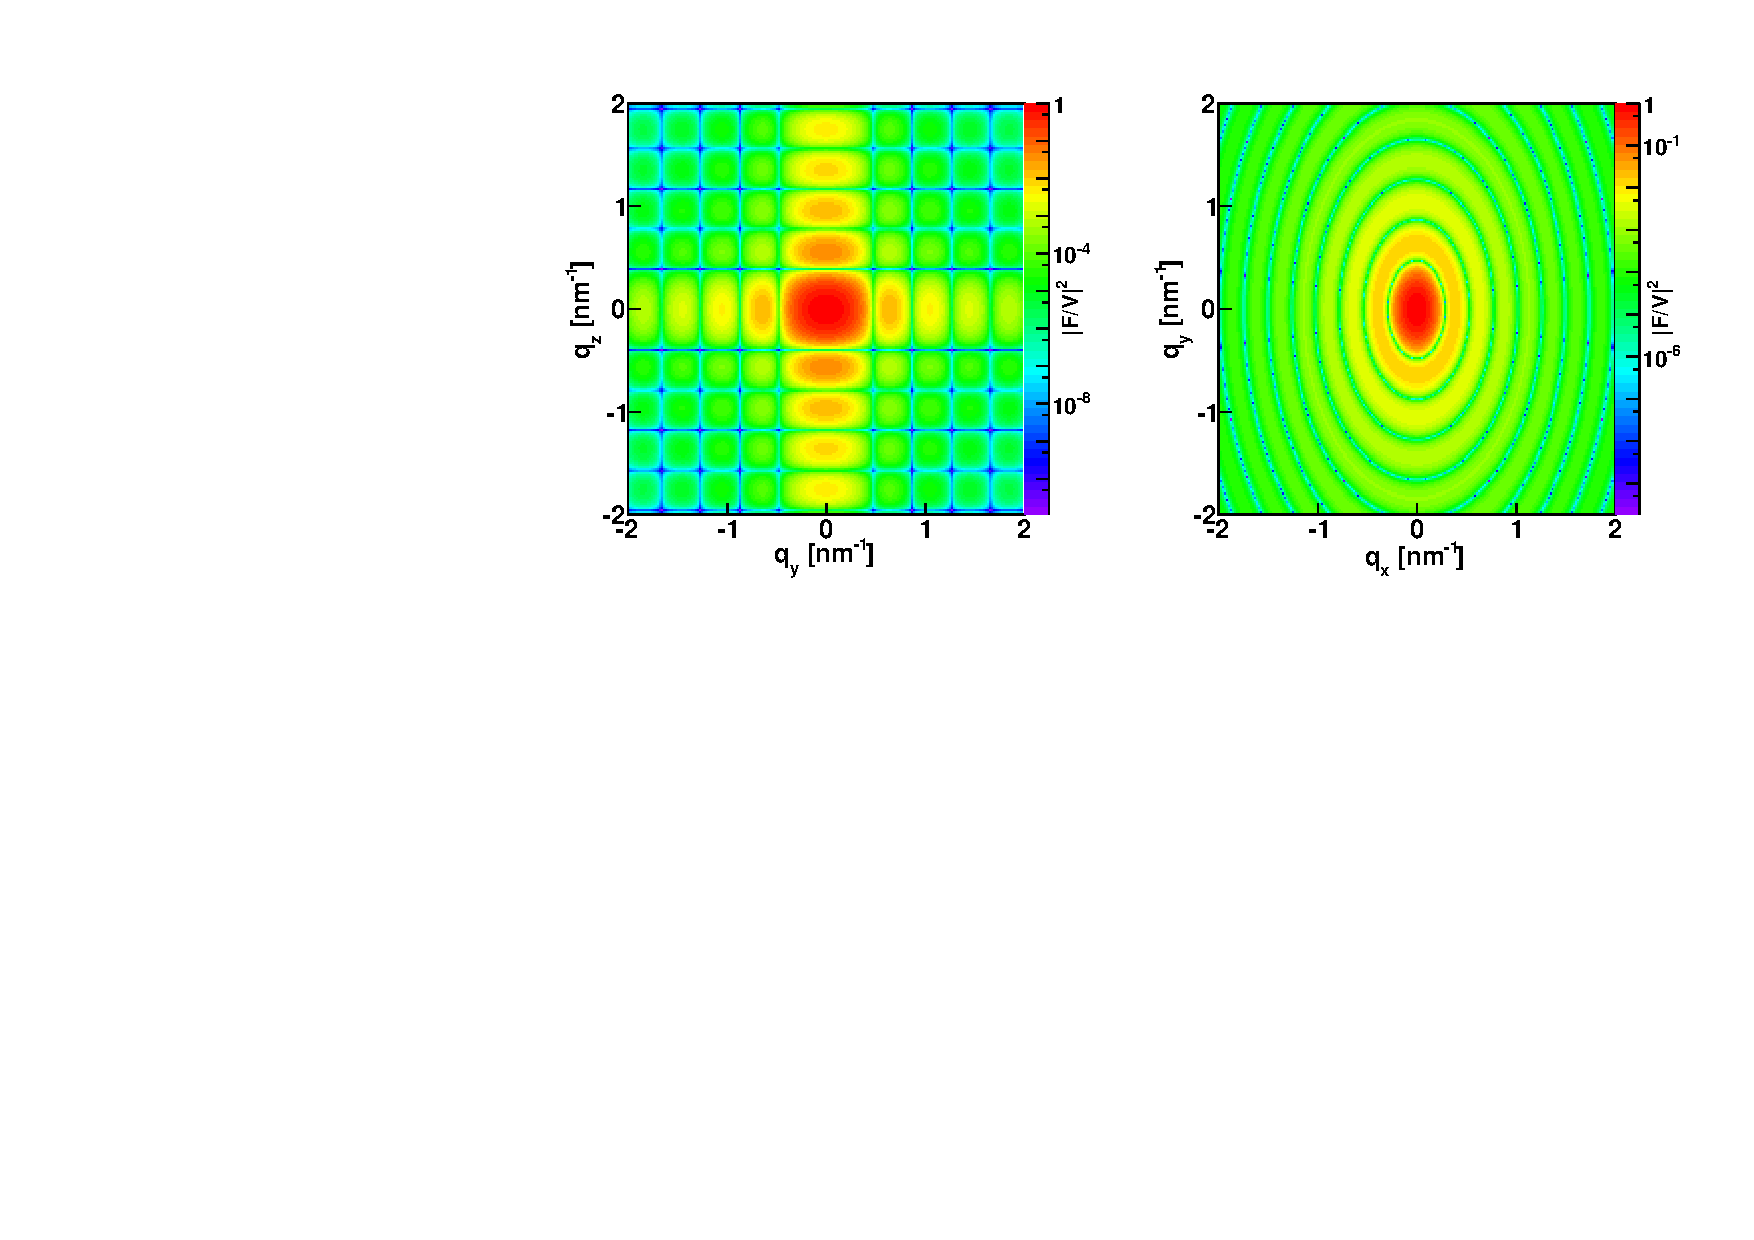
\includegraphics[angle=-90,width=\textwidth]{fig/ff/figffellipscylinder.pdf}
\end{center}
\caption{Normalized intensity for the form factor of an ellipsoidal
  cylinder plotted against ($q_y$, $q_z$) and ($q_x$,
  $q_y$) and computed with \Code{FormFactorEllipsoidalCylinder(8.*nanometer, 13.*nanometer, 16*nanometer)}.}
\label{fig:FFellipscylinderEx}
\end{figure}

\paragraph{References}\strut\\
Agrees with the \IsGISAXS\ form factor
\E{Ellipsoid} \cite[Eq.~2.41, wrongly labeled in Fig.~2.4]{Laz08}
or \E{Ellipsoidal Cylinder} \cite[Eq.~224]{ReLL09}.

%-------------------------------------------------------------------------------
\clearpage
\subsection{FullSphere} \label{sec:FullSphere}
  \index{Full sphere (form factor)}
  \index{Sphere (form factor)}
  \index{FormFactorFullSphere@\Code{FormFactorFullSphere}}
%-------------------------------------------------------------------------------

\paragraph{Real-space geometry}\strut\\

\begin{figure}[H]
\hfill
\subfigure[Perspective]{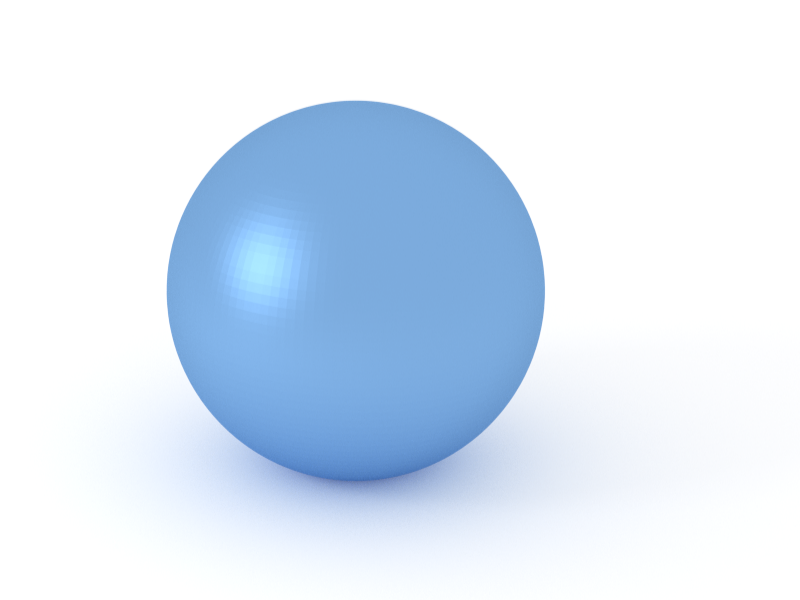
\includegraphics[width=.24\textwidth]{fig/blue/FullSphere3d.png}}
\hfill
\subfigure[Top view]{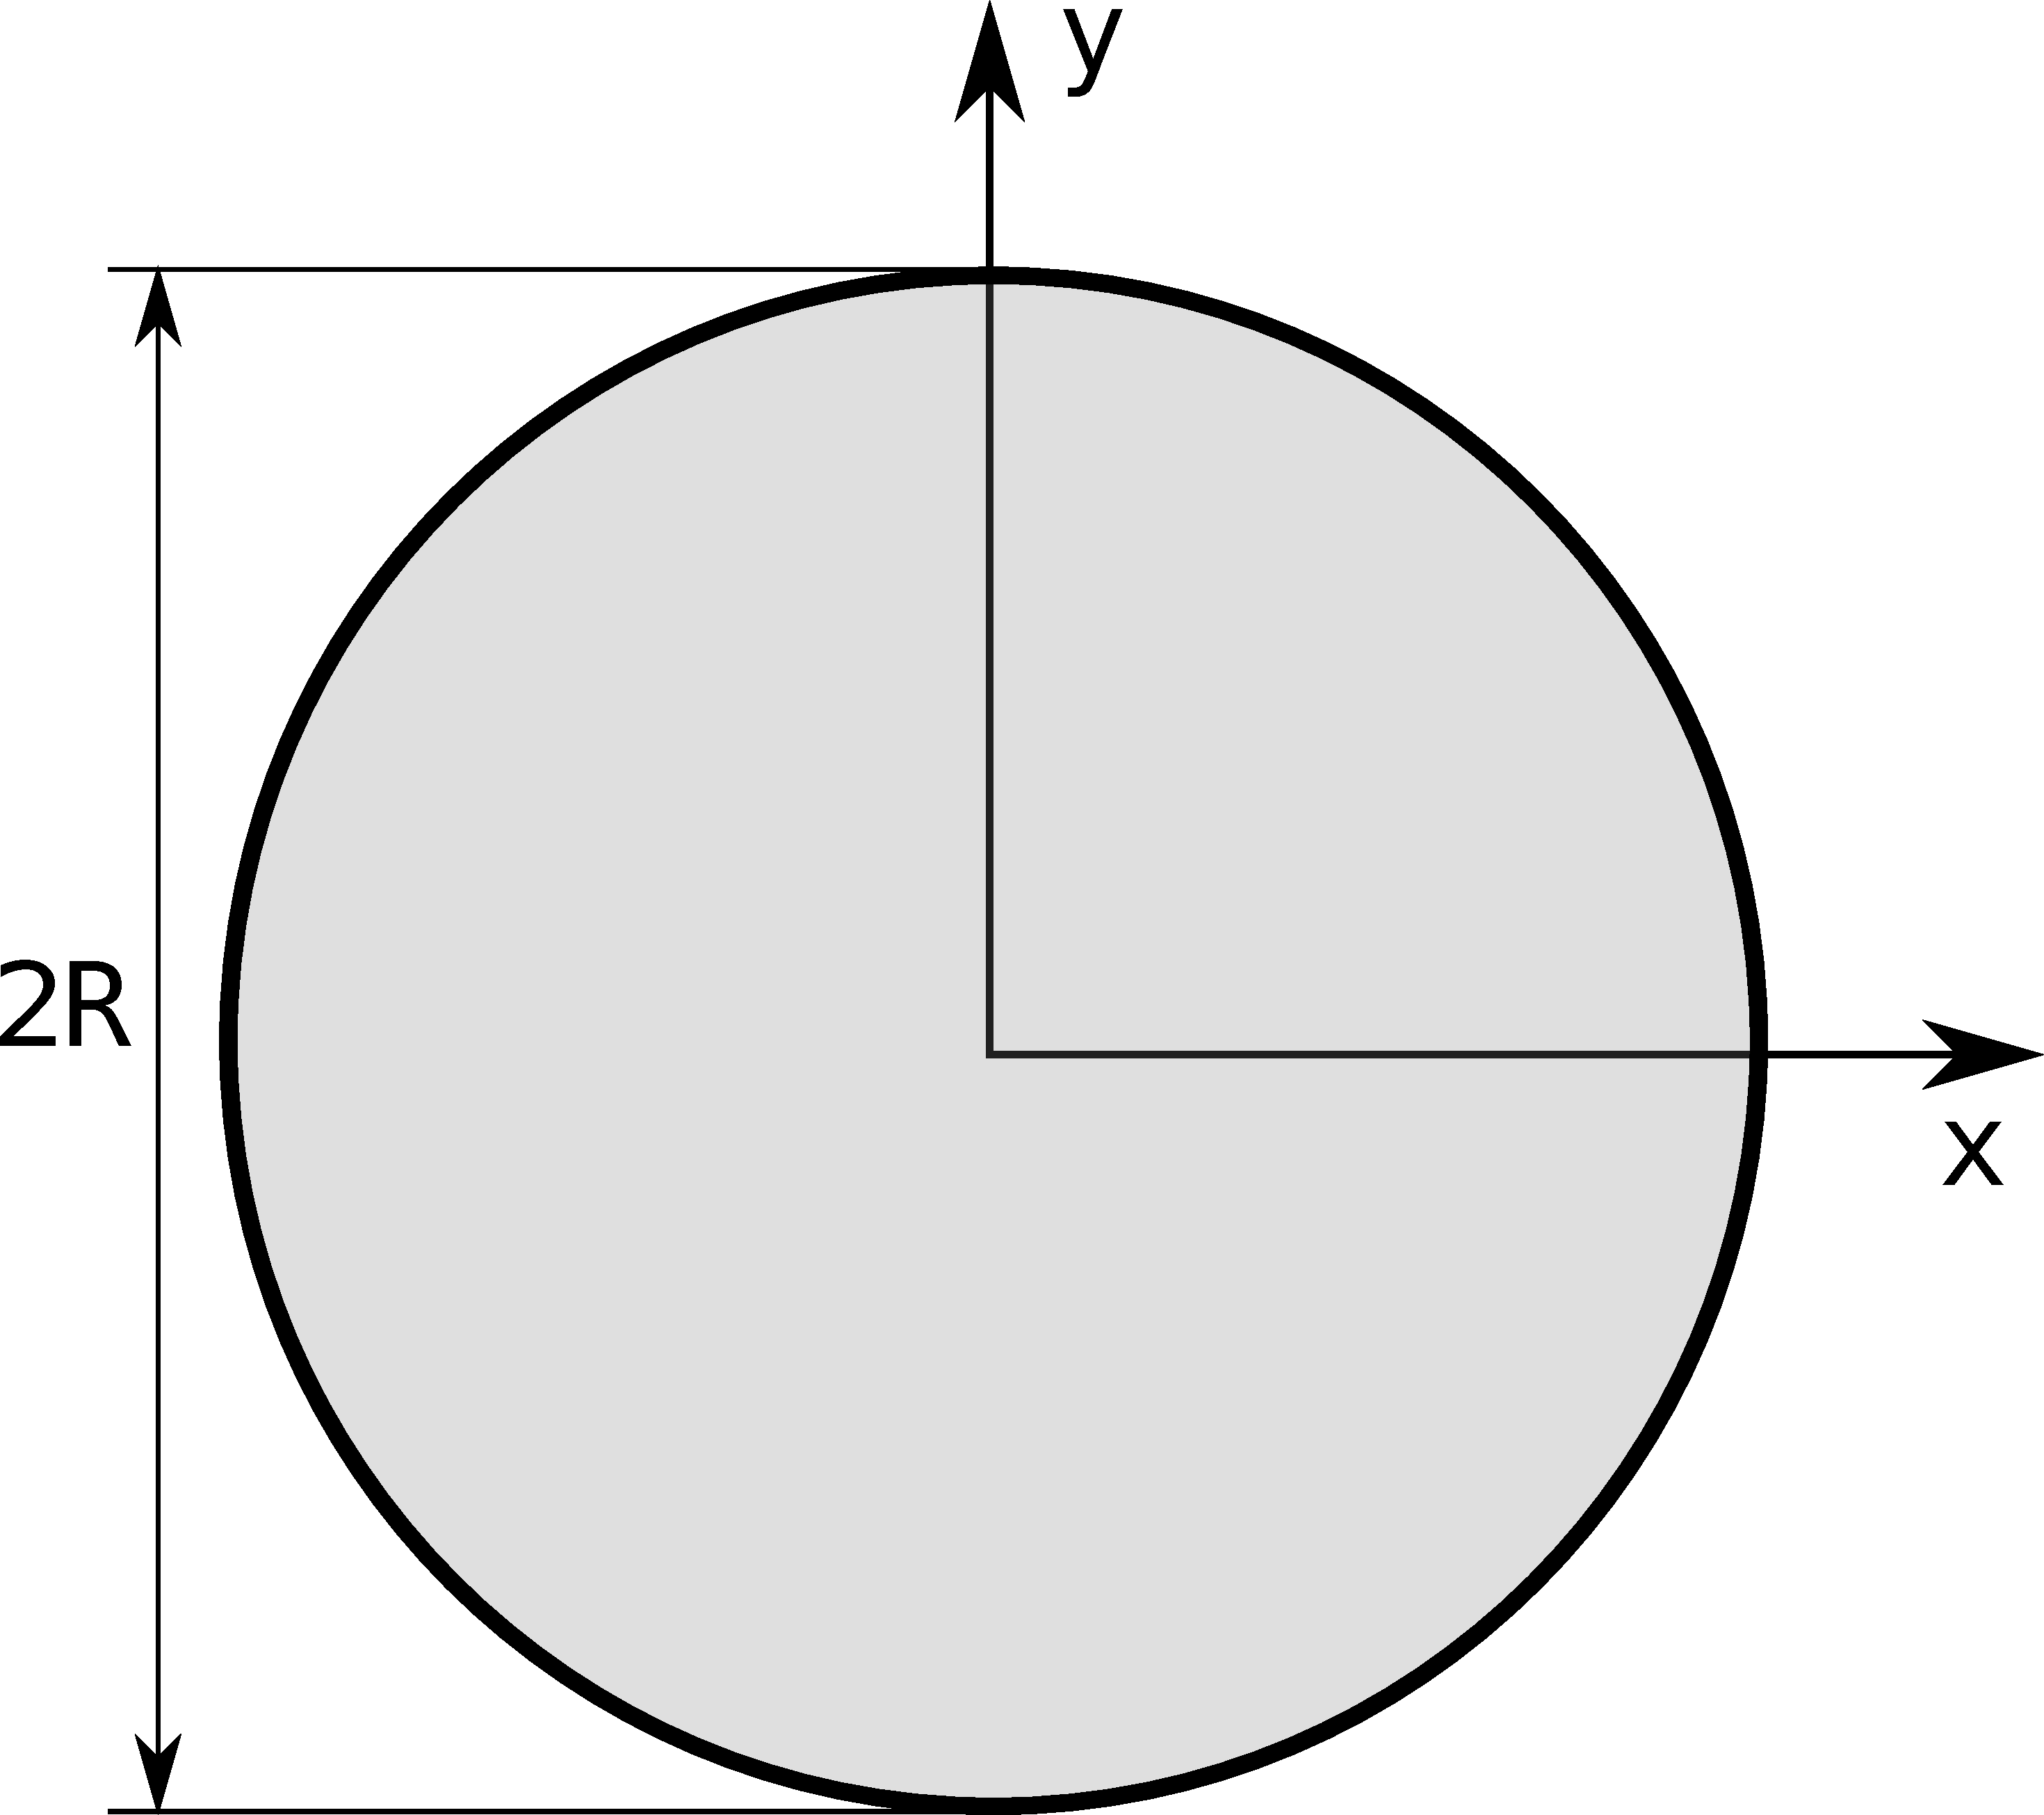
\includegraphics[width=.30\textwidth]{fig/cuts/FullSphere2dxy.pdf}}
\hfill
\subfigure[Side view]{\raisebox{-2mm}{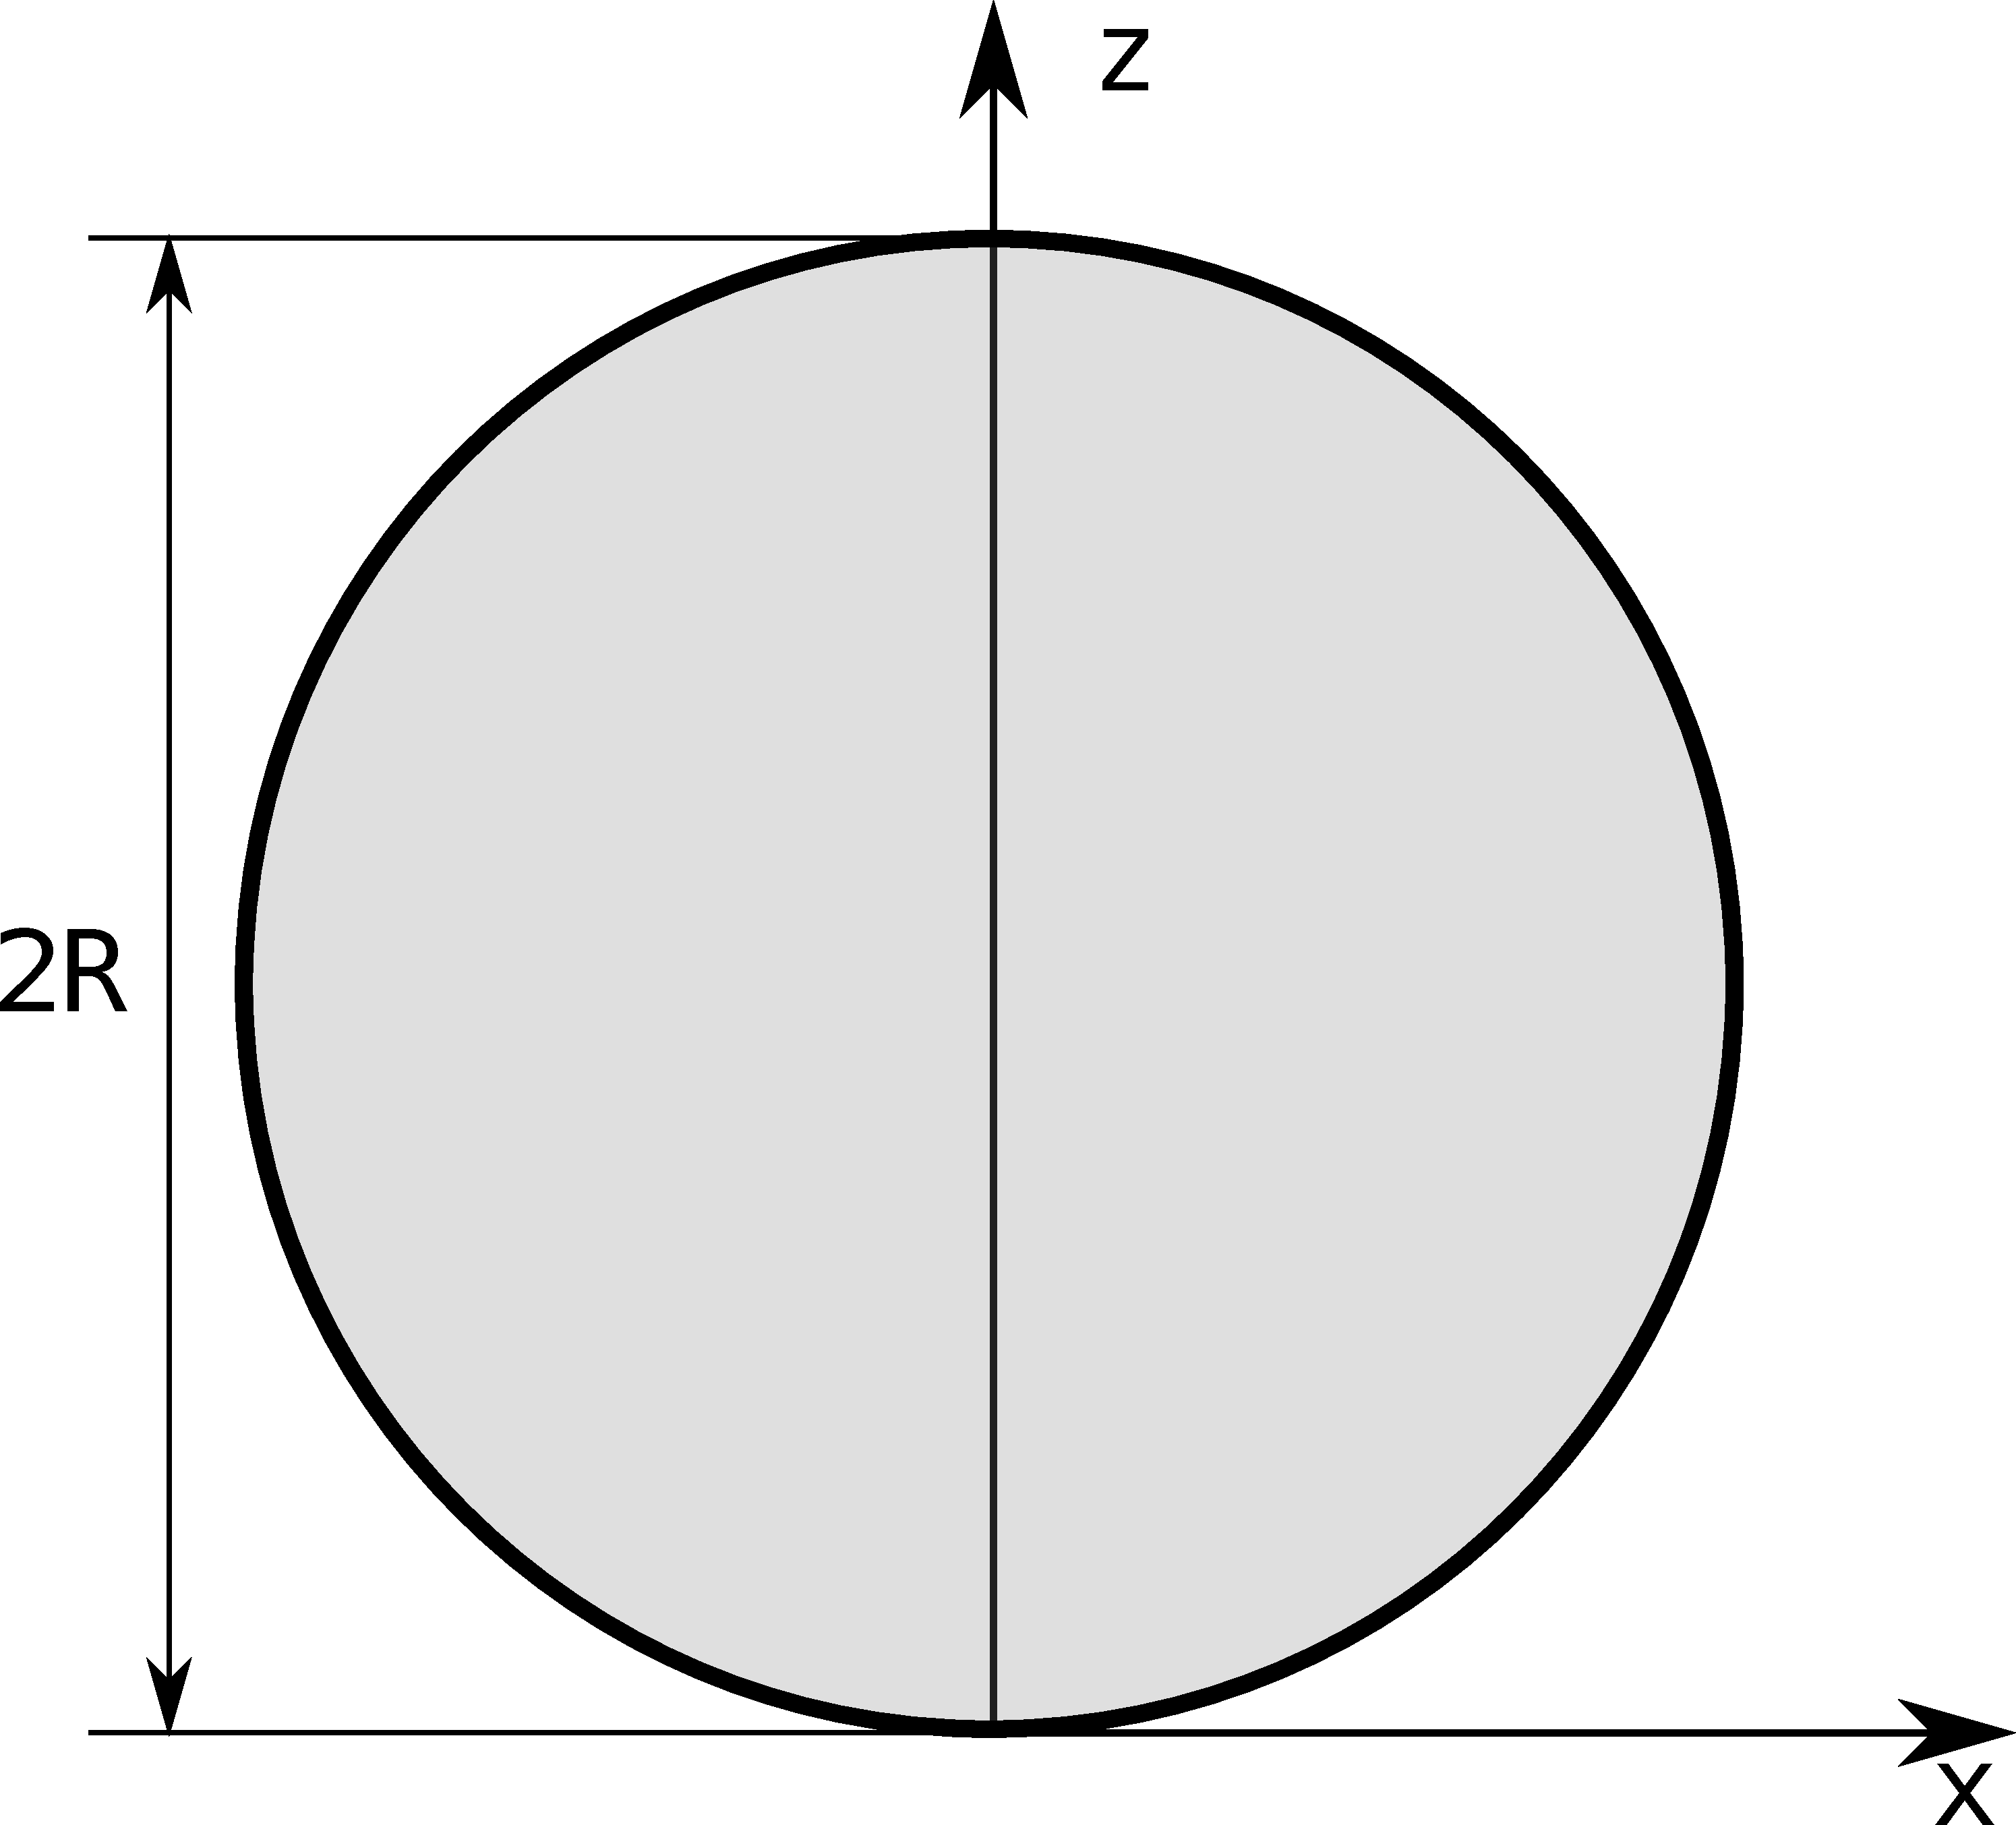
\includegraphics[width=.30\textwidth]{fig/cuts/FullSphere2dxz.pdf}}}
\hfill
\caption{A full sphere.}
\end{figure}

\FloatBarrier

\paragraph{Syntax and parameters}\strut\\[-2ex plus .2ex minus .2ex]
\begin{lstlisting}[language=python, style=eclipseboxed,numbers=none,nolol]
  FormFactorFullSphere(radius)
\end{lstlisting}
with the parameter
\begin{itemize}
\item \texttt{radius}, $R$.
\end{itemize}


\paragraph{Form factor etc}\strut\\
\begin{equation*}
F = 4\pi R^3 \exp(iq_z R)\frac{\sin(q R) - q R \cos(q R)}{(qR)^3},
\end{equation*}
\begin{equation*}
  V = \dfrac{4\pi}{3}R^3,
\end{equation*}
\begin{equation*}
  S= \pi R^2.
\end{equation*}

\paragraph{Example}\strut\\
Figure~\ref{fig:FFfSphereEx} shows the normalized intensity $|F|^2/V^2$, computed with $R=8$~nm.
\begin{figure}[H]
\begin{center}
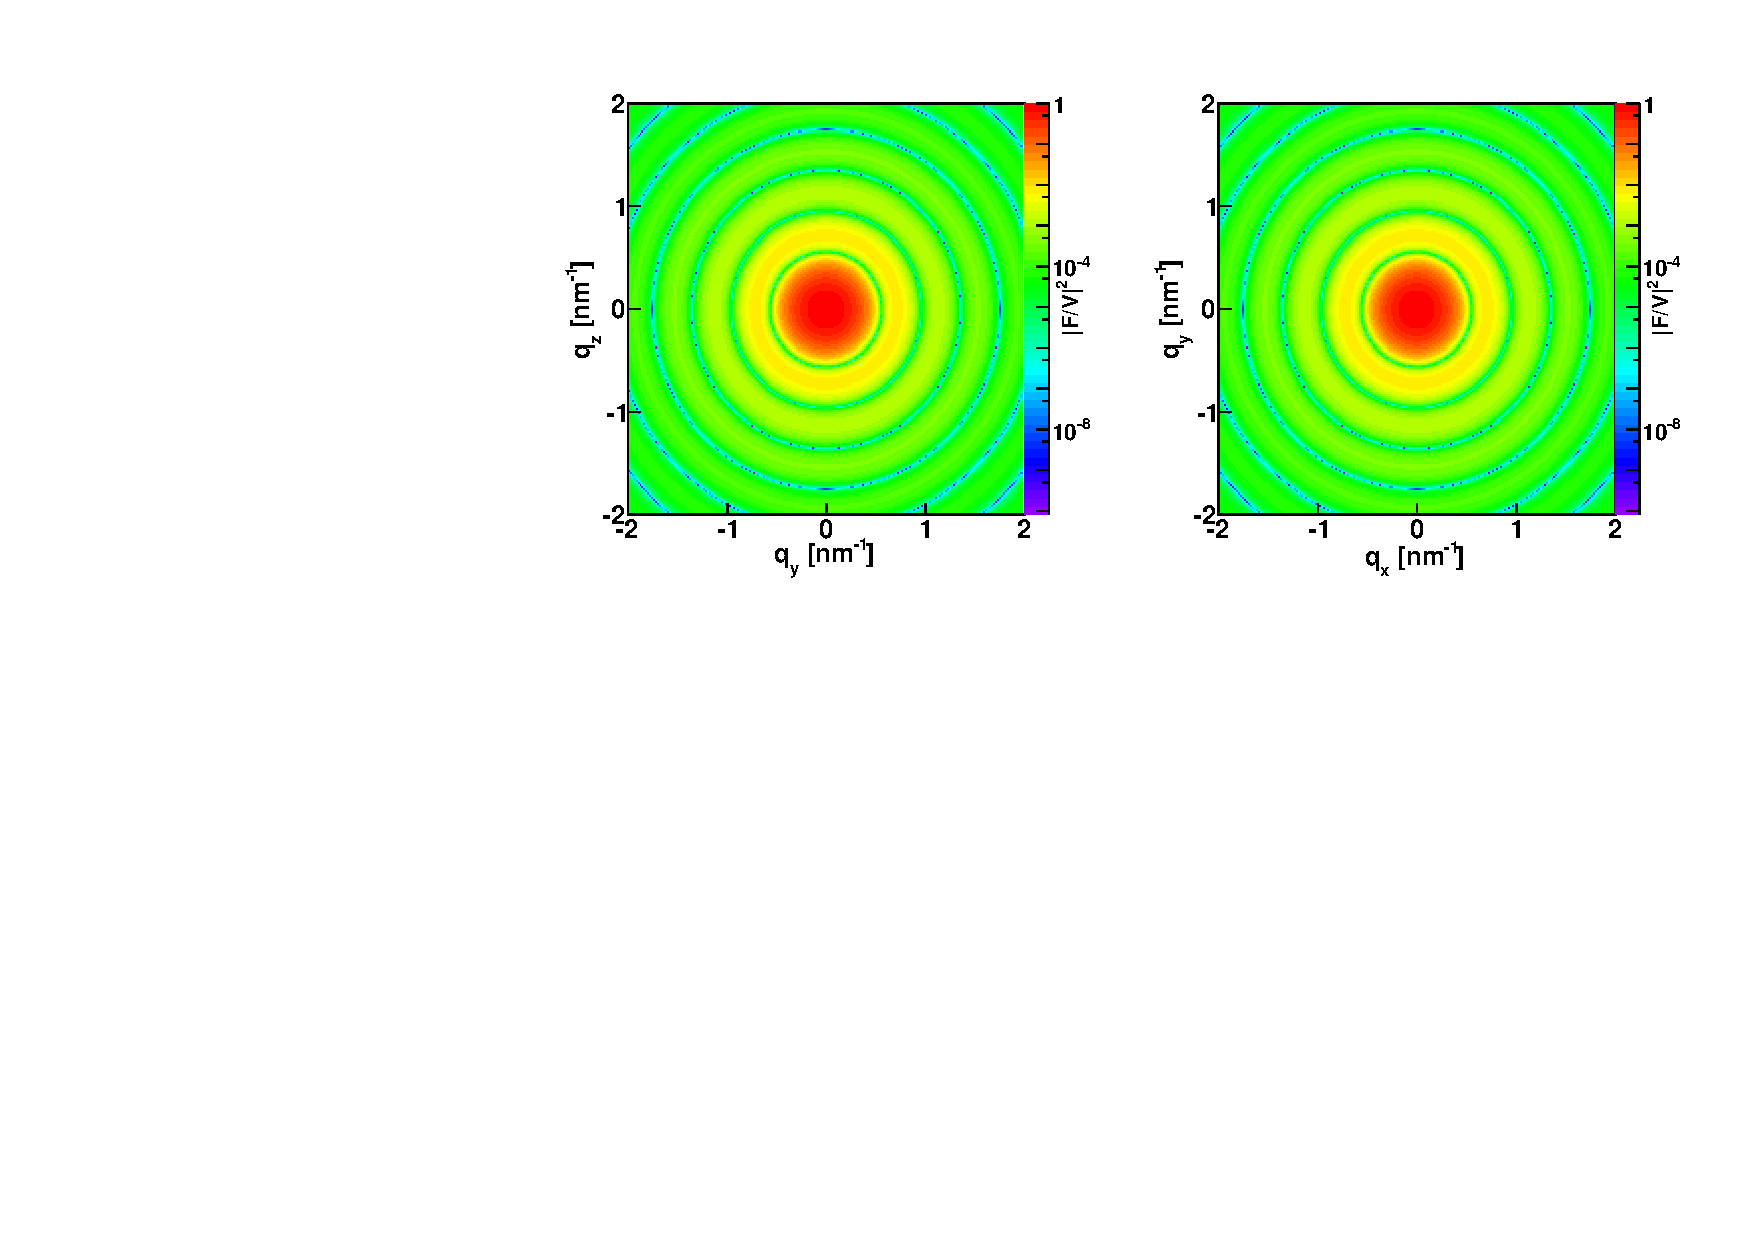
\includegraphics[angle=-90,width=\textwidth]{fig/ff/figfffsphere.pdf}
\end{center}
\caption{Normalized intensity for the
  form factor of a Full Sphere plotted against ($q_y$, $q_z$) and ($q_x$, $q_y$) and computed with \Code{FormFactorFullSphere(8.*nanometer)}.}
\label{fig:FFfSphereEx}
\end{figure}

\paragraph{References}\strut\\
This form factor, which certainly goes back at least to Lord Rayleigh,
agrees with the \E{Full sphere} of \IsGISAXS
\cite[Eq.~2.36]{Laz08} \cite[Eq.~226]{ReLL09}.

%-------------------------------------------------------------------------------
\clearpage
\subsection{HemiEllipsoid} \label{sec:HemiEllipsoid}  
  \index{Hemi ellipsoid (form factor)}
  \index{Ellipsoid (form factor)!truncated}
  \index{Truncated ellipsoid (form factor)}
  \index{FormFactorHemiEllipsoid@\Code{FormFactorHemiEllipsoid}}
%-------------------------------------------------------------------------------

\paragraph{Real-space geometry}\strut\\

\begin{figure}[H]
\hfill
\subfigure[Perspective]{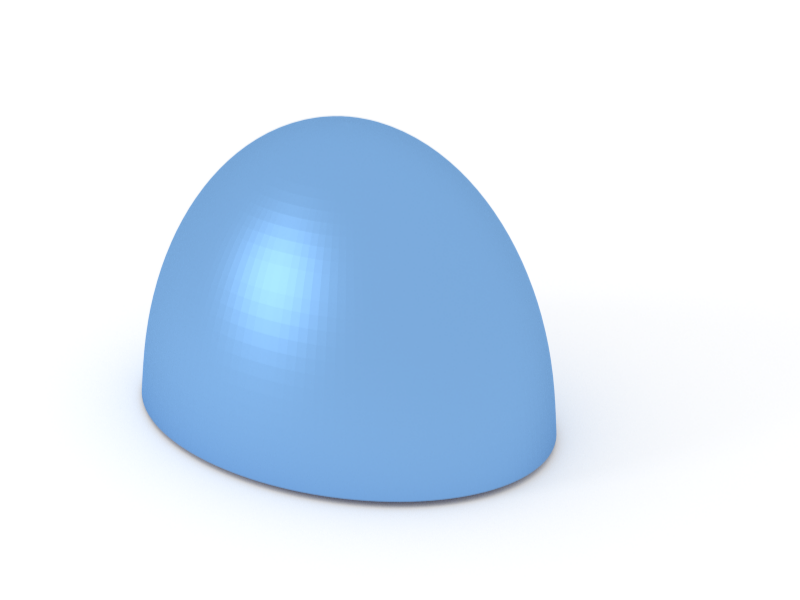
\includegraphics[width=.24\textwidth]{fig/blue/HemiEllipsoid3d.png}}
\hfill
\subfigure[Top view]{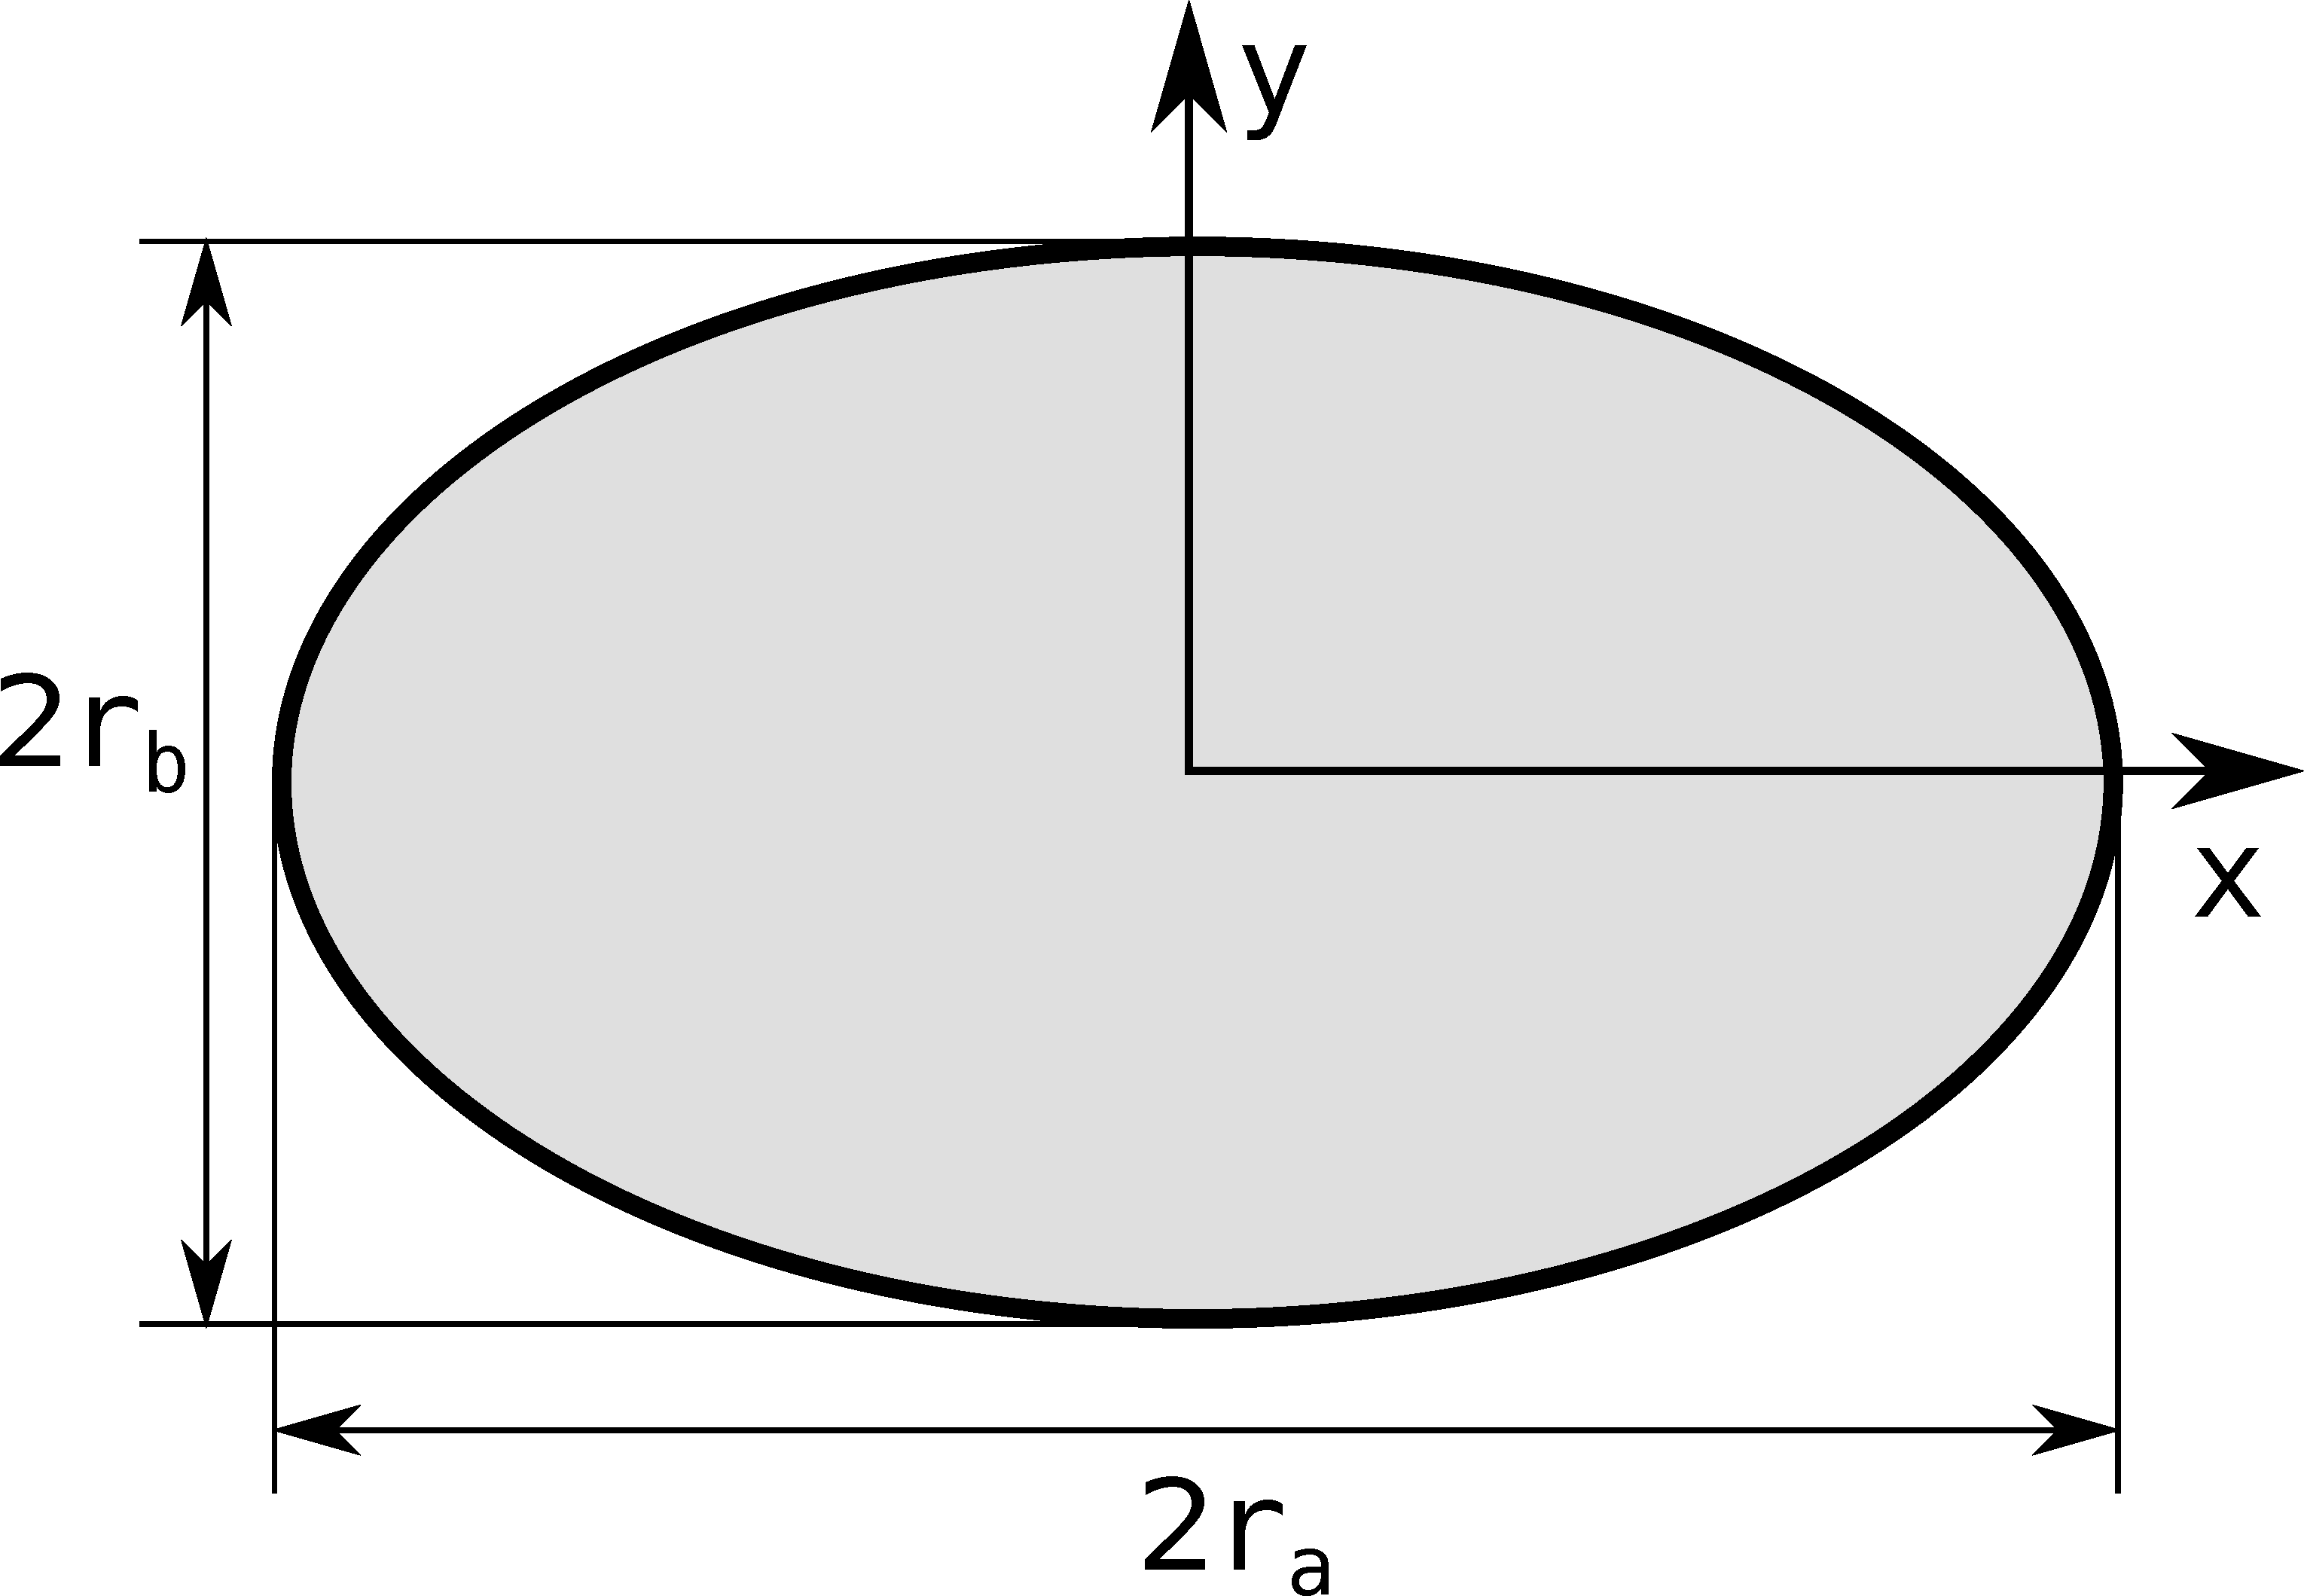
\includegraphics[width=.30\textwidth]{fig/cuts/HemiEllipsoid2dxy.pdf}}
\hfill
\subfigure[Side view]{\raisebox{5mm}{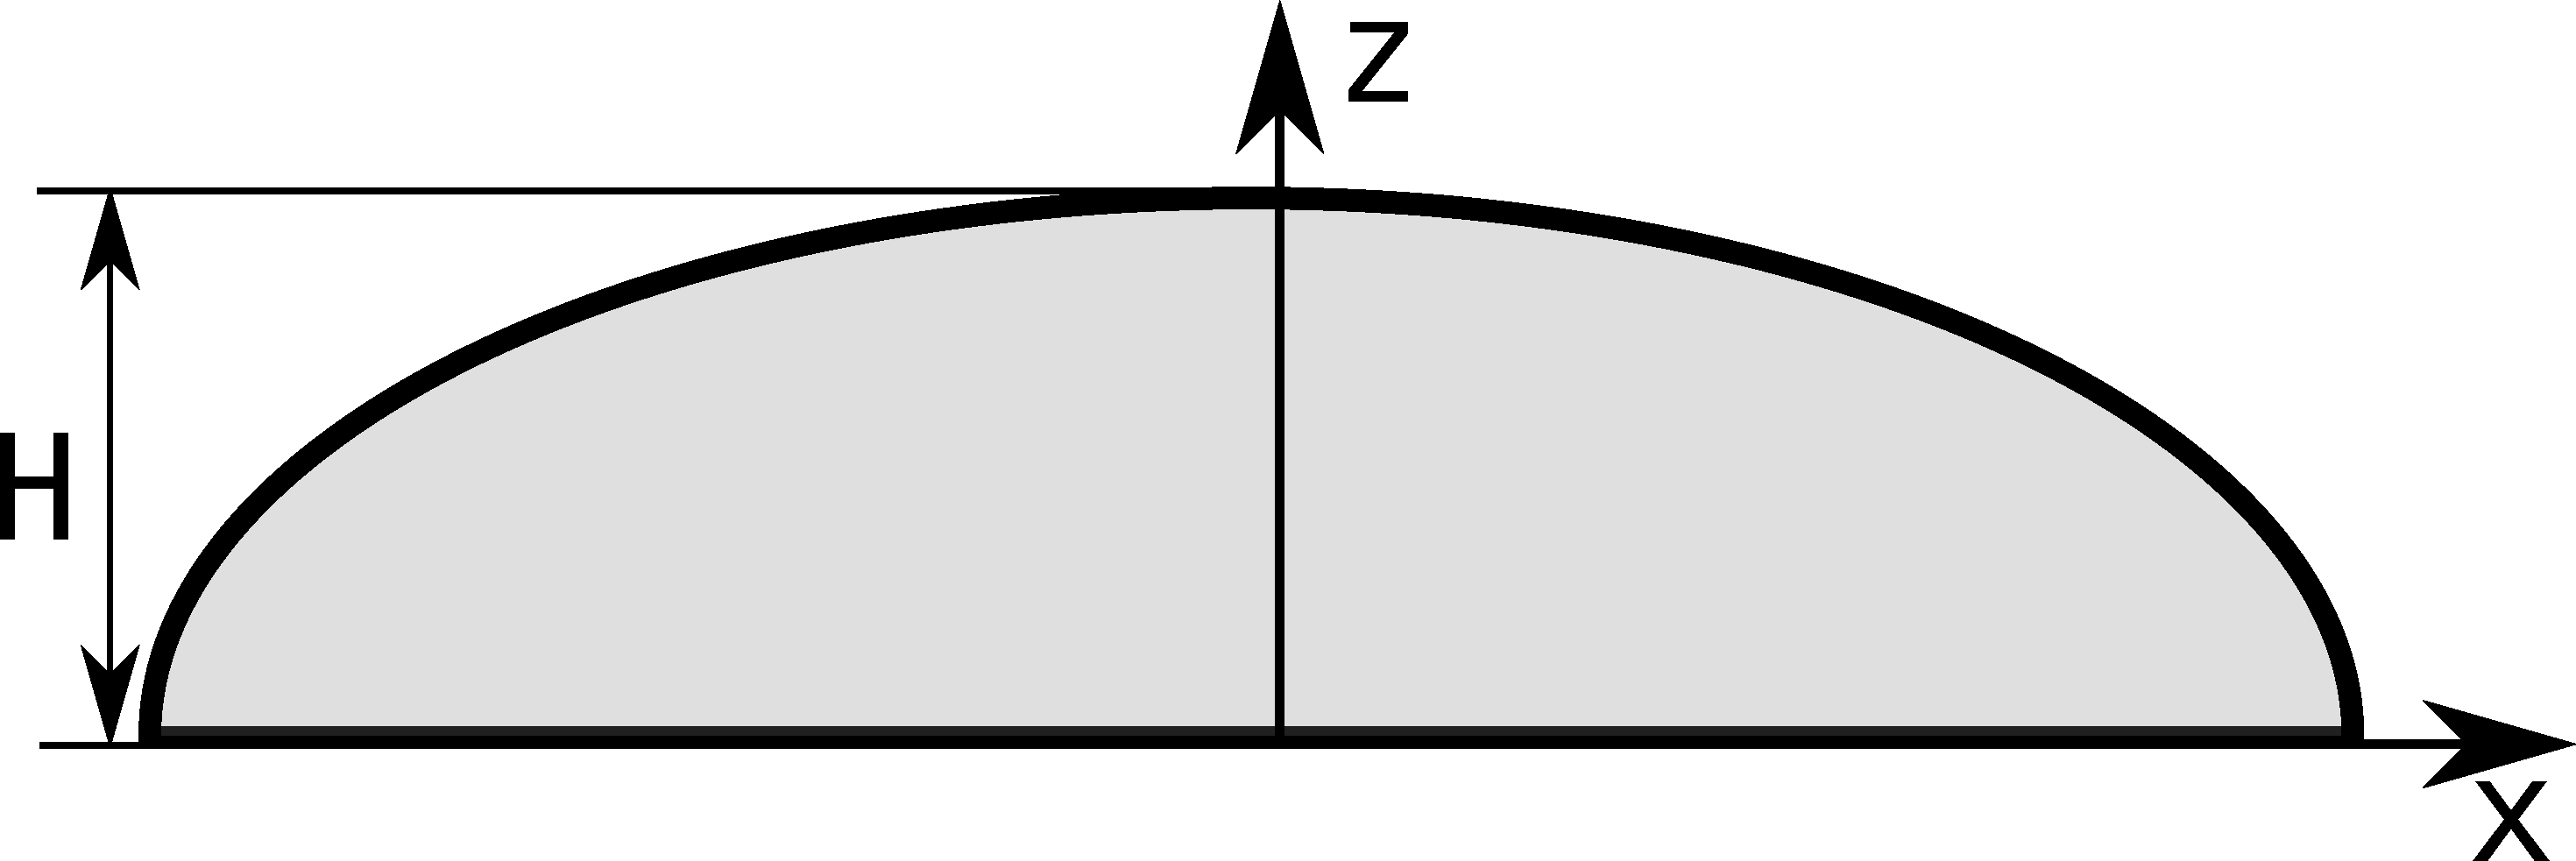
\includegraphics[width=.30\textwidth]{fig/cuts/HemiEllipsoid2dxz.pdf}}}
\hfill
\caption{An horizontally oriented ellipsoid, truncated at the central plane.}
\end{figure}

\paragraph{Syntax and parameters}\strut\\[-2ex plus .2ex minus .2ex]
\begin{lstlisting}[language=python, style=eclipseboxed,numbers=none,nolol]
  FormFactorHemiEllipsoid(radius_a, radius_b, height)
\end{lstlisting}
with the parameters
\begin{itemize}
\item \texttt{radius\_a}, in $x$ direction, $R_a$,
\item \texttt{radius\_b}, in $y$ direction, $R_b$,
\item \texttt{height}, equal to radius in $z$ direction, $H$
\end{itemize}


\paragraph{Form factor etc}\strut\\
Notation:
\begin{equation*}
 r_{a,z} \coloneqq R_a \sqrt{1-\left(\dfrac{z}{H} \right)^2},\quad
 r_{b,z} \coloneqq R_b \sqrt{1-\left(\dfrac{z}{H} \right)^2}, \quad
 \gamma_z =\sqrt{(q_x r_{a,z})^2+(q_y r_{b,z})^2}.
\end{equation*}
Results:
\begin{equation*}
  F = 2\pi \int_0^{H} \!\d z\, r_{a,z} r_{b,z}
                               \frac{J_1(\gamma_z)}{\gamma_z}\exp(iq_z z),
\end{equation*}
\begin{equation*}
  V = \dfrac{2}{3}\pi R_a R_bH,
\end{equation*}
\begin{equation*}
  S =\pi R_a R_b.
\end{equation*}

\paragraph{Example}\strut\\
Figure~\ref{fig:FFhemiellipsEx} shows the normalized intensity
$|F|^2/V^2$, computed with $R_a=10$~nm, $R_b=6$~nm and $H=8$~nm.

\begin{figure}[H]
\begin{center}
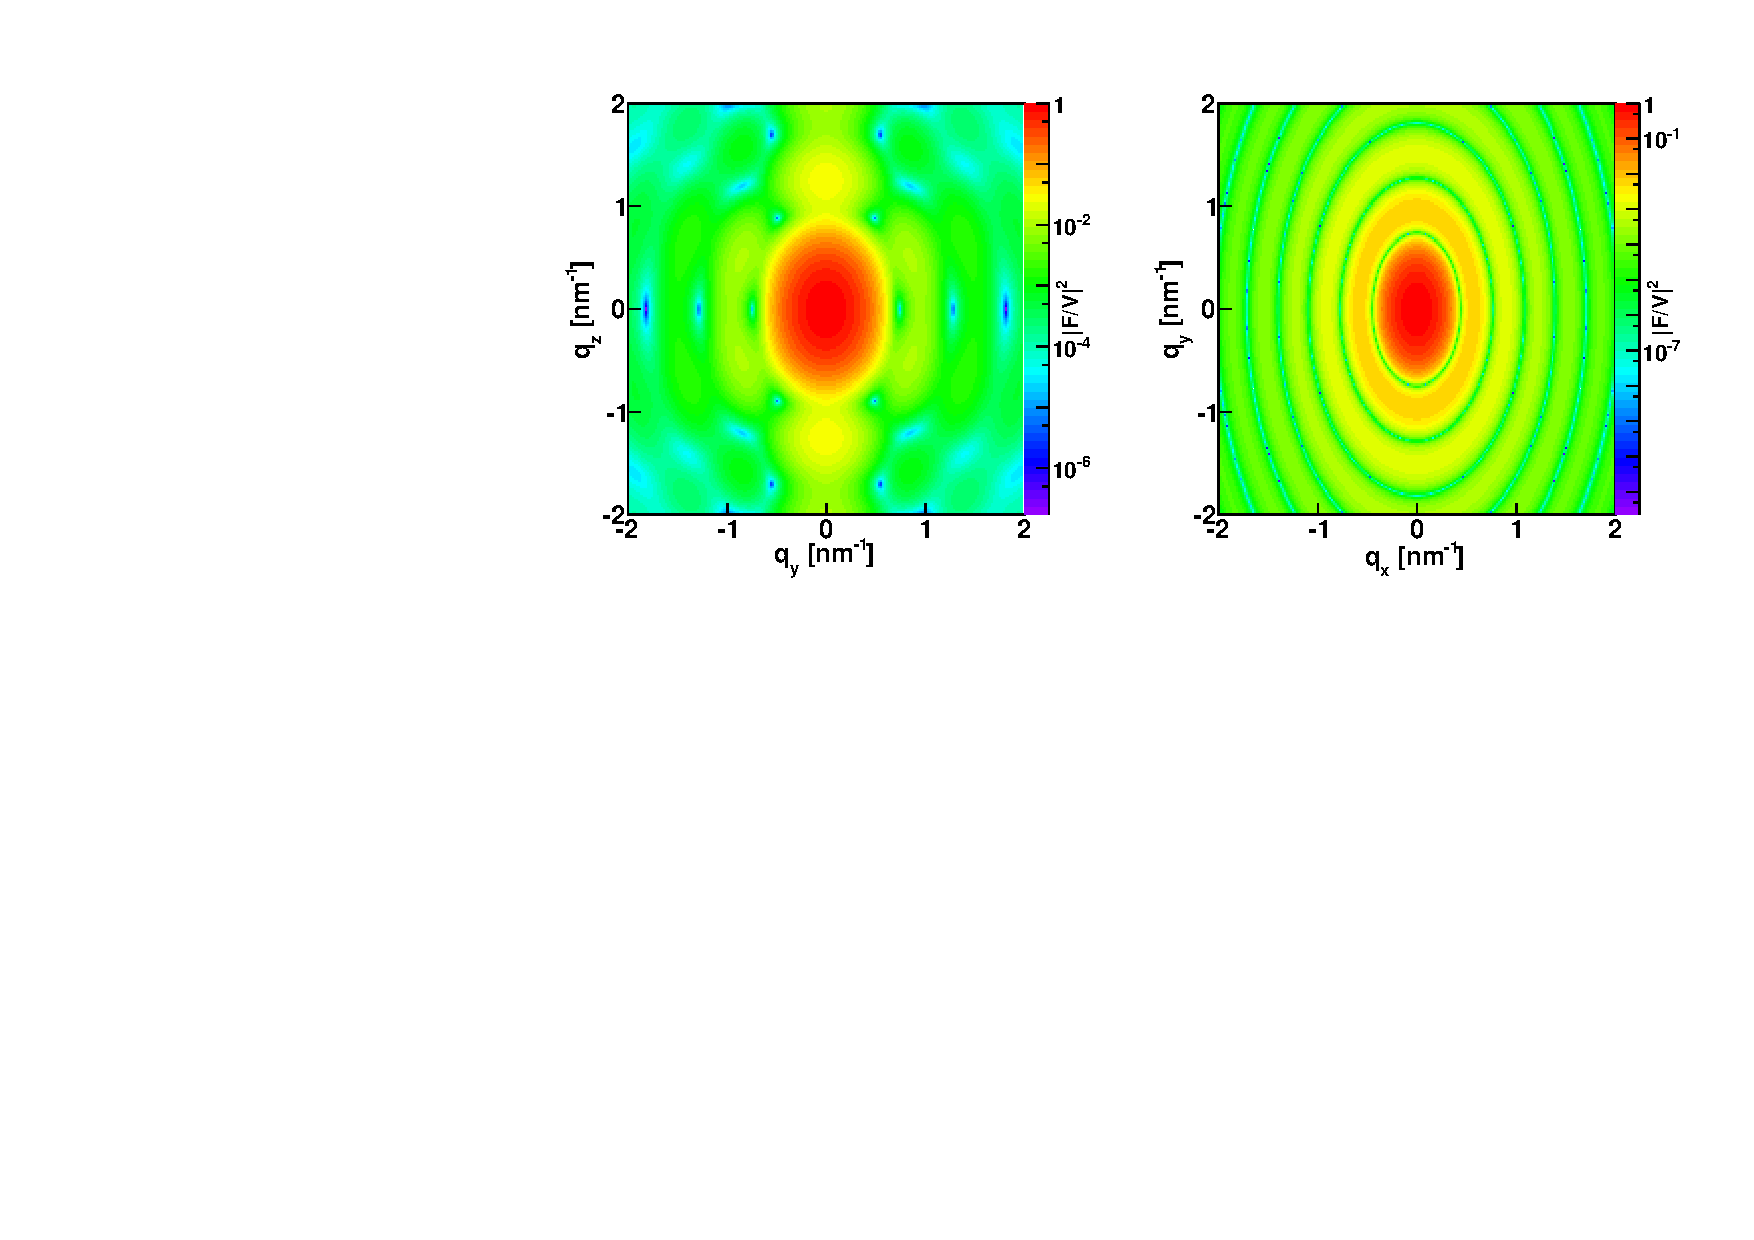
\includegraphics[angle=-90,width=\textwidth]{fig/ff/figffhemiellips.pdf}
\end{center}
\caption{Normalized intensity for the form factor of an Hemi-Ellipsoid plotted against ($q_y$, $q_z$) and  ($q_x$, $q_y$)
  computed with \Code{FormFactorHemiEllipsoid(10.*nanometer, 6.*nanometer, 8.*nanometer)}.}
\label{fig:FFhemiellipsEx}
\end{figure}

\paragraph{References}\strut\\
Agrees with the \IsGISAXS\ form factor
\E{Anisotropic hemi-ellipsoid}
\cite[Eq.~2.42, with wrong sign in the $z$-dependent phase factor]{Laz08}
or \E{Hemi-spheroid} \cite[Eq.~229]{ReLL09}.

%-------------------------------------------------------------------------------
\clearpage
\subsection{FullSpheroid} \label{sec:FullSpheroid}
  \index{Full spheroid (form factor)}
  \index{Spheroid (form factor)}
  \index{FormFactorFullSpheroid@\Code{FormFactorFullSpheroid}}
%-------------------------------------------------------------------------------

\paragraph{Real-space geometry}\strut\\

\begin{figure}[H]
\hfill
\subfigure[Perspective]{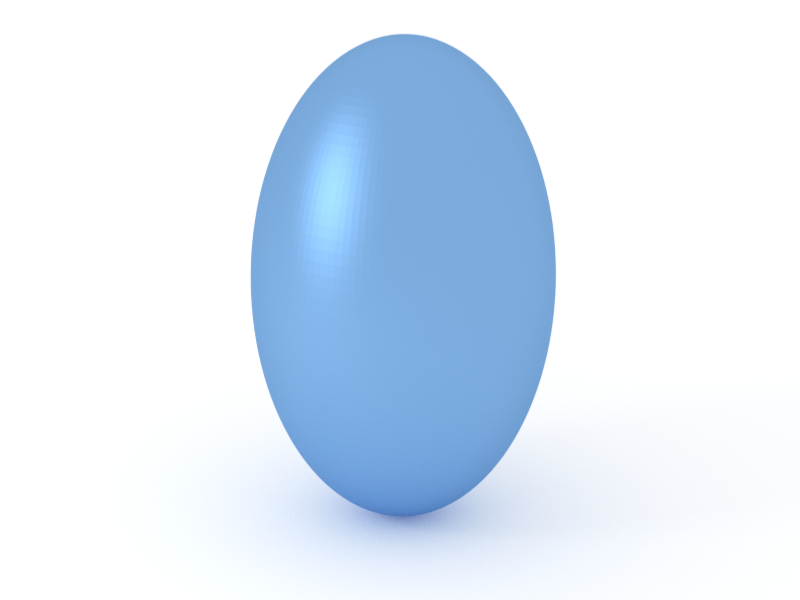
\includegraphics[width=.24\textwidth]{fig/blue/FullSpheroid3d.png}}
\hfill
\subfigure[Top view]{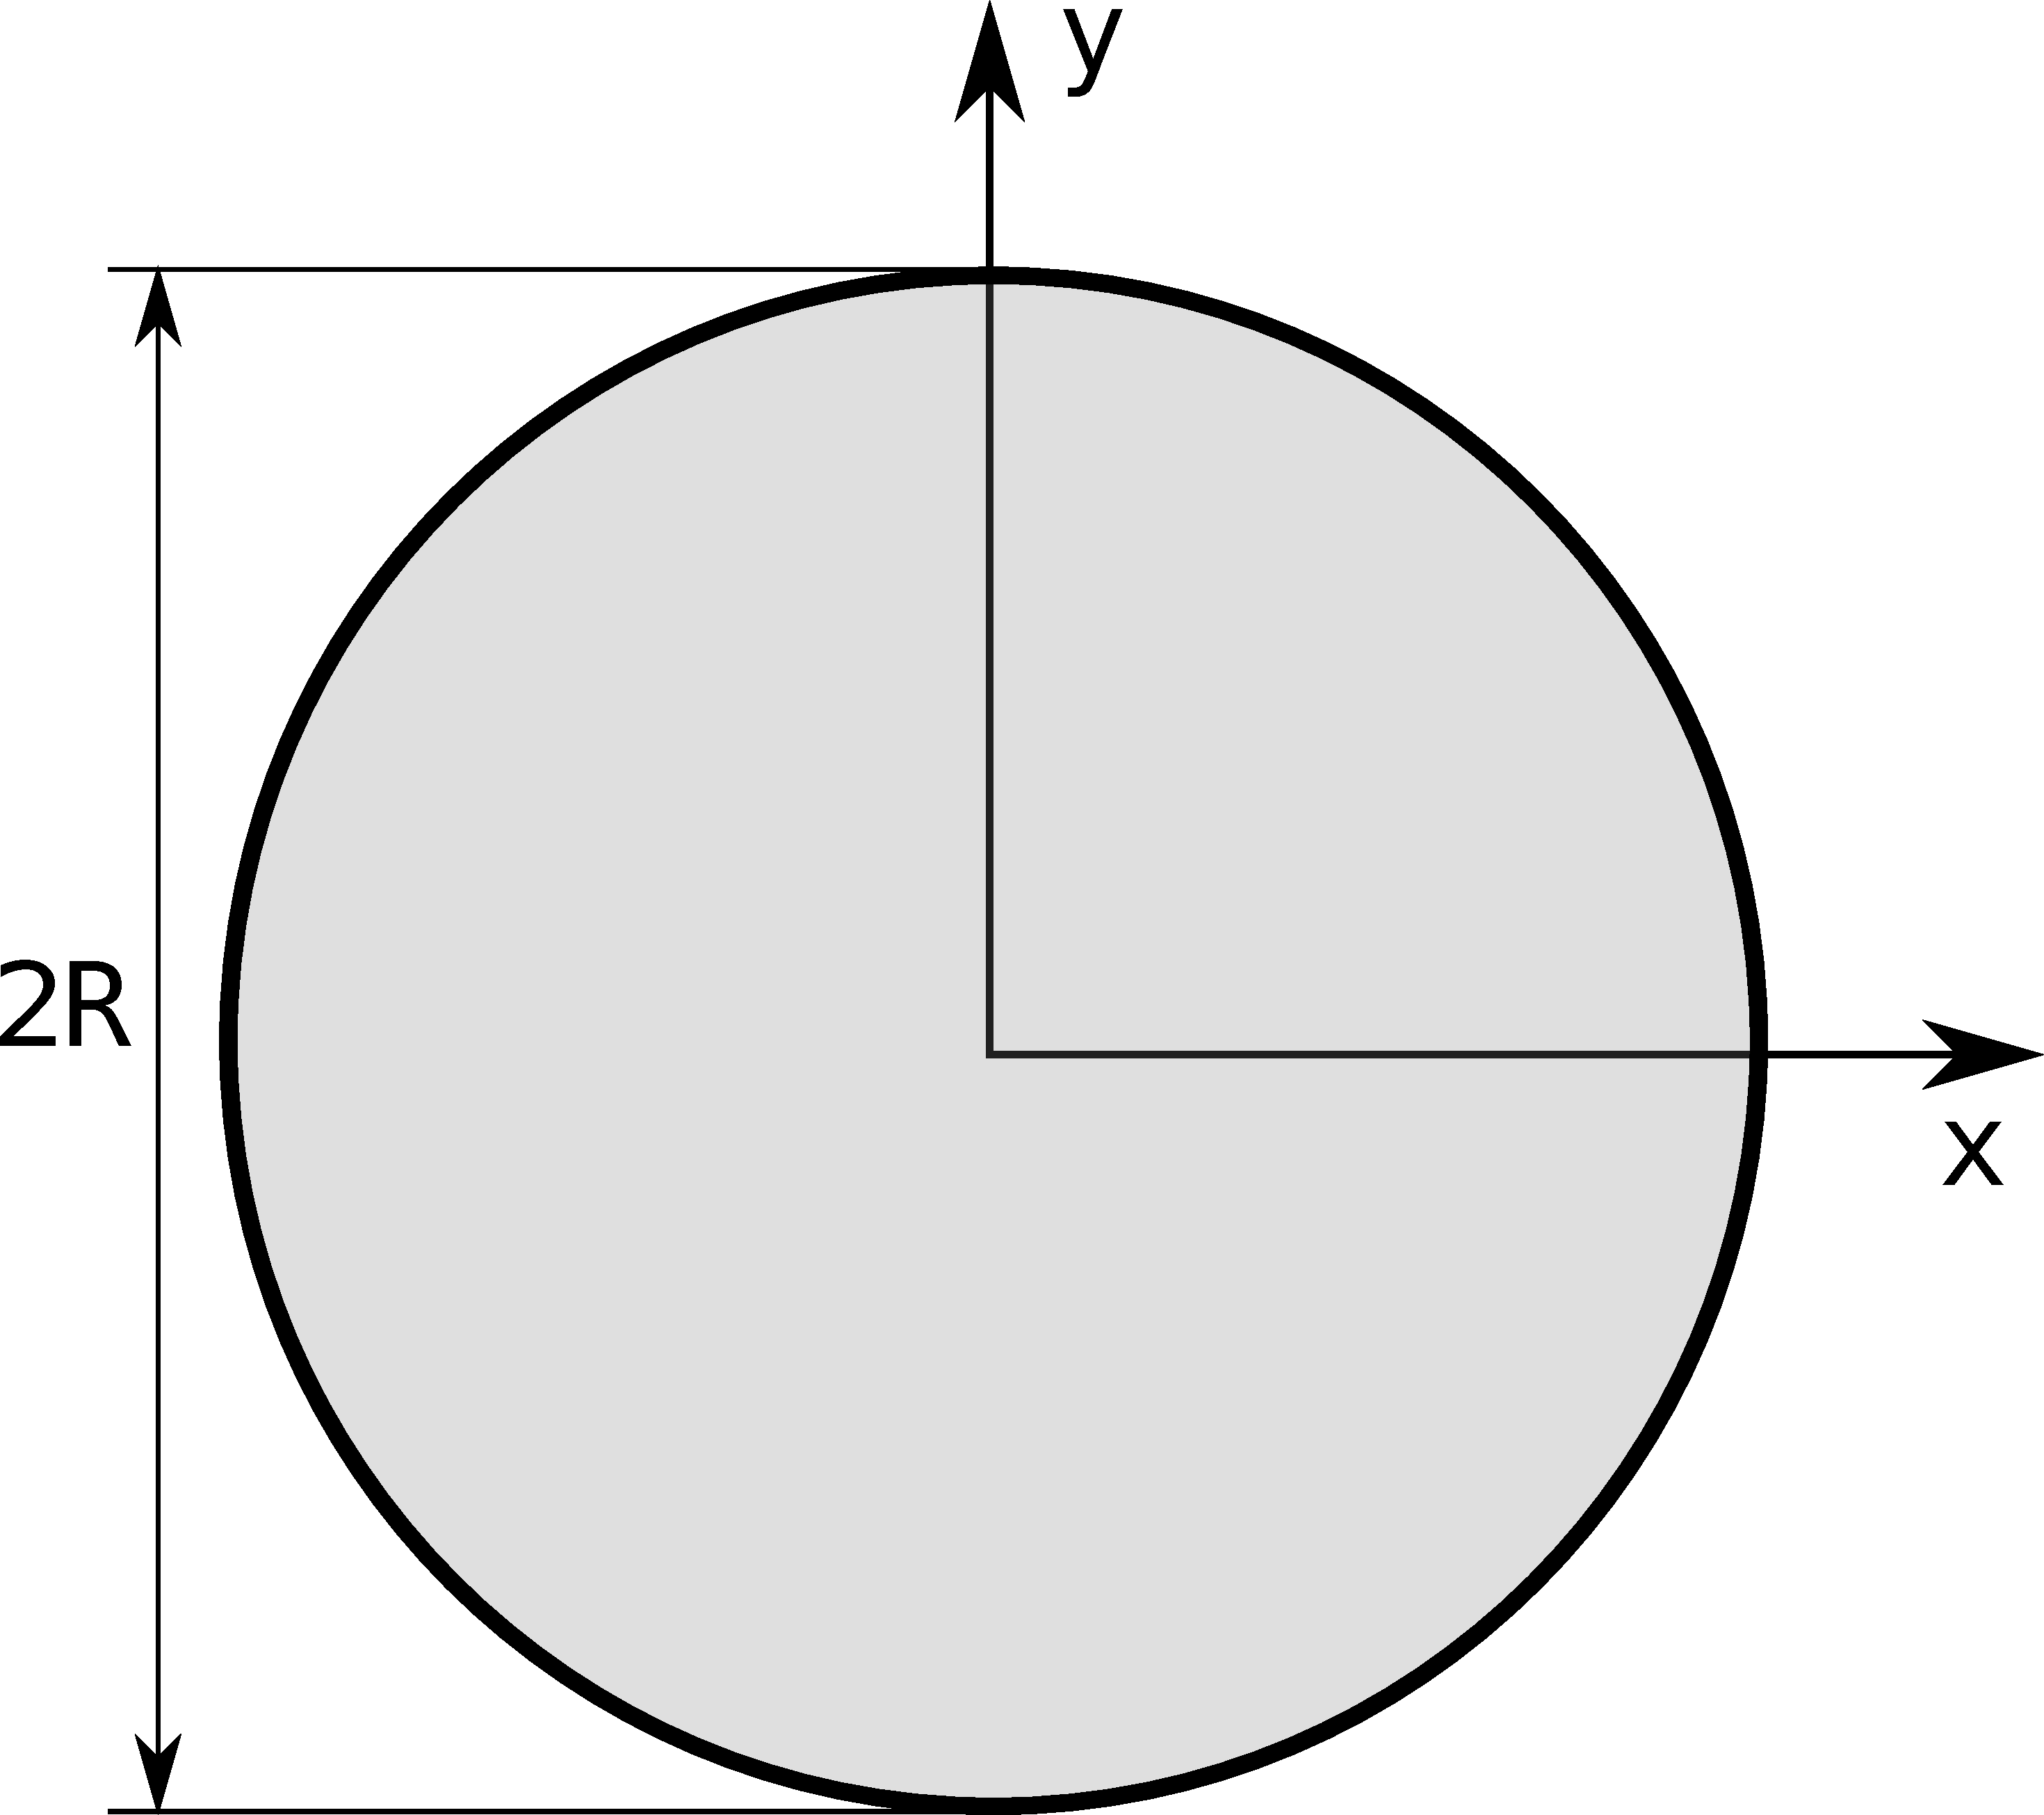
\includegraphics[width=.30\textwidth]{fig/cuts/FullSpheroid2dxy.pdf}}
\hfill
\subfigure[Side view]{\raisebox{-3mm}{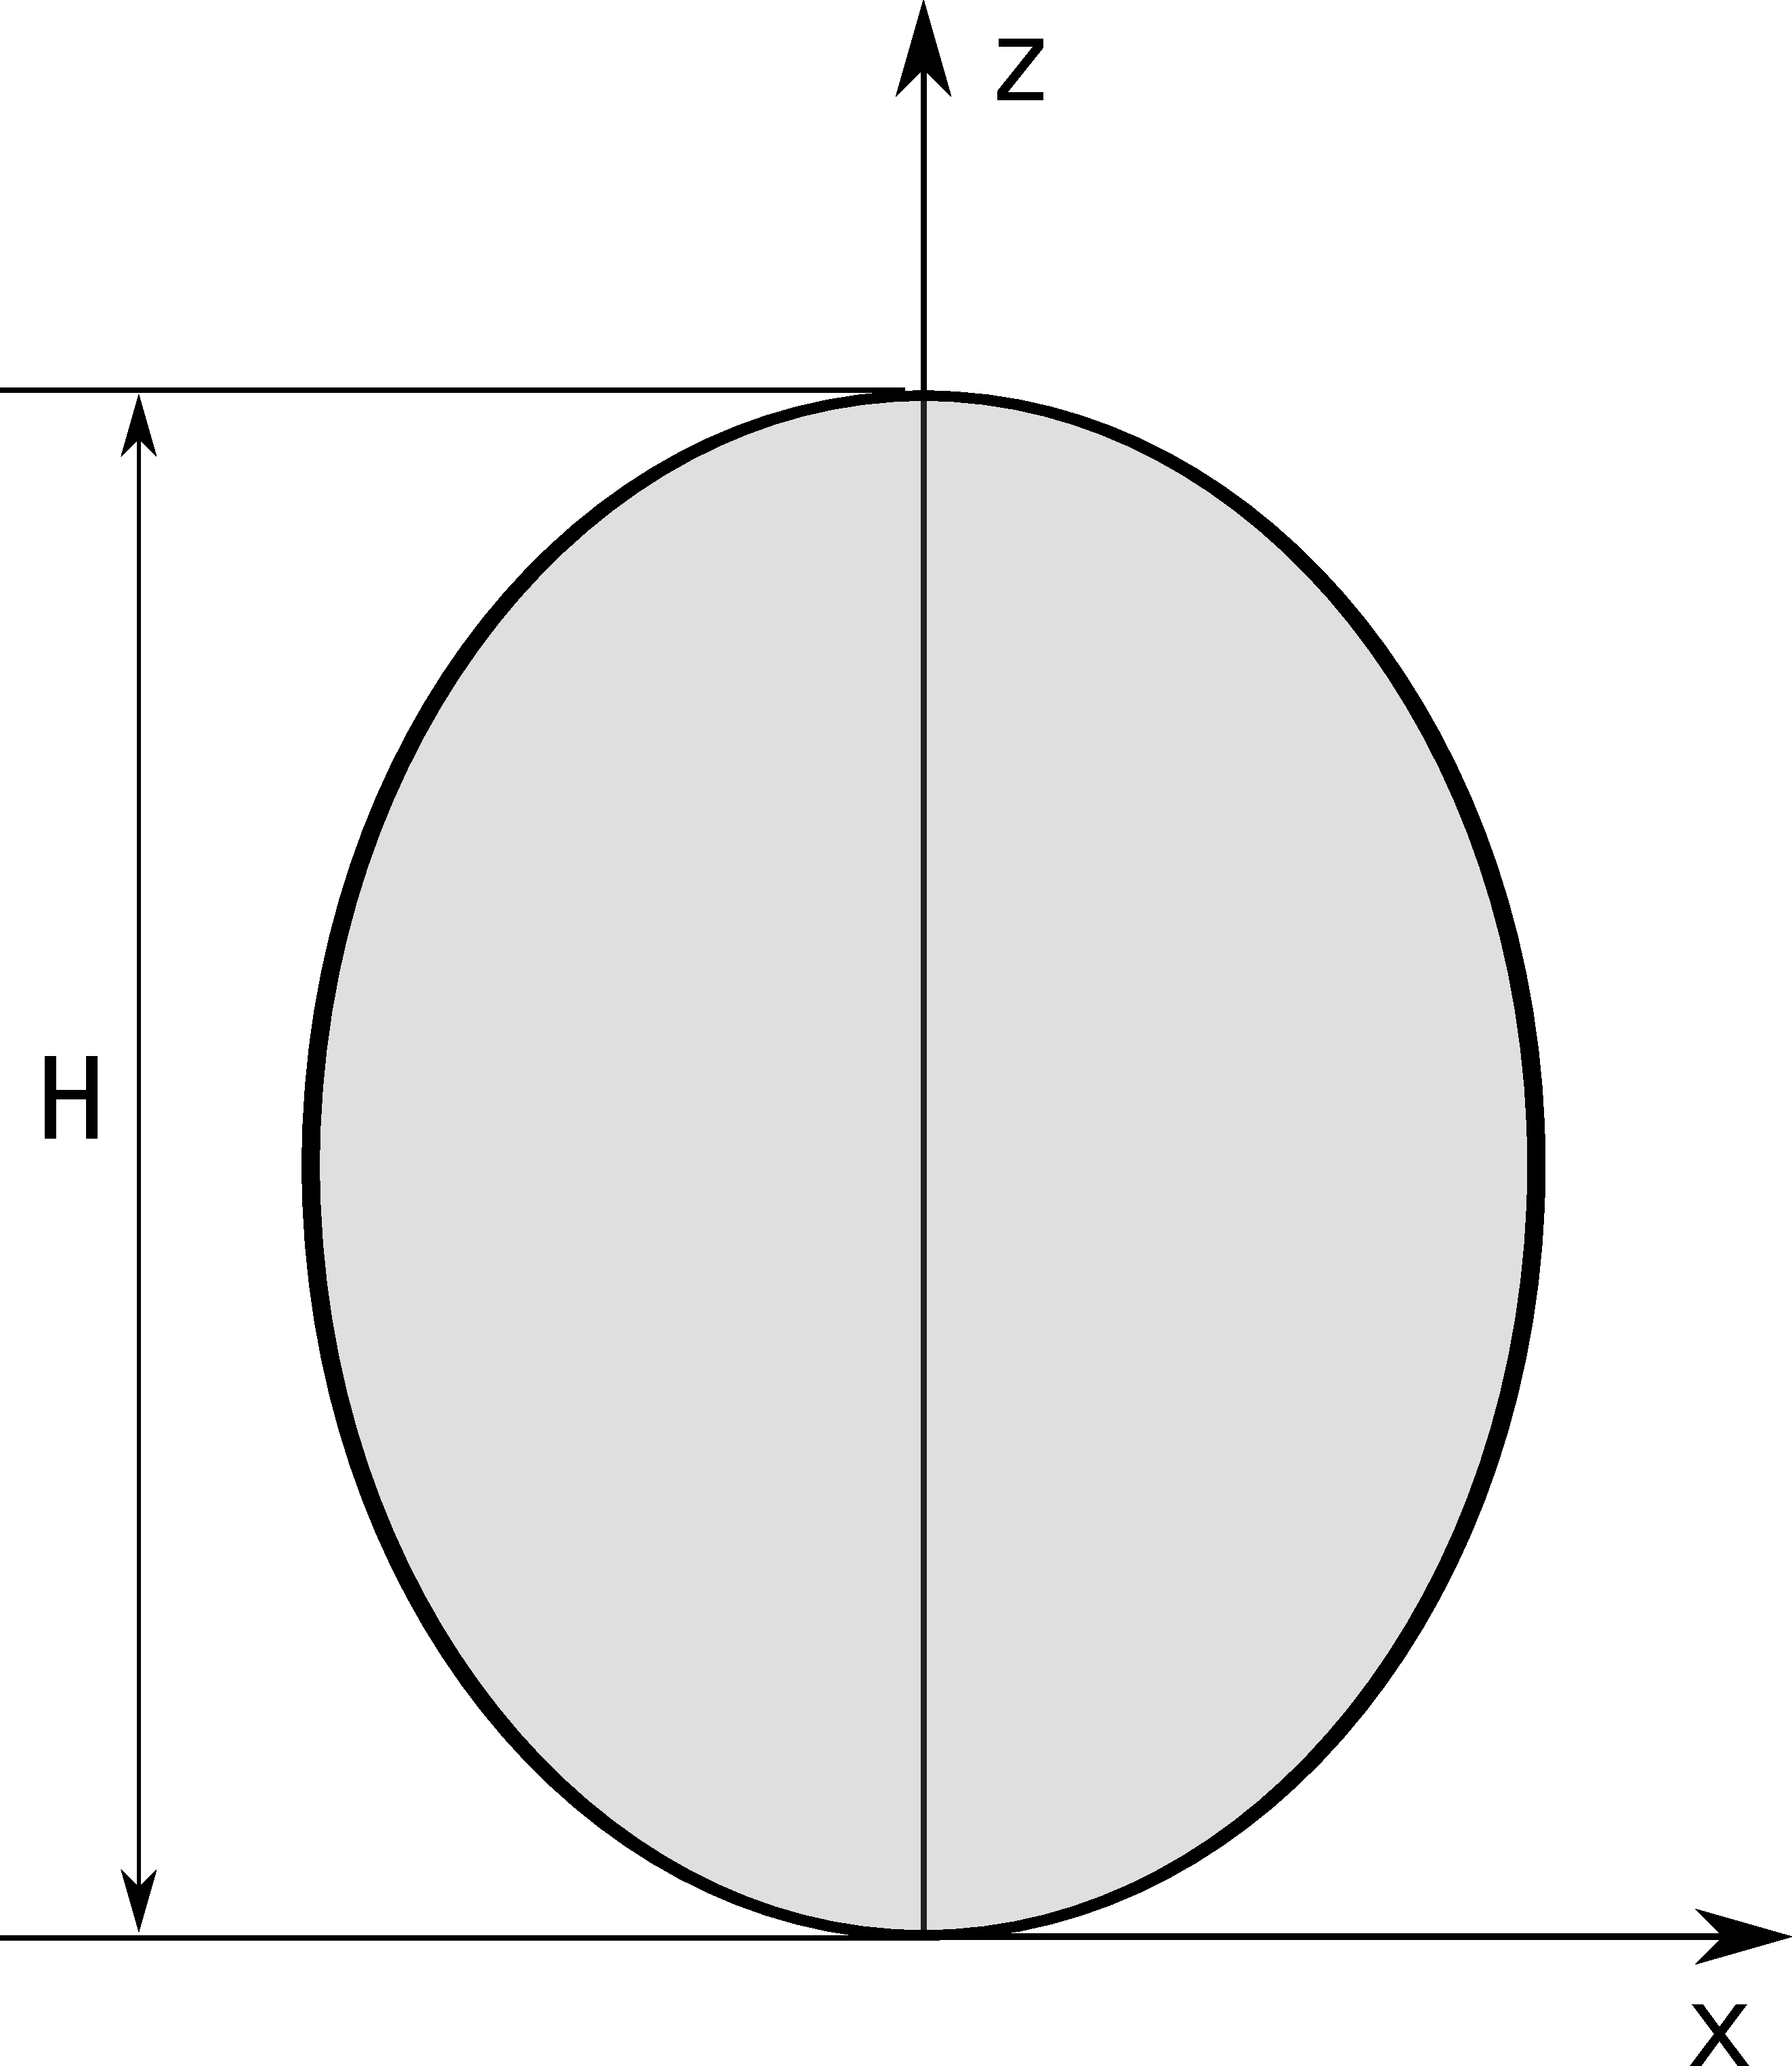
\includegraphics[width=.30\textwidth]{fig/cuts/FullSpheroid2dxz.pdf}}}
\hfill
\caption{A full spheroid, generated by rotating an ellipse around the vertical axis.}
\end{figure}

\FloatBarrier

\paragraph{Syntax and parameters}\strut\\[-2ex plus .2ex minus .2ex]
\begin{lstlisting}[language=python, style=eclipseboxed,numbers=none,nolol]
  FormFactorFullSpheroid(radius,height)
\end{lstlisting}
with the parameters
\begin{itemize}
\item \texttt{radius}, $R$,
\item \texttt{height}, $H$.
\end{itemize}


\paragraph{Form factor etc}\strut\\
Notation:
\begin{equation*}
 R_z \coloneqq R\sqrt{1-\frac{4z^2}{H^2}},\quad
 \gamma_z \coloneqq \sqrt{(q_x R_z)^2+(q_y R_z)^2}.  
\end{equation*}
Results:
\begin{equation*}
  F = 4\pi \exp(i q_z H/2) \int_0^{H/2} \!\d z\,
     R_z^2 \frac{J_1(q_{\parallel}R_z)}{q_{\parallel}R_z} \cos(q_z z),
\end{equation*}
\begin{equation*}
  V =\dfrac{2}{3}R^2H,
\end{equation*}
\begin{equation*}
  S =\pi R^2.
\end{equation*}

\paragraph{Example}\strut\\
Figure~\ref{fig:FFfspheroidEx} shows the normalized intensity
$|F|^2/V^2$, computed with $R=10$~nm, and $H=13$~nm.
\begin{figure}[H]
\begin{center}
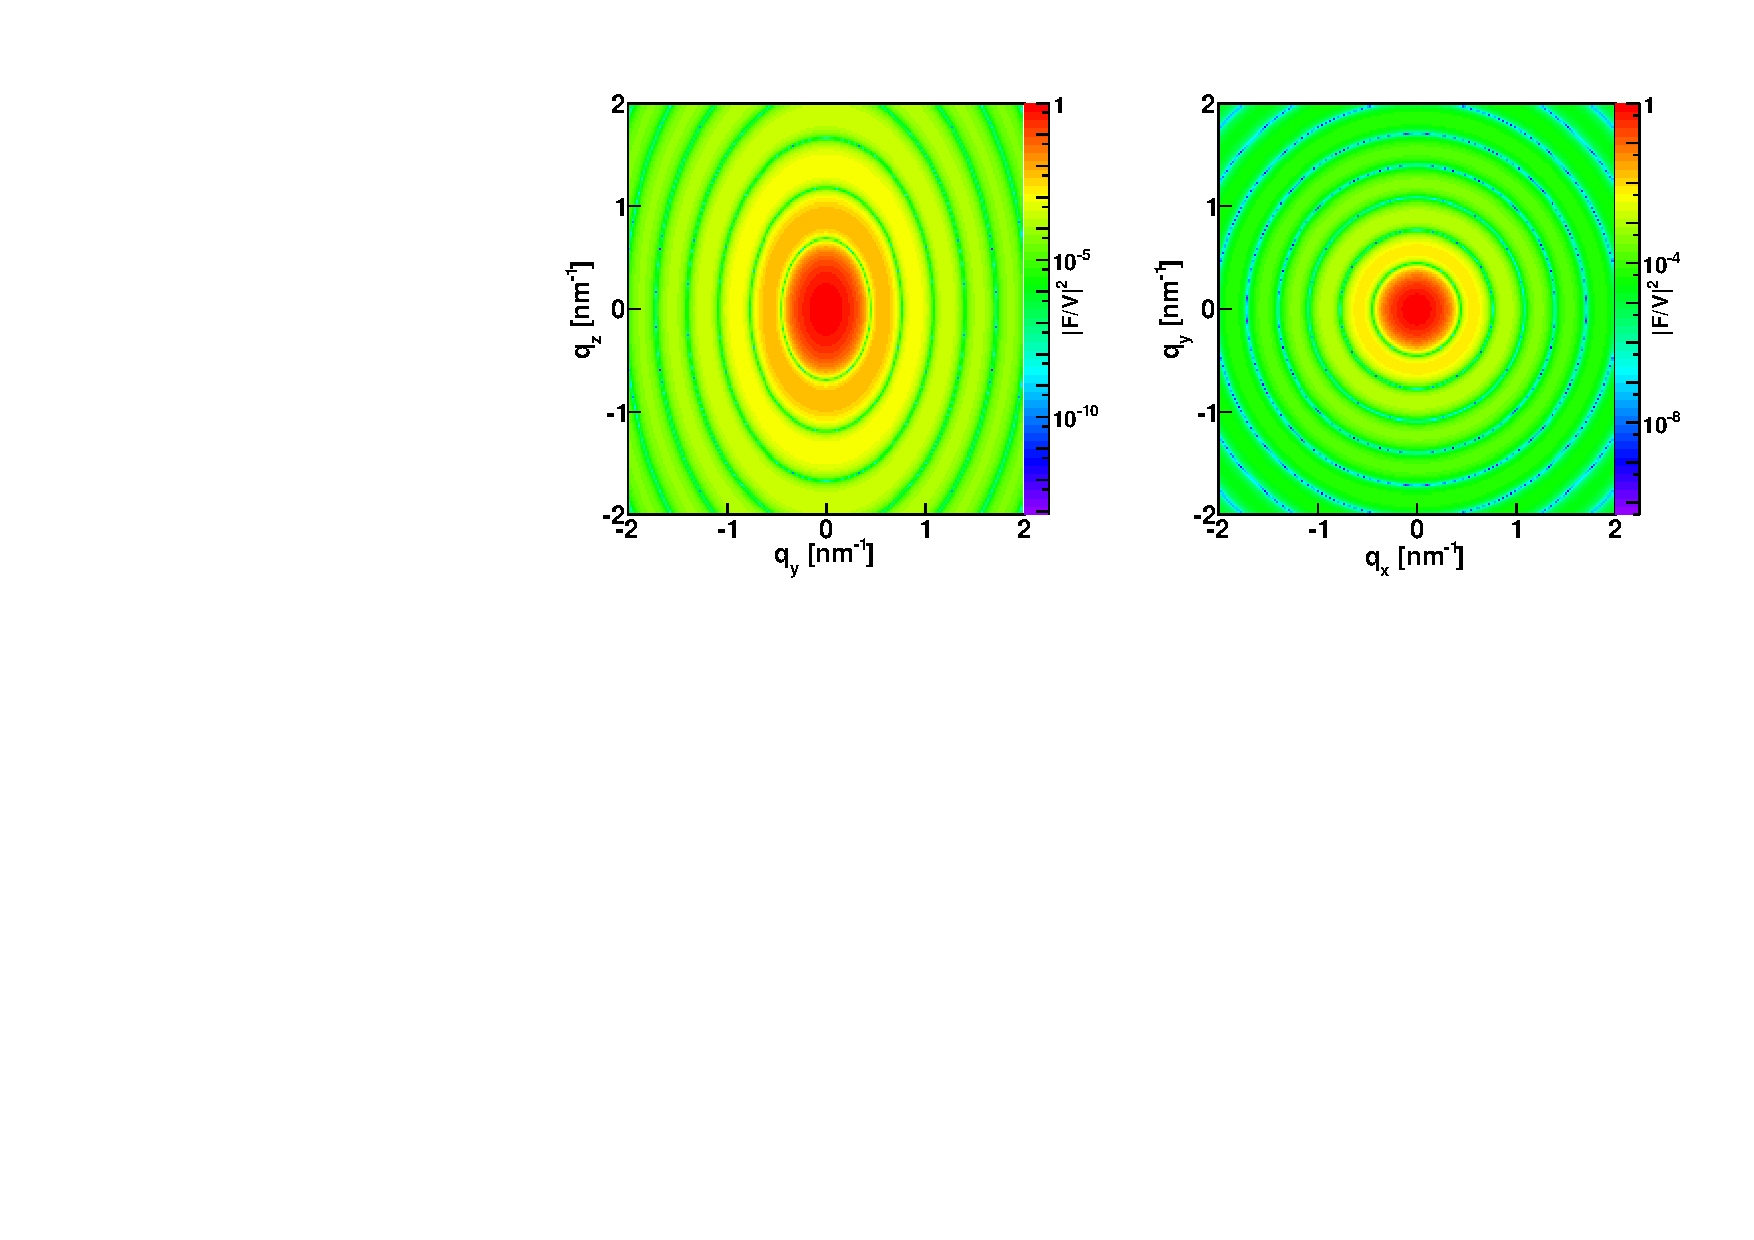
\includegraphics[angle=-90,width=\textwidth]{fig/ff/figfffspheroid.pdf}
\end{center}
\caption{Normalized intensity for the form factor of a full spheroid plotted against ($q_y$, $q_z$) and ($q_x$, $q_y$) and
  computed with \Code{FormFactorFullSpheroid(10.*nanometer, 13.*nanometer)}.}
\label{fig:FFfspheroidEx}
\end{figure}

\paragraph{References}\strut\\
Corrected version of the \lq\lq FullSpheroid\rq\rq\ form factor of \IsGISAXS~\cite{Laz02}.

%\subsection{References}
%The expression is identical to \Code{IsGISAXS} manual. In the code,
%the integration is over $[-H/2, H/2]$ with $\exp(iq_z z)$ instead of
%the cosine.
%In \Code{IsGISAXS}, factor 4 instead of 2 in the expression of the
%volume. In the code there is also a problem with an extra factor 2 in the function to integrate.


%-------------------------------------------------------------------------------
\clearpage
\subsection{Prism3 (triangular)} \label{sec:Prism3}
  \index{Prism (form factor)!triangular (Prism3)}
  \index{FormFactorPrism3@\Code{FormFactorPrism3}}
%-------------------------------------------------------------------------------

\paragraph{Real-space geometry}\strut\\

\begin{figure}[H]
\hfill
\subfigure[Perspective]{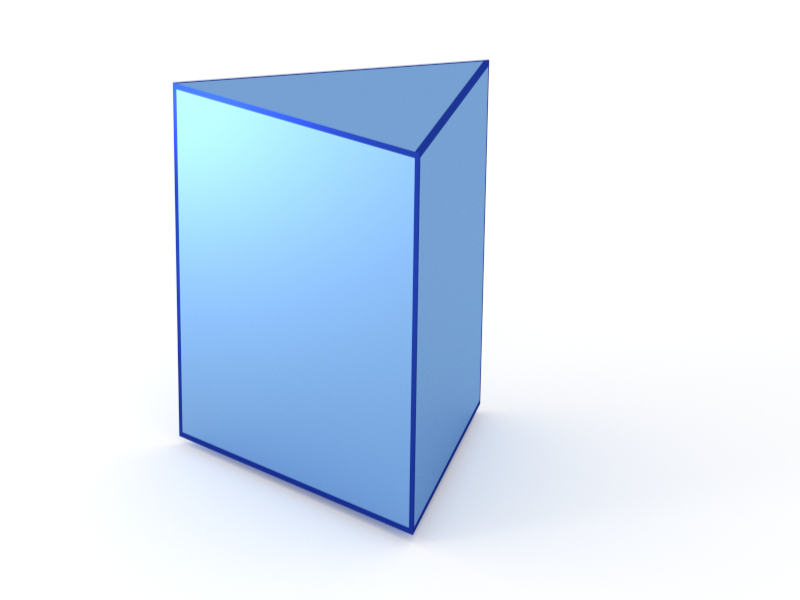
\includegraphics[width=.24\textwidth]{fig/blue/Prism33d.png}}
\hfill
\subfigure[Top view]{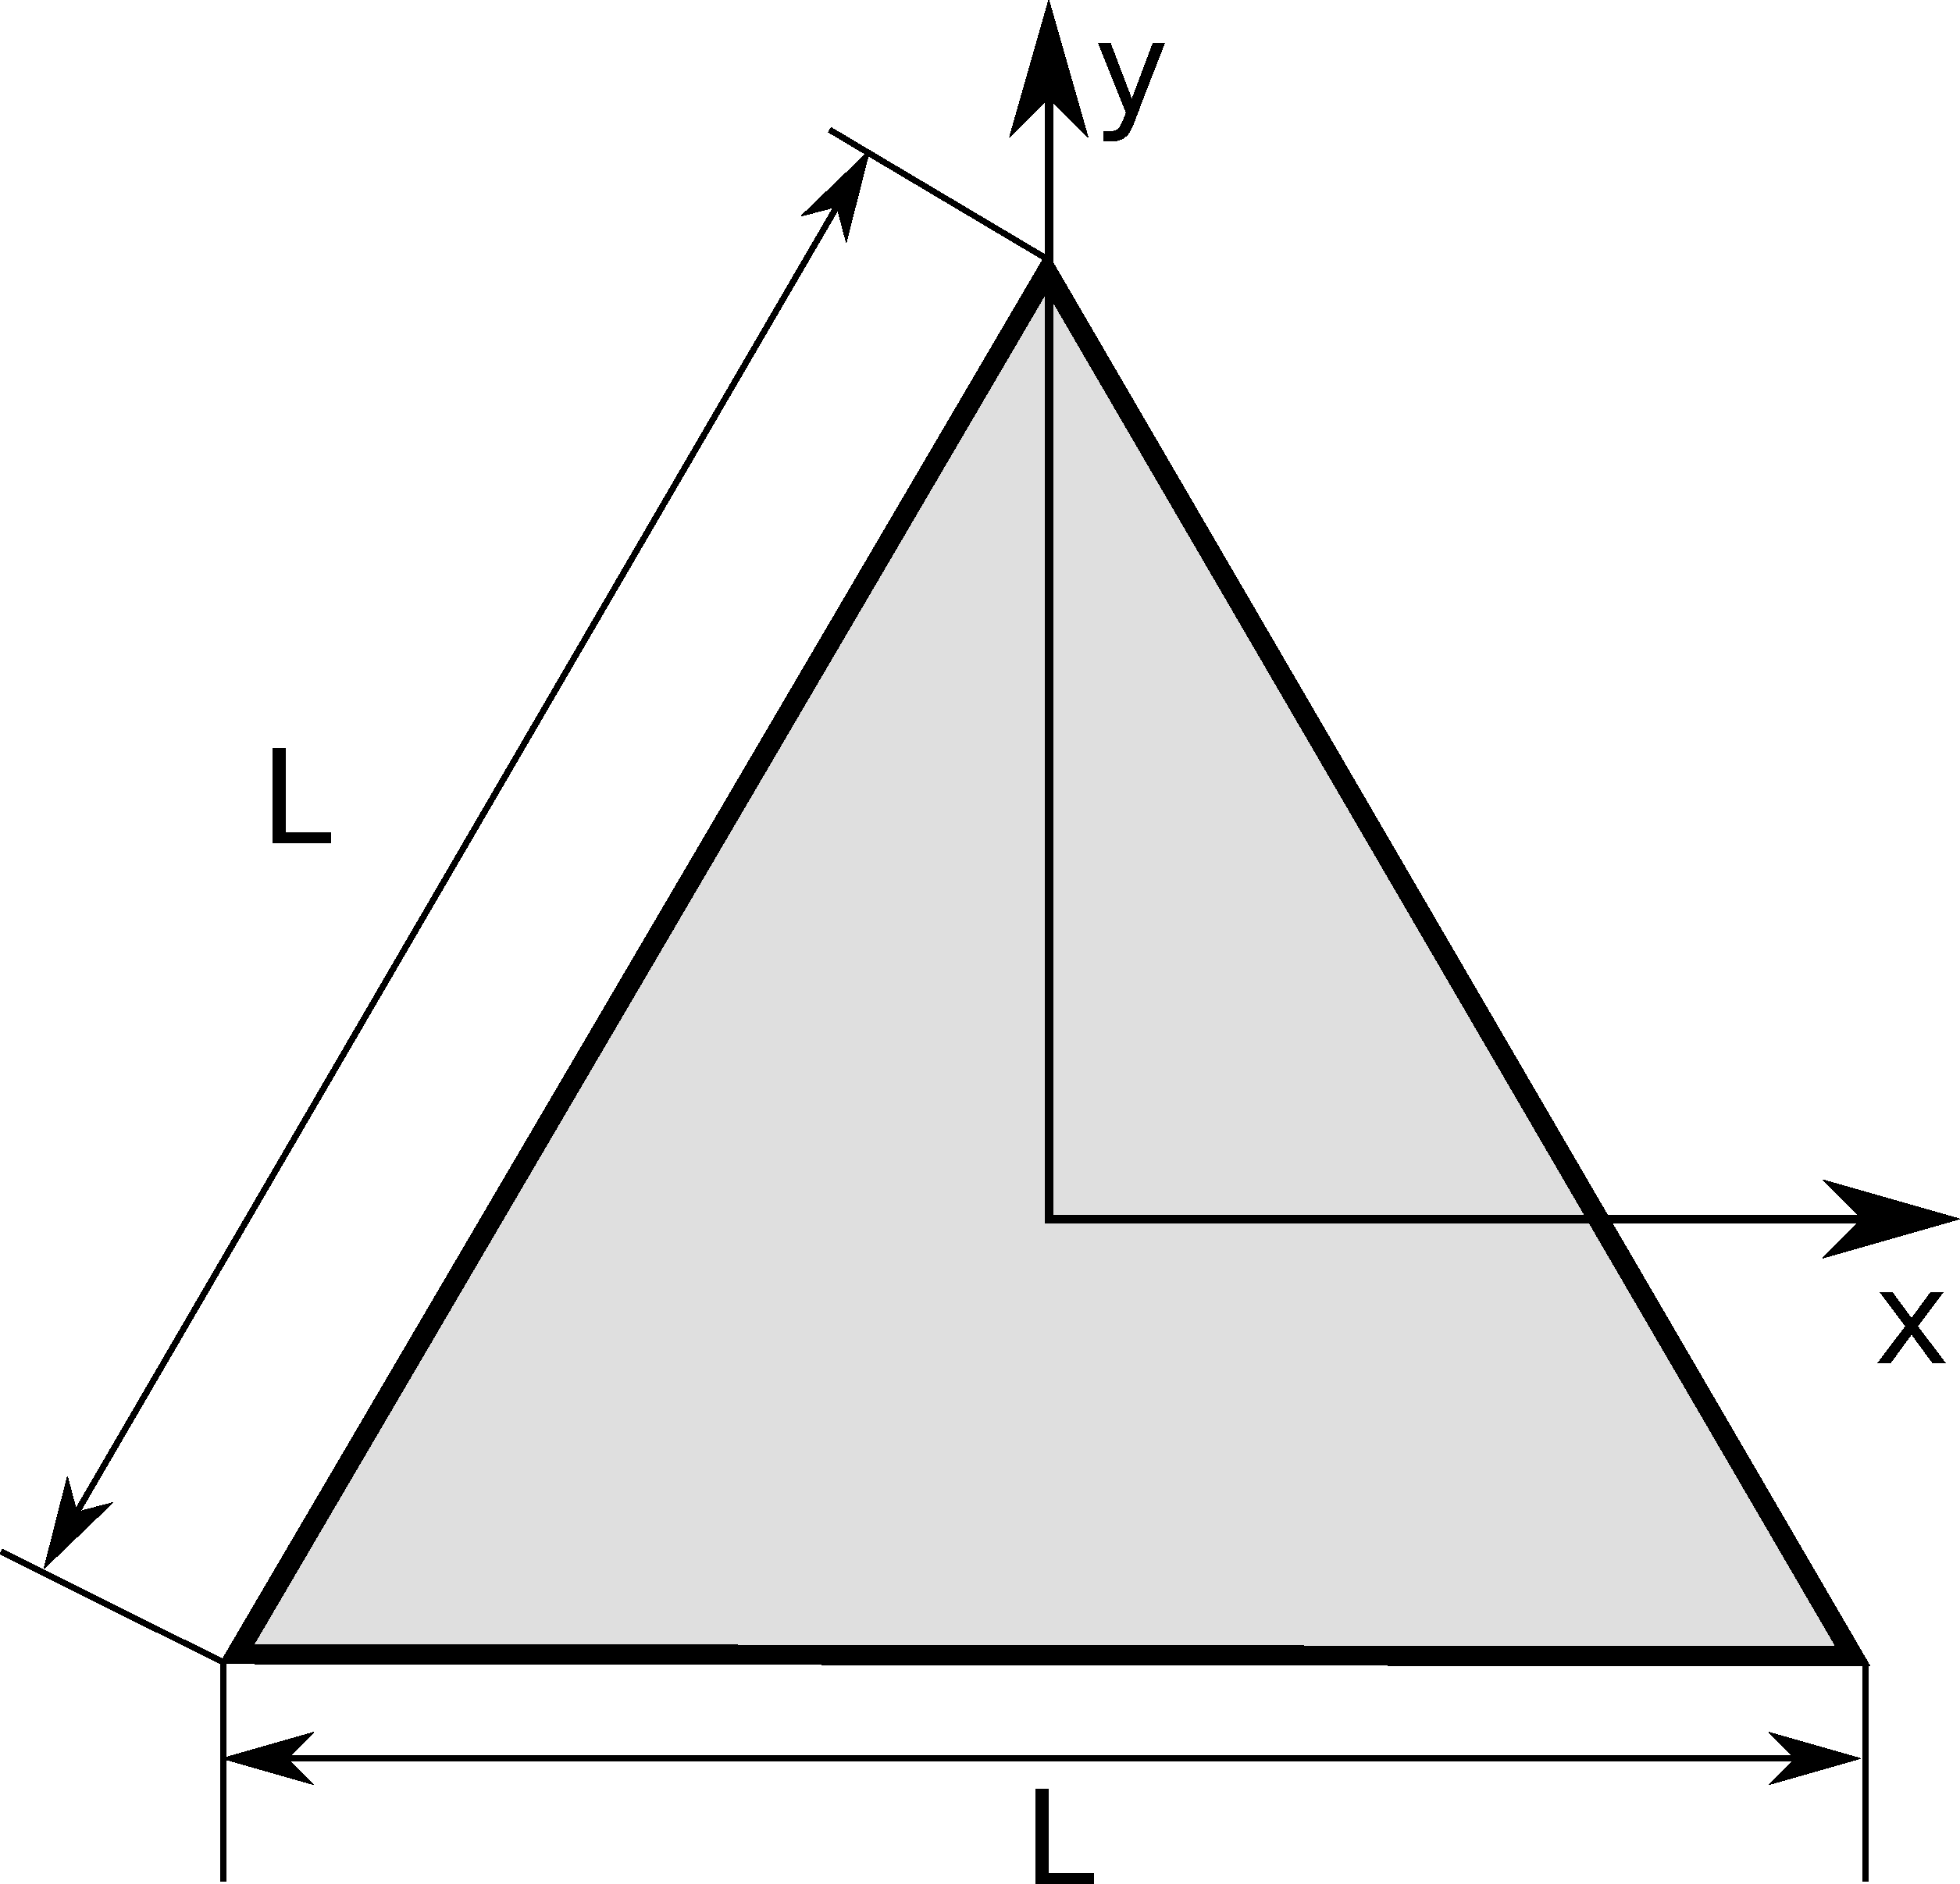
\includegraphics[width=.30\textwidth]{fig/cuts/Prism32dxy.pdf}}
\hfill
\subfigure[Side view]{\raisebox{2mm}{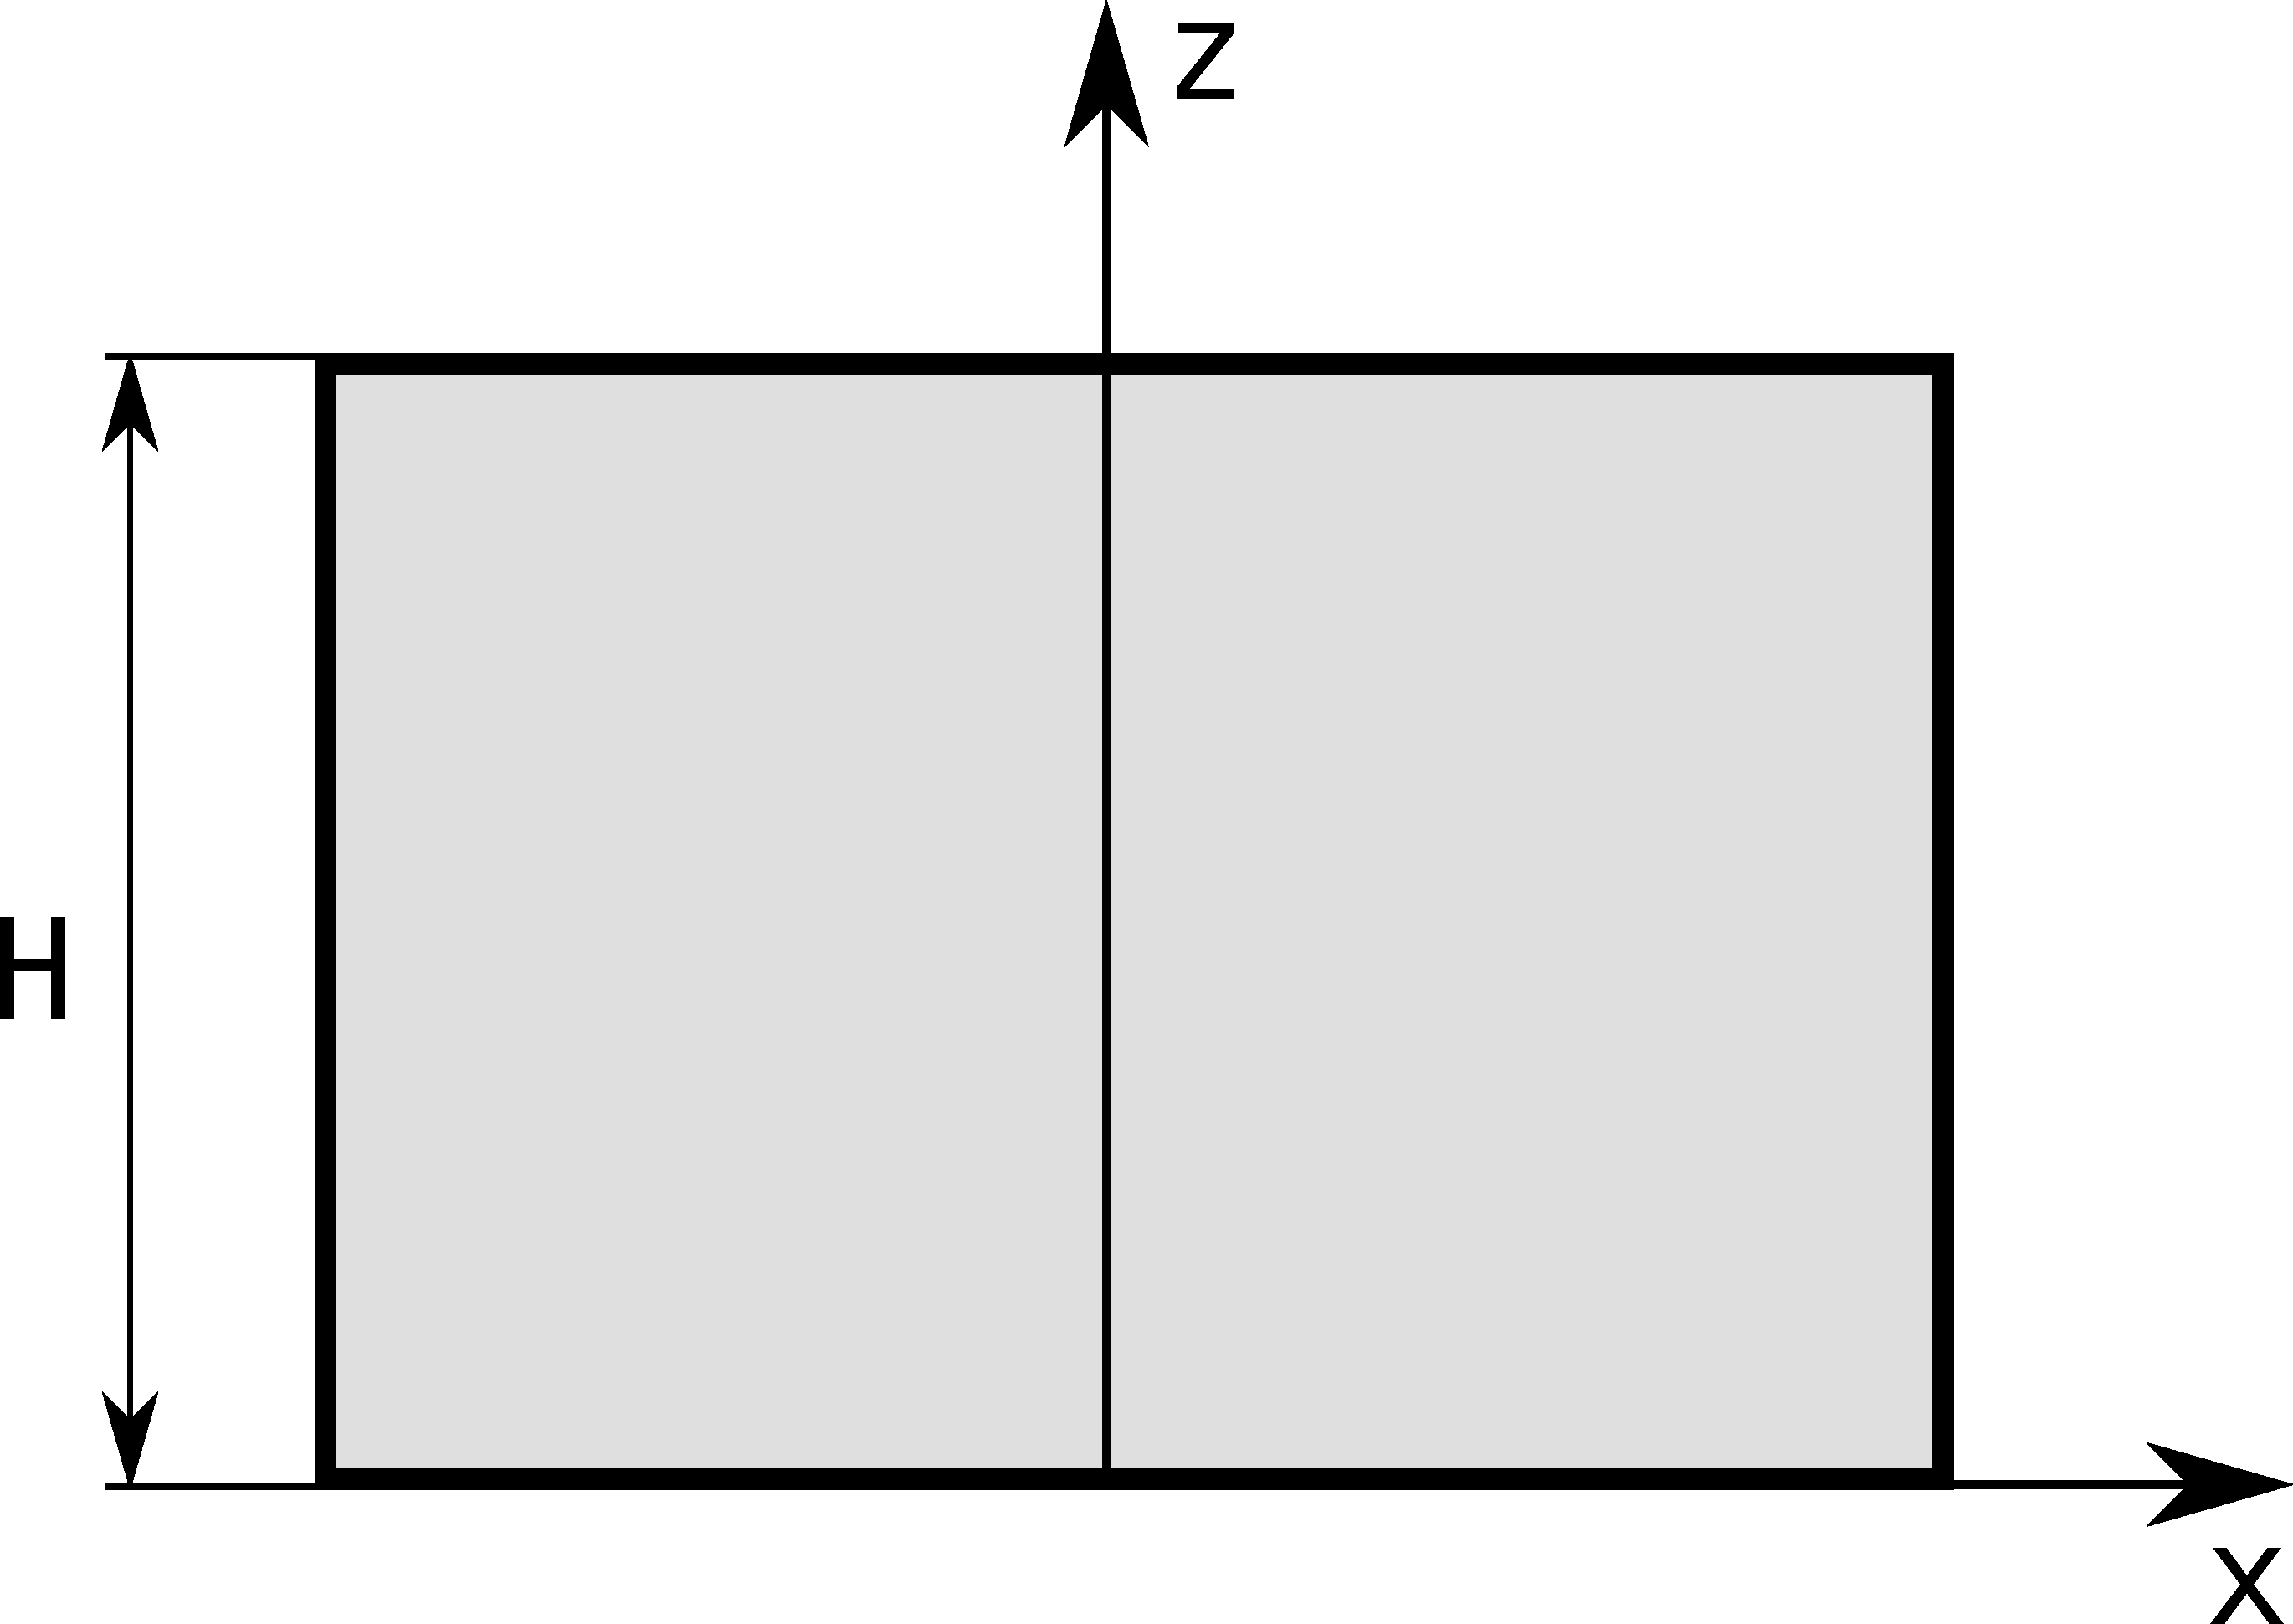
\includegraphics[width=.30\textwidth]{fig/cuts/Prism32dxz.pdf}}}
\hfill
\caption{A prism based on an equilateral triangle.}
\end{figure}

\FloatBarrier

\paragraph{Syntax and parameters}\strut\\[-2ex plus .2ex minus .2ex]
\begin{lstlisting}[language=python, style=eclipseboxed,numbers=none,nolol]
  FormFactorPrism3(length, height)
\end{lstlisting}
with the parameters
\begin{itemize}
\item \texttt{length} of one base edge, $L$,
\item \texttt{height}, $H$.
\end{itemize}


\paragraph{Form factor etc}\strut\\
\begin{align*}
F &= \frac{2 \sqrt{3}}{q_x^2-3q_y^2} 
     \exp\left(-i q_y\frac{L}{2\sqrt{3}}\right)
    \left[\exp\left(i \sqrt{3} q_y \frac{L}{2} \right)-\cos\left(q_x \frac{L}{2}\right)
    -i \sqrt{3} q_y \frac{L}{2} \sinc\left(q_x \frac{L}{2}\right) \right] \\
  &
  \times  H \sinc\left(q_z \frac{H}{2} \right) \exp\left(i q_z \frac{H}{2}\right),
\end{align*}
\begin{equation*}
  V= \dfrac{\sqrt{3}}{4} H L^2,
\end{equation*}
\begin{equation*}
  S =\dfrac{\sqrt{3}}{4}L^2.
\end{equation*}

\paragraph{Example}\strut\\
Figure~\ref{fig:FFprism3Ex} shows the normalized intensity
$|F|^2/V^2$, computed with $L=10$~nm and \mbox{$H=13$~nm.}
\begin{figure}[H]
\begin{center}
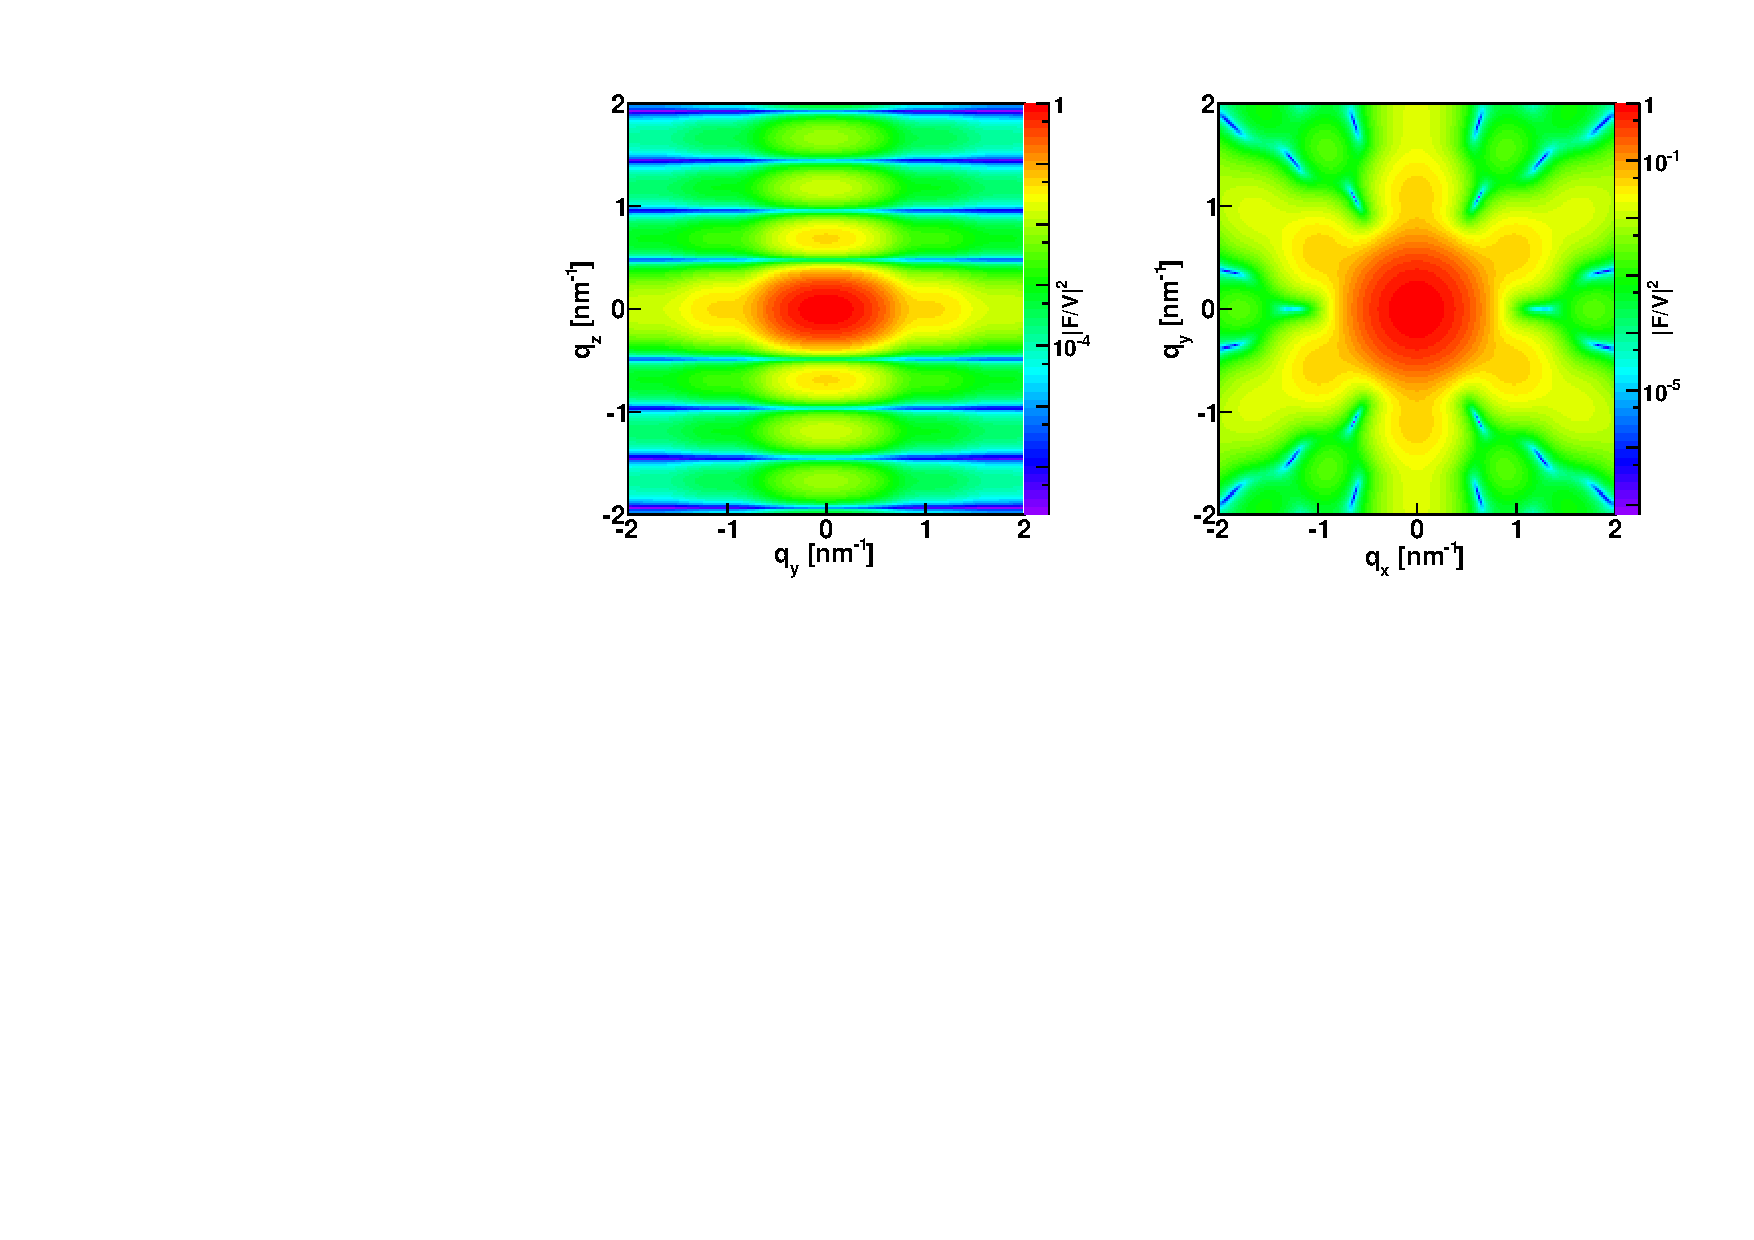
\includegraphics[angle=-90,width=\textwidth]{fig/ff/figffprism3.pdf}
\end{center}
\caption{Normalized intensity for the form factor of a Prism3
 plotted against ($q_y$, $q_z$) and  ($q_x$, $q_y$) and
  computed with \Code{FormFactorPrism3(10.*nanometer, 13.*nanometer)}.}
\label{fig:FFprism3Ex}
\end{figure}

\paragraph{References}\strut\\
Agrees with \E{Prism3} form factor of \IsGISAXS\
\cite[Eq.~2.29]{Laz08} \cite[Eq.~219]{ReLL09},
except for the definition of parameter $L= 2 R_{\rm{\Code{IsGISAXS}}}$.

%-------------------------------------------------------------------------------
\clearpage
\subsection{Prism6 (hexagonal)} \label{sec:Prism6}
  \index{Prism (form factor)!hexagonal (Prism6)}
  \index{FormFactorPrism6@\Code{FormFactorPrism6}}
%-------------------------------------------------------------------------------

\paragraph{Real-space geometry}\strut\\

\begin{figure}[H]
\hfill
\subfigure[Perspective]{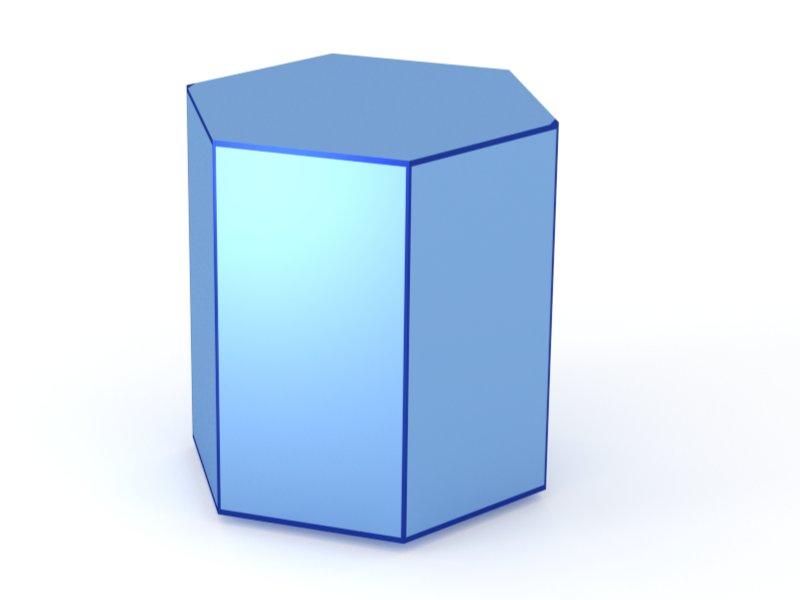
\includegraphics[width=.24\textwidth]{fig/blue/Prism63d.png}}
\hfill
\subfigure[Top view]{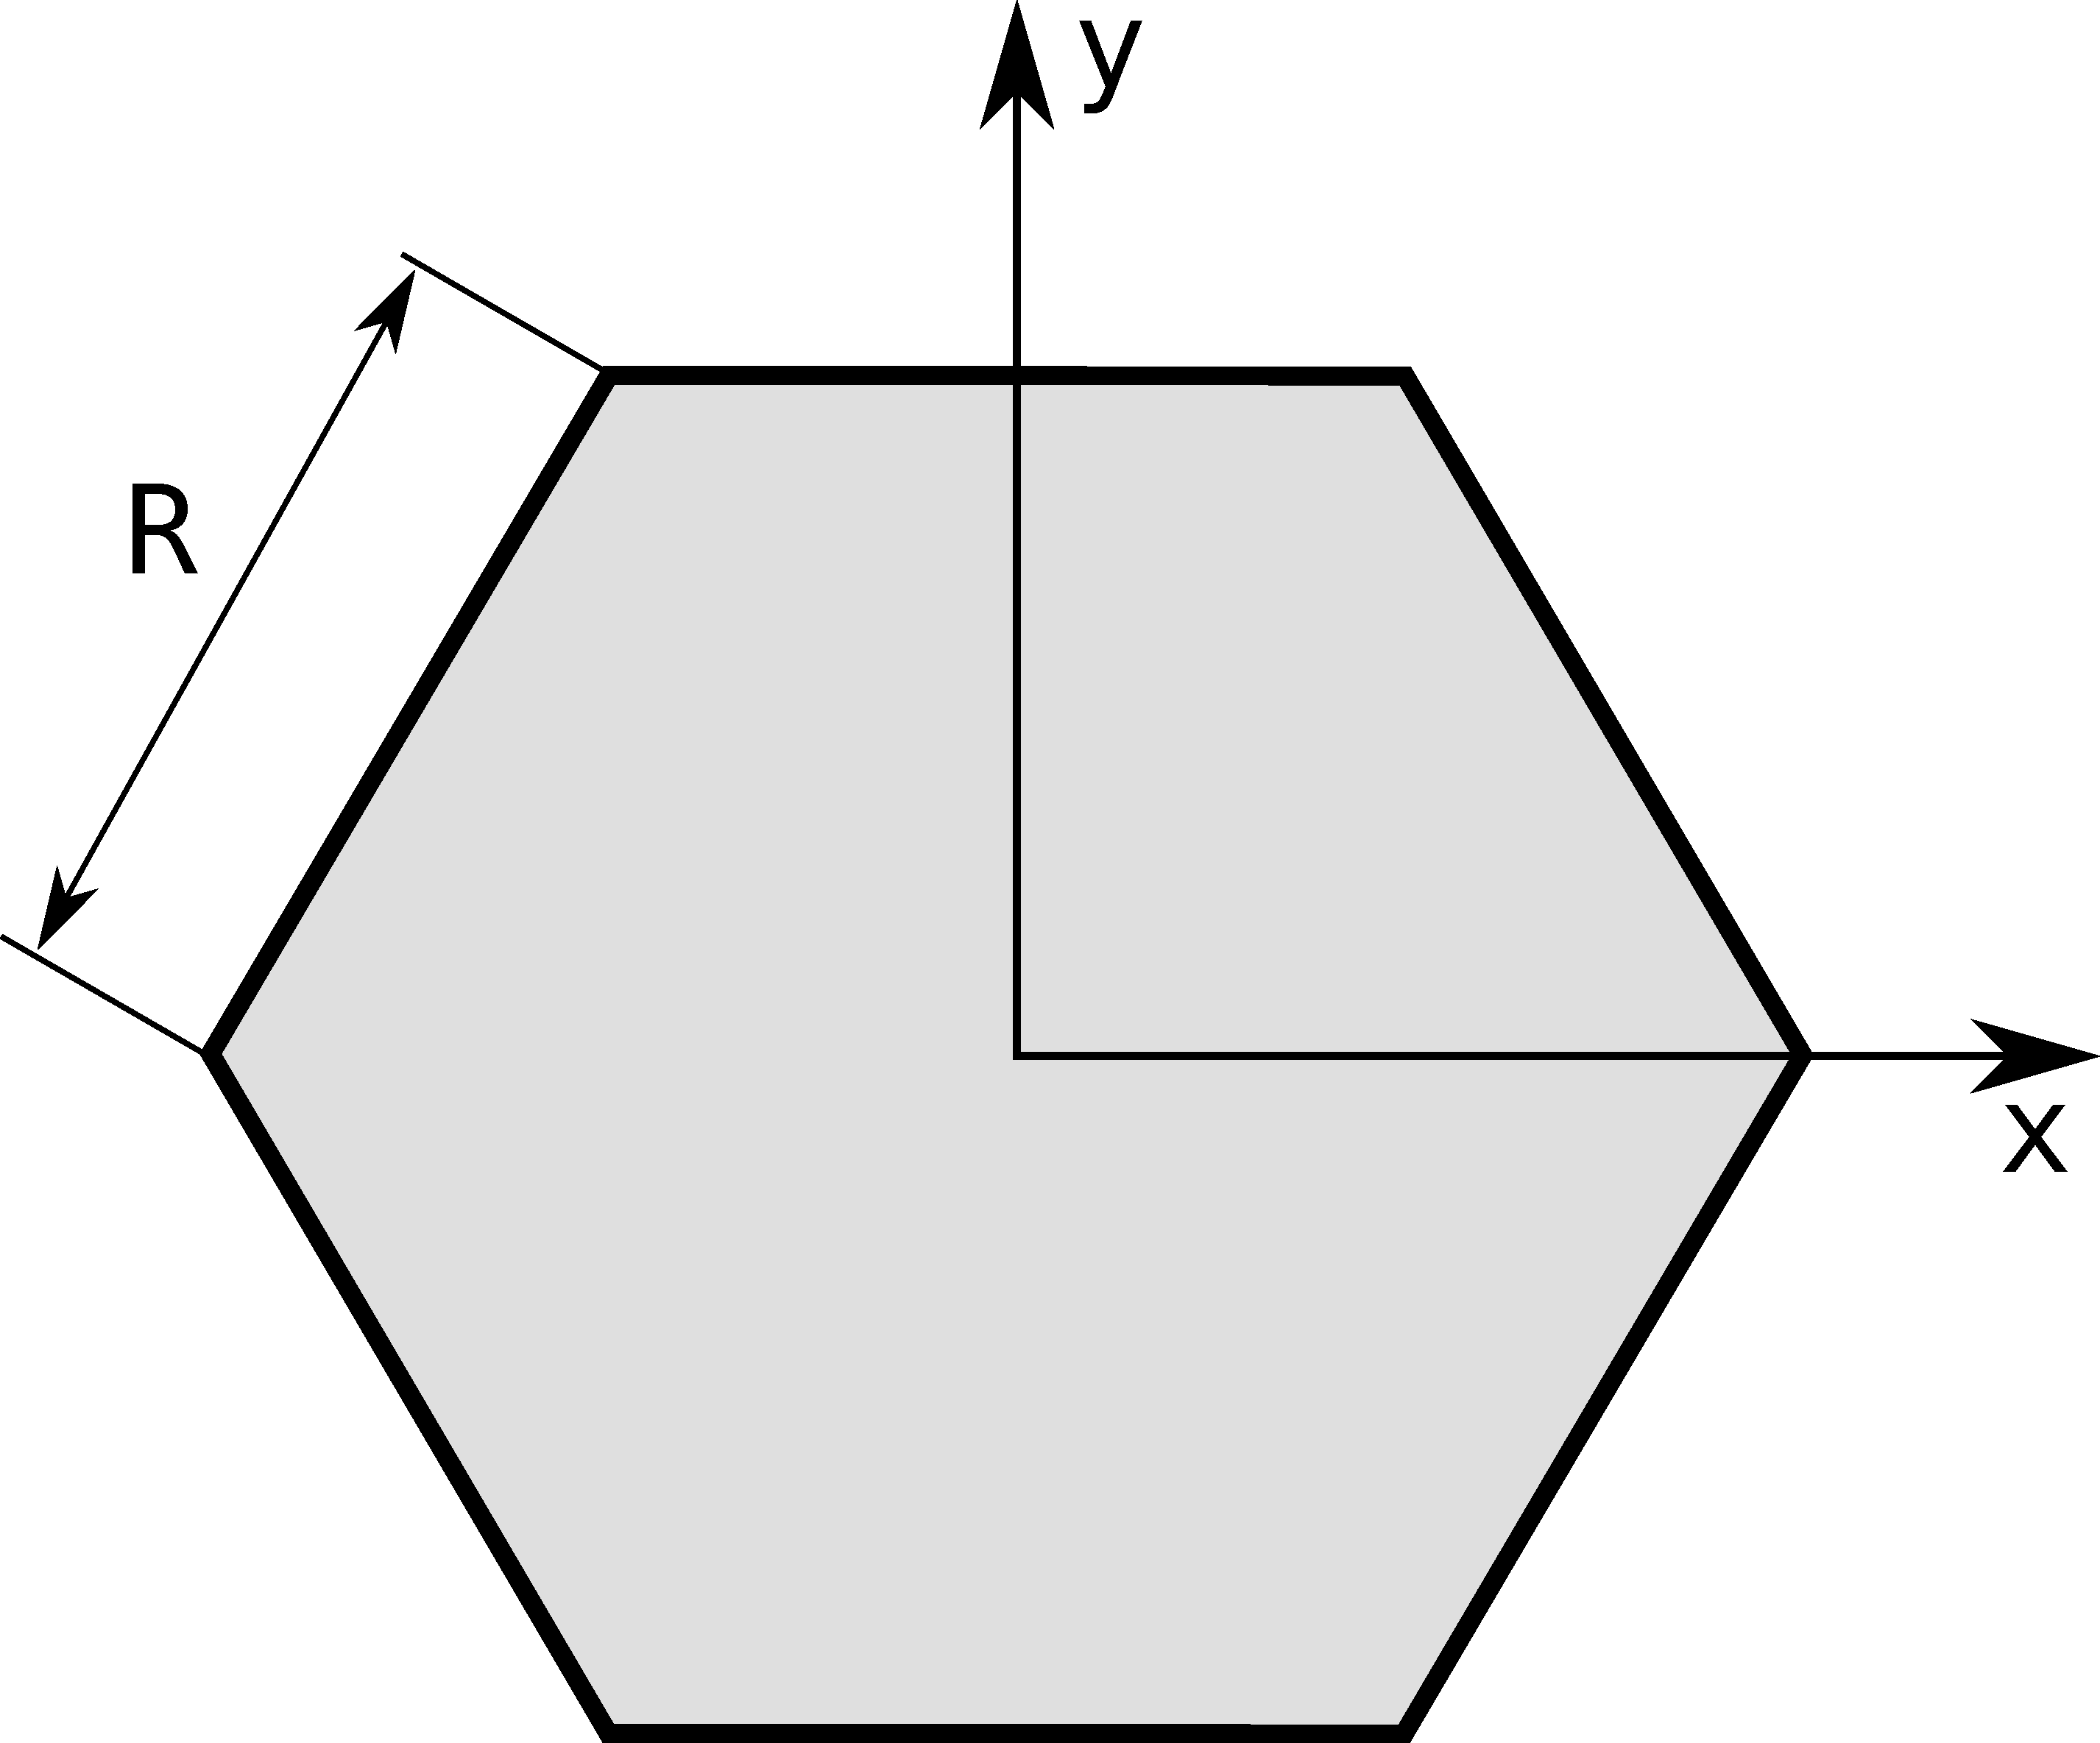
\includegraphics[width=.30\textwidth]{fig/cuts/Prism62dxy.pdf}}
\hfill
\subfigure[Side view]{\raisebox{-3mm}{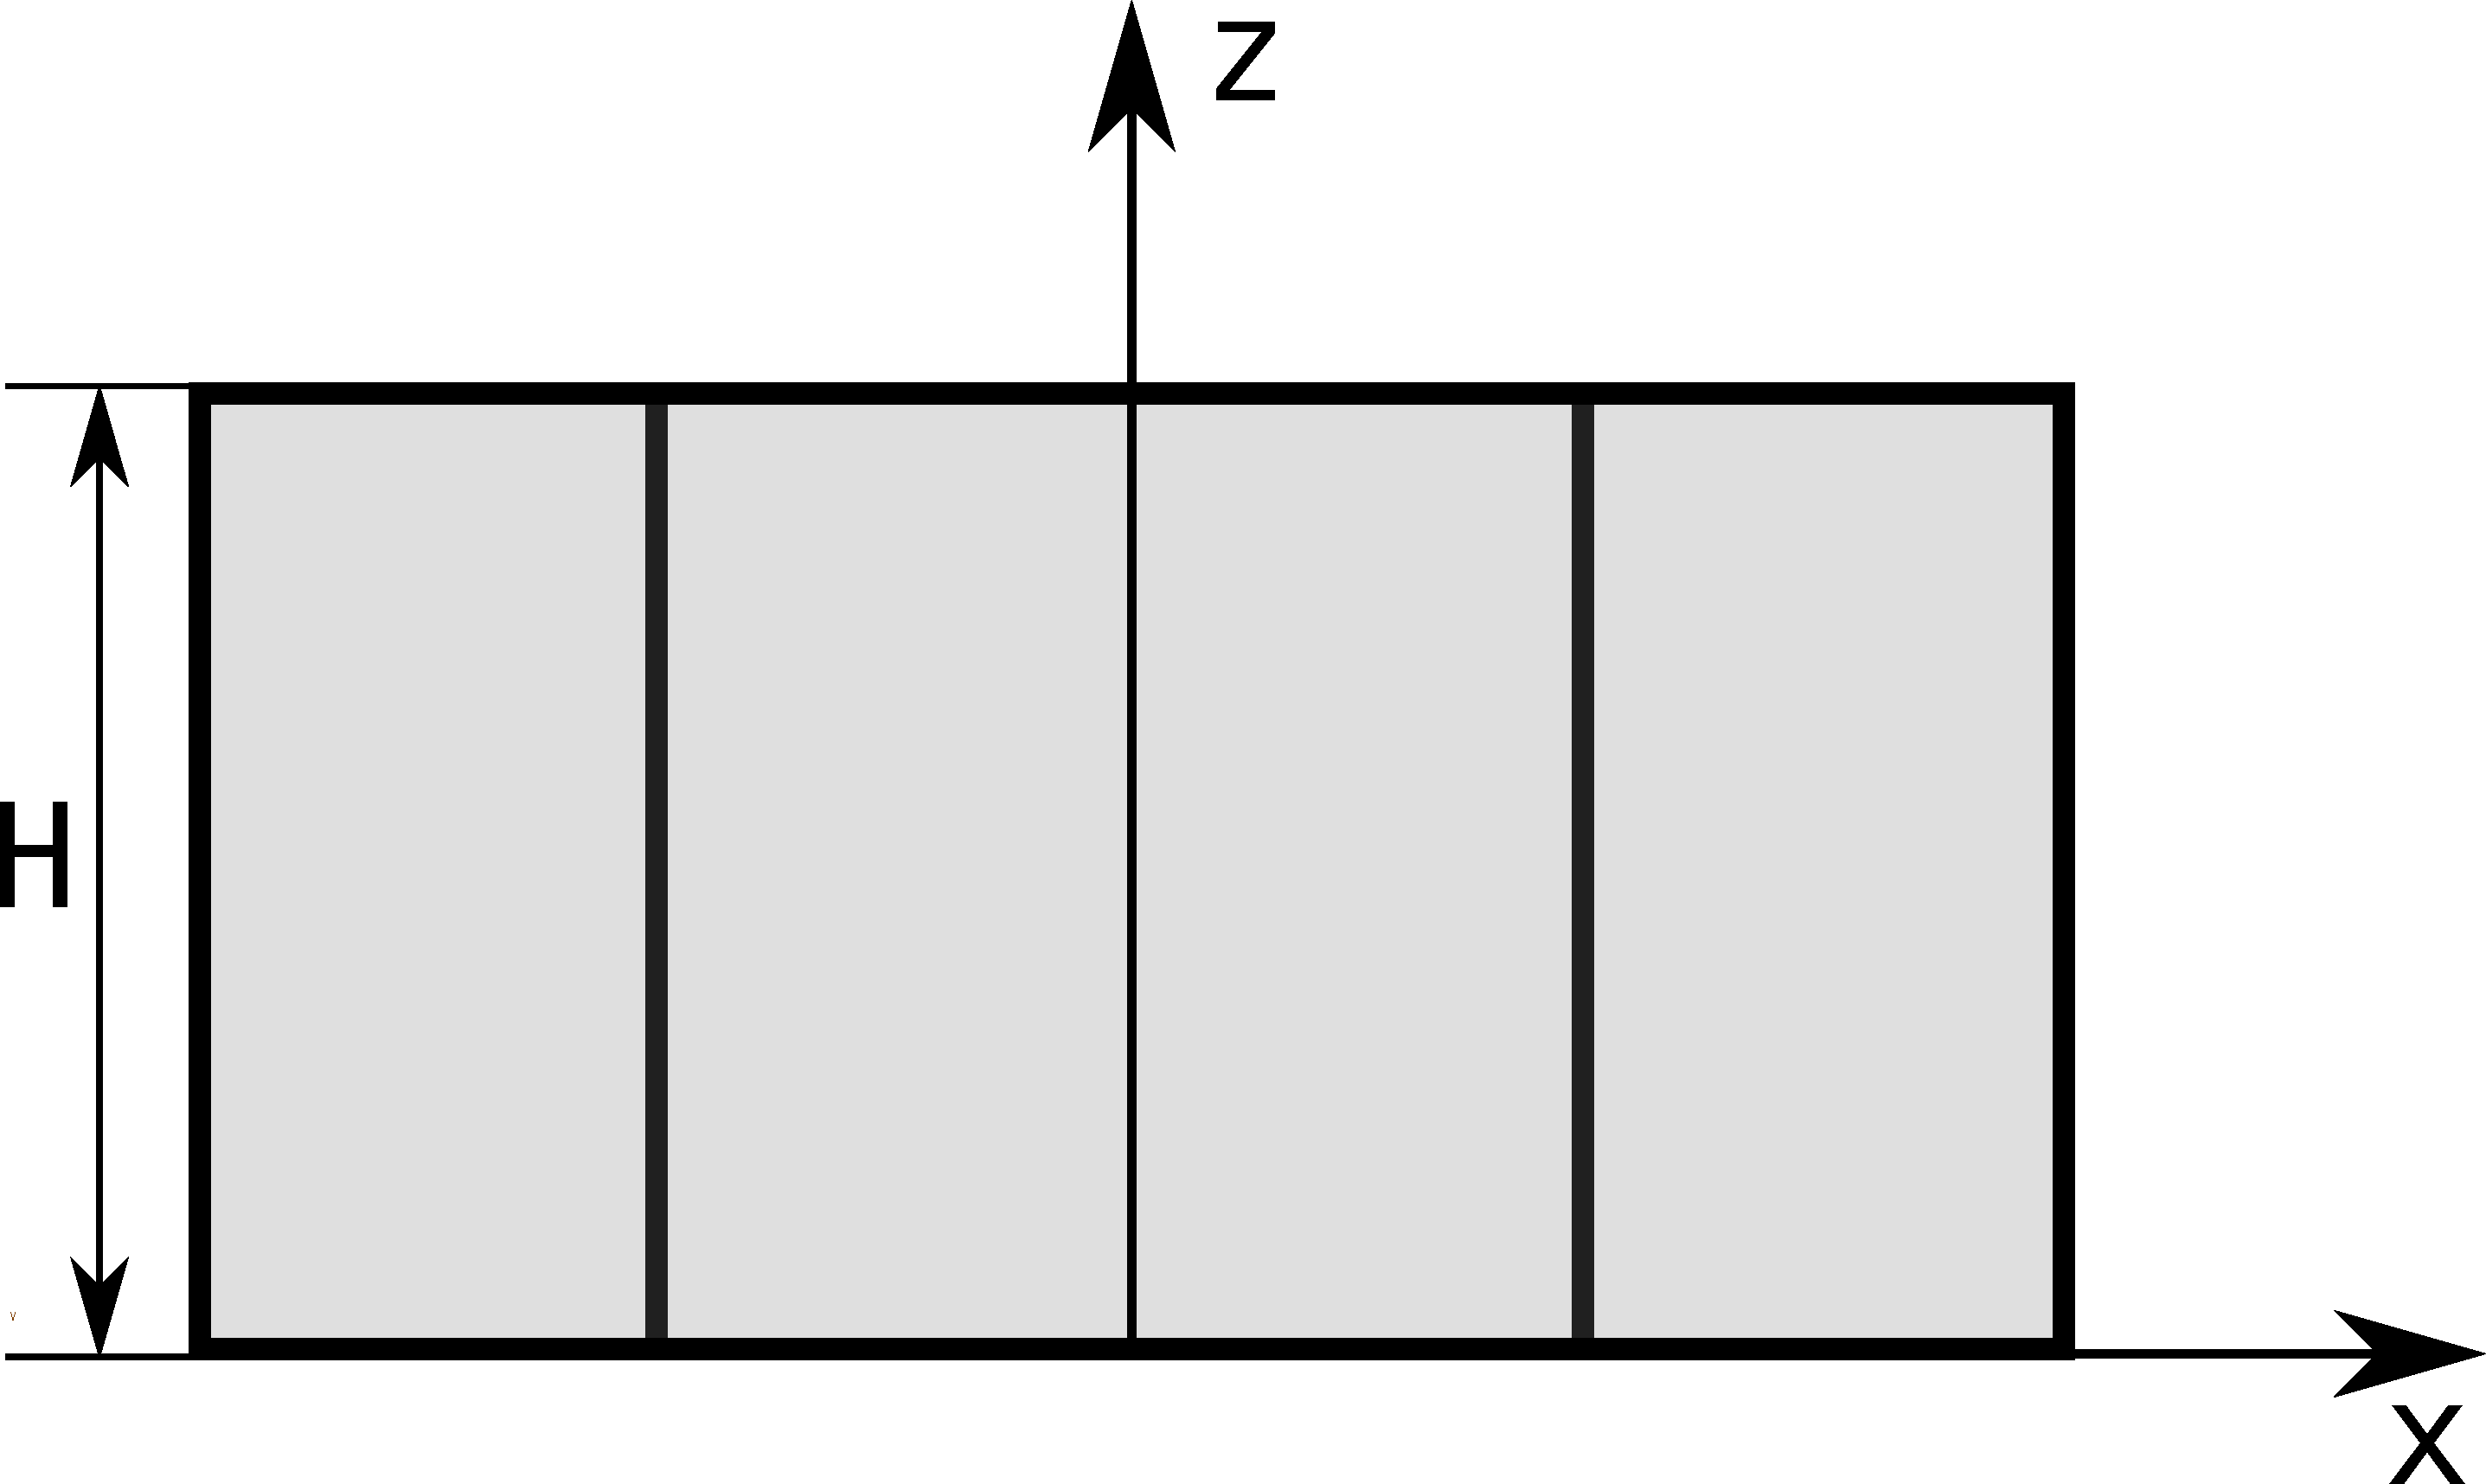
\includegraphics[width=.30\textwidth]{fig/cuts/Prism62dxz.pdf}}}
\hfill
\caption{A prism based on a regular hexagon.}
\end{figure}

\FloatBarrier

\paragraph{Syntax and parameters}\strut\\[-2ex plus .2ex minus .2ex]
\begin{lstlisting}[language=python, style=eclipseboxed,numbers=none,nolol]
  FormFactorPrism6(radius, height)
\end{lstlisting}
with the parameters
\begin{itemize}
\item \texttt{radius} of the hexagonal base, $R$,
\item \texttt{height}, $H$.
\end{itemize}


\paragraph{Form factor etc}\strut\\
\begin{align*}
F &= \frac{4H\sqrt{3}}{3q_y^2 - q_x^2}
\sinc\left(q_z\frac{H}{2}\right) \exp\left(-i q_z\frac{ H}{2}\right)\times\\
&\left\{\frac{3q_y^2R^2}{4} \sinc\left(\frac{q_x
  R}{2}\right)\sinc\left(\frac{\sqrt{3}q_yR }{2}\right)+ \cos(q_x R)-\cos\left(q_y
\frac{\sqrt{3}R}{2}\right) \cos\left(\frac{q_x R}{2}\right)\right\},
\end{align*}
\begin{equation*}
  V = \dfrac{3\sqrt{3}}{2}H R^2,
\end{equation*}
\begin{equation*}
  S =\dfrac{3\sqrt{3}R^2}{2}.
\end{equation*}

\paragraph{Example}\strut\\
Figure~\ref{fig:FFprism6Ex} shows the normalized intensity
$|F|^2/V^2$, computed with $R=5$~nm and \mbox{$H=11$~nm.}

\begin{figure}[H]
\begin{center}
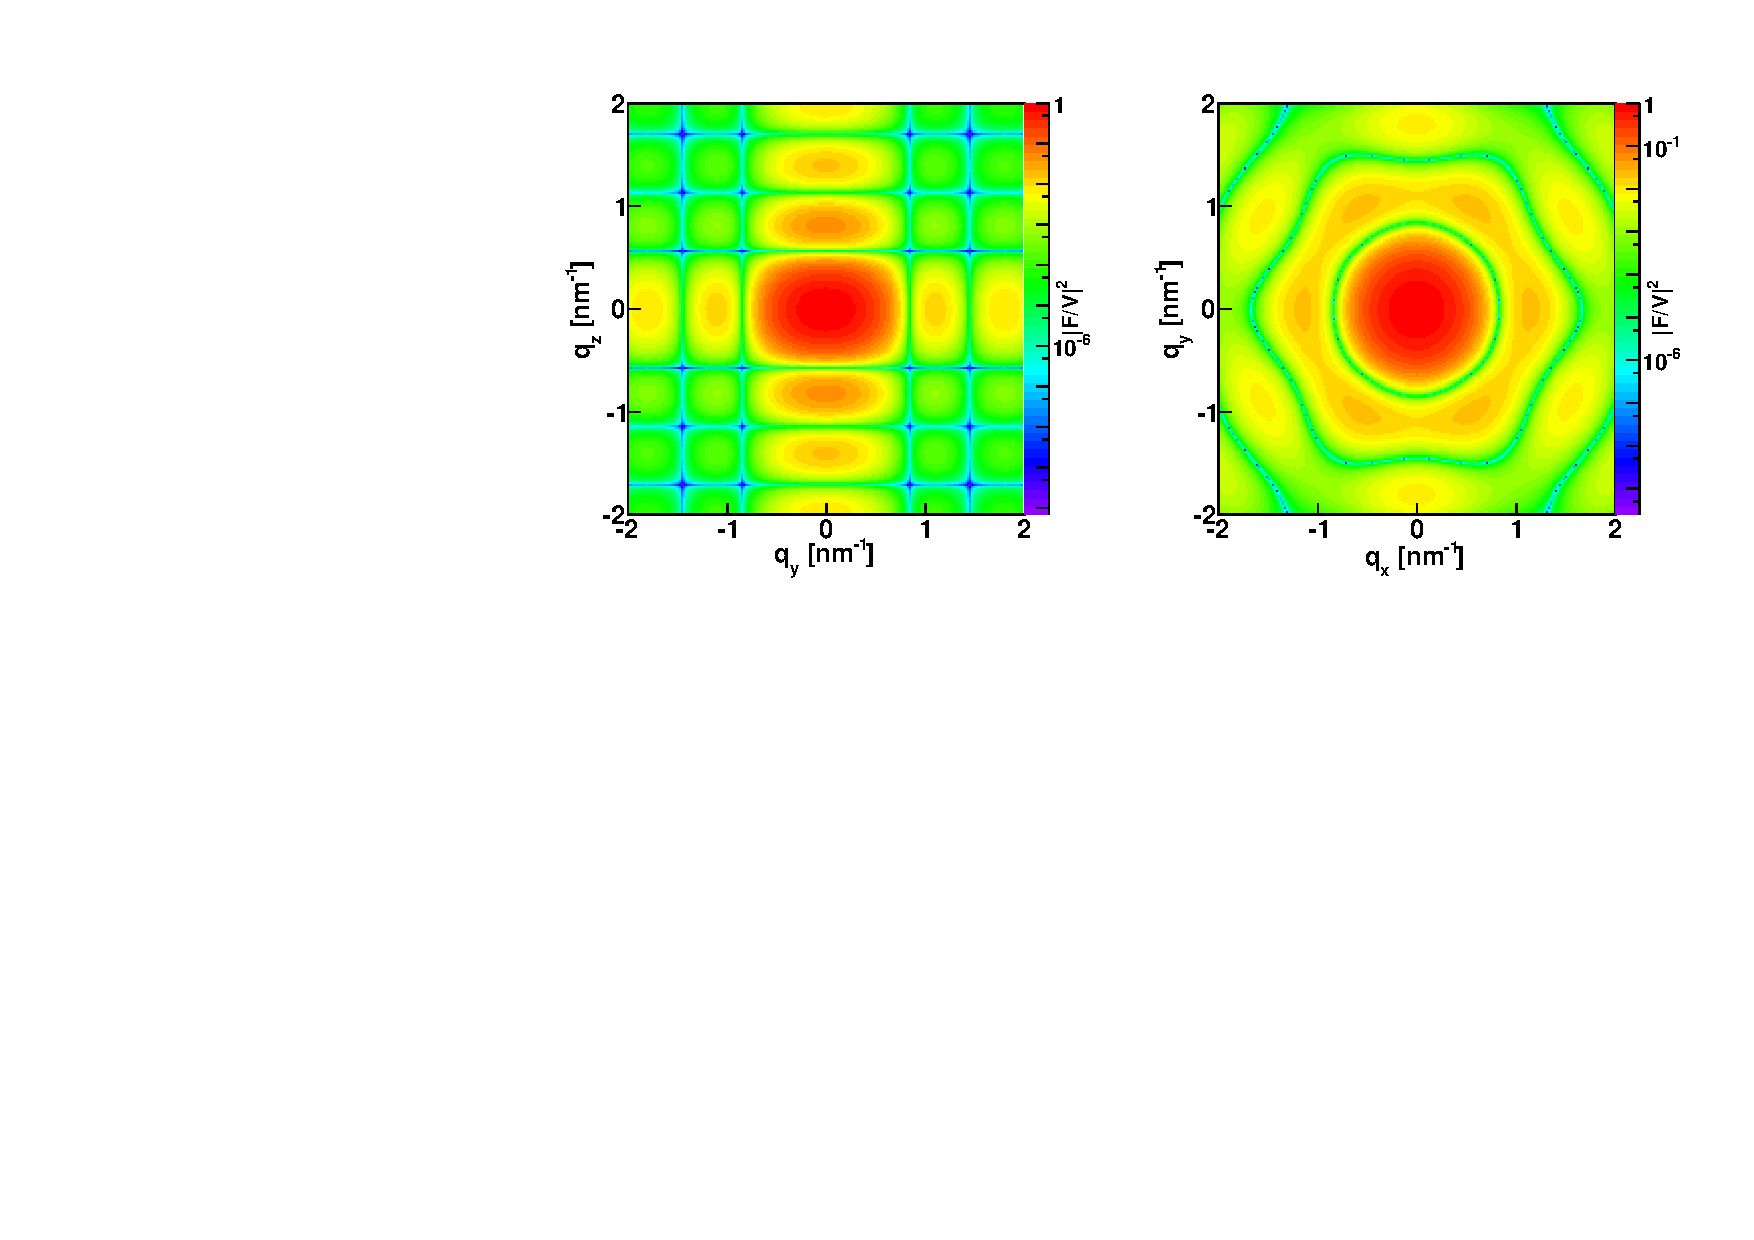
\includegraphics[angle=-90,width=\textwidth]{fig/ff/figffprism6.pdf}
\end{center}
\caption{Normalized intensity for the form factor of a Prism6 plotted against ($q_y$, $q_z$) and ($q_x$, $q_y$) and computed with \Code{FormFactorPrism6(5.*nanometer, 11.*nanometer)}.}
\label{fig:FFprism6Ex}
\end{figure}

\paragraph{References}\strut\\
Corresponds to \E{Prism6} form factor of \IsGISAXS\
\cite[Eq.~2.31]{Laz08} \cite[Eq.~221]{ReLL09},
which has different parametrization
and lacks a factor $H$ in $F(\q)$.

%-------------------------------------------------------------------------------
\clearpage
\subsection{Pyramid (square-based)}\label{sec:Pyramid}
  \index{Pyramid (form factor)!square}
  \index{Truncated pyramid (form factor)!square}
  \index{FormFactorPyramid@\Code{FormFactorPyramid}}
%-------------------------------------------------------------------------------

\paragraph{Real-space geometry}\strut\\

\begin{figure}[H]
\hfill
\subfigure[Perspective]{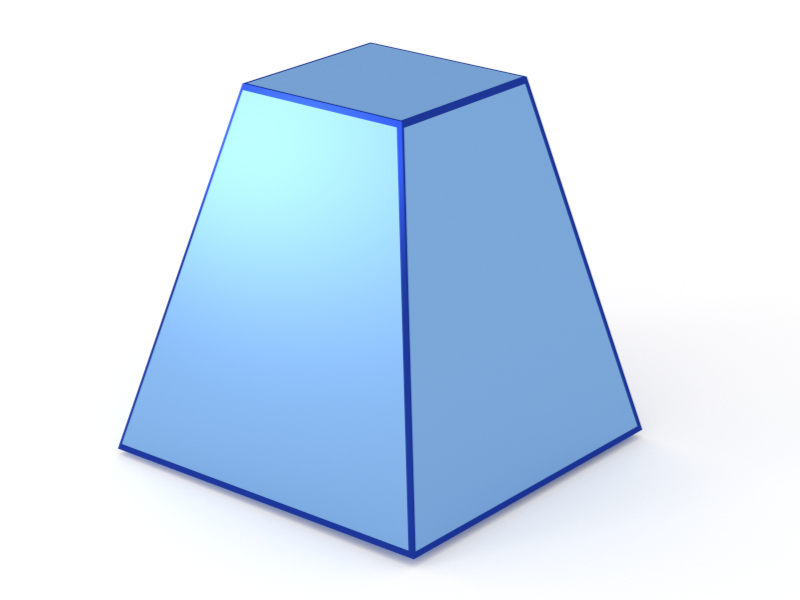
\includegraphics[width=.24\textwidth]{fig/blue/Pyramid3d.png}}
\hfill
\subfigure[Top view]{\includegraphics[width=.30\textwidth]{fig/cuts/Pyramid2dxy.pdf}}
\hfill
\subfigure[Side view]{\raisebox{2mm}{\includegraphics[width=.30\textwidth]{fig/cuts/Pyramid2dxz.pdf}}}
\hfill
\caption{A truncated pyramid with a square base.}
\end{figure}

\FloatBarrier

\paragraph{Syntax and parameters}\strut\\[-2ex plus .2ex minus .2ex]
\begin{lstlisting}[language=python, style=eclipseboxed,numbers=none,nolol]
  FormFactorPyramid(length, height, alpha)
\end{lstlisting}
with the parameters
\begin{itemize}
\item \texttt{length} of one edge of the square base, $L$,  
\item \texttt{height}, $H$,
\item \texttt{alpha}, angle between the base and a side face, $\alpha$,
\end{itemize}
They must fulfill
\begin{displaymath}
  H \le \frac{\tan\alpha}{2}L.
\end{displaymath}


\paragraph{Form factor etc}\strut\\
Notation:
\begin{displaymath}
  \ell\coloneqq L/2,\quad
  h\coloneqq H/2,\quad
  f_\pm(z)\coloneqq \exp(\pm i z)\sinc(z).
\end{displaymath}
Results:
\begin{equation*}
\begin{array}{@{}l@{}l@{}}
\DS F=
\frac{H}{q_xq_y} \Big\{
   &+\DS  f_+\left(\left(\frac{q_x-q_y}{\tan\alpha} +q_z\right)h\right)
        \exp(-i(q_x-q_y)\ell)
\\[3.6ex]
   &\DS+ f_-\left(\left(\frac{q_x-q_y}{\tan\alpha} -q_z\right)h\right)
        \exp(+i(q_x-q_y)\ell)
\\[3.6ex]
   &\DS- f_+\left(\left(\frac{q_x+q_y}{\tan\alpha} +q_z\right)h\right)
        \exp(-i(q_x+q_y)\ell)
\\[3.6ex]
   &\DS- f_-\left(\left(\frac{q_x+q_y}{\tan\alpha} -q_z\right)h\right)
        \exp(+i(q_x+q_y)\ell)
\Big\},
\end{array}
\end{equation*}
\begin{equation*}
  V= H \Big[L^2 - \frac{2LH}{\tan\alpha} + \dfrac{4}{3} \dfrac{H^2}{\tan^2\alpha}\Big].
\end{equation*}
\begin{equation*}
  S=L^2.
\end{equation*}
\begin{equation*}
  V = \dfrac{1}{6}  L^3 \tan\alpha\left[ 1
             - \left(1 - \dfrac{2H}{L\tan\alpha}\right)^3 \right],,
\end{equation*}
\begin{equation*}
  S = L^2.
\end{equation*}

\paragraph{Examples}
Figure~\ref{fig:FFPyramidEx} shows the normalized intensity
$|F|^2/V^2$, computed with $L=18$~nm, $H=13$~nm and
$\alpha=60^{\circ}$.

\begin{figure}[H]
\begin{center}
%\includegraphics[angle=-90,width=\textwidth]{fig/ff/figffpyramid.pdf}
\includegraphics[width=\textwidth]{fig/ff2/ff_pyramid.pdf}
\end{center}
\caption{Normalized intensity for the form factor of a
  pyramid plotted against ($q_y$, $q_z$) and  
  ($q_x$, $q_y$) and computed with  \Code{FormFactorPyramid(18.*nanometer, 13.*nanometer, 60.*degree)}.}
\label{fig:FFPyramidEx}
\end{figure}

\paragraph{References}\strut\\
Corresponds to \E{Pyramid} form factor of \IsGISAXS\
\cite[Eq.~2.31]{Laz08} \cite[Eq.~221]{ReLL09},
with different parametrization $L=2R_{\rm{\Code{IsGISXAXS}}}$,
with correction of a sign error,
and with a more compact form of $F(\q)$.

%-------------------------------------------------------------------------------
\clearpage
\subsection{Ripple1 (sinusoidal)} \label{sec:Ripple1}  
  \index{Ripple (form factor)!sinusoidal (Ripple1)}
  \index{Sinusoidal ripple (form factor)}
  \index{FormFactorRipple1@\Code{FormFactorRipple1}}
%-------------------------------------------------------------------------------

\paragraph{Real-space geometry}\strut\\

\begin{figure}[H]
\hfill
\subfigure[Perspective]{\includegraphics[width=.24\textwidth]{fig/blue/Ripple13d.png}}
\hfill
\subfigure[Top view]{\includegraphics[width=.30\textwidth]{fig/cuts/Ripple12dxy.pdf}}
\hfill
\subfigure[Side view]{\includegraphics[width=.30\textwidth]{fig/cuts/Ripple12dyz.pdf}}
\hfill
\caption{An infinite ripple with a sinusoidal profile.}
\end{figure}

\paragraph{Syntax and parameters}\strut\\[-2ex plus .2ex minus .2ex]
\begin{lstlisting}[language=python, style=eclipseboxed,numbers=none,nolol]
  FormFactorRipple1(length, width, height)
\end{lstlisting}
with the parameters
\begin{itemize}
\item \texttt{length}, $L$, 
\item \texttt{width}, $W$, 
\item \texttt{height}, $H$. 
\end{itemize}


\paragraph{Form factor etc}\strut\\
\begin{align*}
F &=L \cdot \frac{W}{\pi}\cdot \sinc\left(\frac{q_xL}{2}\right)\times \\
&\int_0^H\!\d z\, \arccos\left(\frac{2z}{H}-1\right)\sinc\left[\frac{q_yW}{2\pi}\arccos\left(\frac{2z}{H} - 1\right)\right]\exp\left(iq_zz\right),
\end{align*}
\begin{equation*}
  V = \dfrac{L W H}{2},
\end{equation*}
\begin{equation*}
  S = L W.
\end{equation*}

\paragraph{Example}\strut\\
Figure~\ref{fig:FFripple1Ex} shows the normalized intensity
$|F|^2/V^2$, computed with $L=27$~nm, $W=20$~nm and $H=14$~nm.

\begin{figure}[H]
\begin{center}
\includegraphics[angle=-90,width=\textwidth]{fig/ff/figffripple1.pdf}
\end{center}
\caption{Normalized intensity for the form factor of a ripple1
  $|F|^2/V^2$, plotted against ($q_y$, $q_z$) and  ($q_x$, $q_y$)
  computed with \Code{FormFactorRipple1(27.*nanometer, 20.*nanometer, 14.*nanometer)}.}
\label{fig:FFripple1Ex}
\end{figure}


%-------------------------------------------------------------------------------
\clearpage
\subsection{Ripple2 (saw-tooth)} \label{sec:Ripple2}  
  \index{Ripple (form factor)!saw-tooth (Ripple2)}
  \index{Saw-tooth ripple (form factor)}
  \index{FormFactorRipple2@\Code{FormFactorRipple2}}
%-------------------------------------------------------------------------------

\paragraph{Real-space geometry}\strut\\

\begin{figure}[H]
\hfill
\subfigure[Perspective]{\includegraphics[width=.24\textwidth]{fig/blue/Ripple23d.png}}
\hfill
\subfigure[Top view]{\includegraphics[width=.30\textwidth]{fig/cuts/Ripple22dxy.pdf}}
\hfill
\subfigure[Side view]{\includegraphics[width=.30\textwidth]{fig/cuts/Ripple22dyz.pdf}}
\hfill
\caption{An infinite ripple with an asymmetric saw-tooth profile.}
\end{figure}

\FloatBarrier

\paragraph{Syntax and parameters}\strut\\[-2ex plus .2ex minus .2ex]
\begin{lstlisting}[language=python, style=eclipseboxed,numbers=none,nolol]
  FormFactorRipple2(length, width, height, asymmetry)
\end{lstlisting}
with the parameters
\begin{itemize}
\item \texttt{length}, $L$, 
\item \texttt{width}, $W$, 
\item \texttt{height}, $H$. 
\item \texttt{asymmetry}, $d$. 
\end{itemize}
They must fulfill
\begin{displaymath}
  |d| \le W/2.
\end{displaymath}


\paragraph{Form factor etc}\strut\\
\begin{align*}
F &=L W
\sinc\left(\frac{q_xL}{2}\right)\times \\ &
\int_0^H \!\d z\,
\left(1-\frac{z}{H}\right)
 \sinc\left[\frac{q_y
    W}{2}\left(1-\frac{z}{H}\right)\right] 
\exp\left\{ i\left[q_zz -
    q_yd\left(1-\frac{z}{H}\right)\right]\right\}
\end{align*}
\begin{equation*}
  V = \dfrac{L W H}{2},
\end{equation*}
\begin{equation*}
  S = L W.
\end{equation*}

\paragraph{Examples}
Figure~\ref{fig:FFripple2Ex} shows the normalized intensity
$|F|^2/V^2$, computed with $L=36$~nm, $W=25$~nm, $H=14$~nm, and $d=3$~nm.

\begin{figure}[H]
\begin{center}
\includegraphics[angle=-90,width=\textwidth]{fig/ff/figffripple2.pdf}
\end{center}
\caption{Normalized intensity for the form factor of a ripple2 plotted against ($q_y$, $q_z$) and  ($q_x$, $q_y$)
  computed with \Code{FormFactorRipple2(36.*nanometer, 25.*nanometer, 14.*nanometer, 3.*nanometer)}.}
\label{fig:FFripple2Ex}
\end{figure}

%-------------------------------------------------------------------------------
\clearpage
\subsection{Tetrahedron} \label{sec:Tetrahedron}
  \index{Tetrahedron (form factor)}
  \index{Truncated tetrahedron (form factor)}
  \index{FormFactorTetrahedron@\Code{FormFactorTetrahedron}}
%-------------------------------------------------------------------------------
 
\paragraph{Real-space geometry}\strut\\

\begin{figure}[H]
\hfill
\subfigure[Perspective]{\includegraphics[width=.24\textwidth]{fig/blue/Tetrahedron3d.png}}
\hfill
\subfigure[Top view]{\includegraphics[width=.30\textwidth]{fig/cuts/Tetrahedron2dxy.pdf}}
\hfill
\subfigure[Side view]{\raisebox{5mm}{\includegraphics[width=.30\textwidth]{fig/cuts/Tetrahedron2dxz.pdf}}}
\hfill
\caption{A truncated tetrahedron.}
\end{figure}

\FloatBarrier

\paragraph{Syntax and parameters}\strut\\[-2ex plus .2ex minus .2ex]
\begin{lstlisting}[language=python, style=eclipseboxed,numbers=none,nolol]
  FormFactorTetrahedron(length, height, alpha)
\end{lstlisting}
with the parameters
\begin{itemize}
\item \texttt{length} of one edge of the equilateral triangular base, $L$,
\item \texttt{height}, $H$,
\item \texttt{alpha}, angle between the base and a side face, $\alpha$.
\end{itemize}
They must fulfill
\begin{displaymath}
  H\le \frac{\tan{\alpha}}{2\sqrt{3}} L.
\end{displaymath}
Note that the orthographic projection does not show~$\alpha$,
but the angle~$\beta$ between the base and a side edge.
They are related through $\tan \alpha = 2 \tan \beta$. 


\paragraph{Form factor etc}\strut\\
Notation:
\begin{equation*}
q_1  \coloneqq \frac{1}{2}\left[\frac{q_x\sqrt{3} -q_y}{\tan \alpha}-q_z \right],
\quad q_2 \coloneqq \frac{1}{2}\left[\frac{q_x\sqrt{3} +q_y}{\tan \alpha}+q_z
\right], \quad 
q_3 \coloneqq \frac{q_y}{\tan \alpha} -\frac{q_z}{2}, \quad 
D \coloneqq \frac{L \tan \alpha}{\sqrt{3}} -H.
\end{equation*}
Results:
\begin{align*}
&F=\frac{\sqrt{3}H}{q_x (q_x^2-3q_y^2)}
\exp\left(i\frac{q_z L\tan (\alpha)}{2\sqrt{3}}\right) \times \\
&\Big\{2q_x \exp(iq_3 D)\sinc(q_3 H) - (q_x +\sqrt{3}q_y)
\exp(iq_1 D)\sinc(q_1 H)\\
&-(q_x-\sqrt{3}q_y)\exp(-iq_2 D)\sinc(q_2 H) \Big\}, 
\end{align*}
\begin{equation*}
  V= \dfrac{\tan(\alpha) L^3}{24} \left[1- \left(1 -
  \dfrac{2\sqrt{3} H}{L \tan(\alpha)} \right)^3\right],
\end{equation*}
\begin{equation*}
  S =\dfrac{\sqrt{3}}{4}L^2.
\end{equation*}

\paragraph{Example}\strut\\
Figure~\ref{fig:FFtetrahEx} shows the normalized intensity
$|F|^2/V^2$, computed with $L=15$~nm, $H=6$~nm and $\alpha =60
^{\circ}$.

\begin{figure}[H]
\begin{center}
\includegraphics[angle=-90,width=\textwidth]{fig/ff/figfftetrahedron.pdf}
\end{center}
\caption{Normalized intensity for the form factor of a Tetrahedron
  plotted against ($q_y$, $q_z$) and  ($q_x$, $q_y$) and
  computed with \Code{FormFactorTetrahedron(15.*nanometer, 6.*nanometer, 60.*degree)}.}
\label{fig:FFtetrahEx}
\end{figure}

\paragraph{References}\strut\\
Agrees with the \E{Tetrahedron} form factor of \IsGISAXS\
\cite[Eq.~2.30]{Laz08} \cite[Eq.~220]{ReLL09}.


%-------------------------------------------------------------------------------
\clearpage
\subsection{TruncatedCube} \label{sec:TruncatedCube}  
\index{Cube (form factor)!truncated}
  \index{Truncated cube (form factor)}
  \index{FormFactorTruncatedCube@\Code{FormFactorTruncatedCube}}
%-------------------------------------------------------------------------------

\paragraph{Real-space geometry}\strut\\

\begin{figure}[H]
\hfill
\subfigure[Perspective]{\includegraphics[width=.24\textwidth]{fig/blue/TruncatedCube3d.png}}
\hfill
\subfigure[Top view]{\includegraphics[width=.30\textwidth]{fig/cuts/Truncatedcube2dxy.pdf}}
\hfill
\subfigure[Side view]{\includegraphics[width=.30\textwidth]{fig/cuts/Truncatedcube2dxz.pdf}}
\hfill
\caption{A cube whose eight vertices have been removed.
The truncated part of each vertex is a trirectangular tetrahedron.}
\end{figure}

\FloatBarrier

\paragraph{Syntax and parameters}\strut\\[-2ex plus .2ex minus .2ex]
\begin{lstlisting}[language=python, style=eclipseboxed,numbers=none,nolol]
  FormFactorTruncatedCube(length, removed_length)
\end{lstlisting}
with the parameters
\begin{itemize}
\item \texttt{length} of the full cube, $L$,
\item \texttt{removed\_length}, side length of the trirectangular tetrahedron removed from the cube's vertices, $t$.
\end{itemize}
They must fulfill
\begin{displaymath}
  t \le L/2.
\end{displaymath}


\paragraph{Form factor etc}\strut\\
Notation:\\
Besides the form factor $F_\text{Box}(\q)$
of the full cube of side length $L$ (Sect.~\ref{sec:Box}),
we need the form factor of a trirectangular tetrahedrons
as cut from the cube:
\begin{align*}
F_{\text{vertex}_1}(q_x, q_y, q_z, L, t) &=\frac{t}{q_z}\exp\left( i\frac{q_x(L-t)+ q_y L}{2} \right) \\
\times \Big\{ \frac{1}{q_y} \sinc\left( \frac{q_x t}{2}\right)
&- \frac{q_z}{q_y(q_y + q_z)} \exp\left(i\frac{q_yt}{2}\right) \sinc\left( \frac{(q_x-q_y)t}{2}\right)\\
&- \frac{1}{q_y + q_z} \exp\left( i\frac{q_z t}{2} \right) \sinc \left( \frac{(q_x+q_z) t}{2} \right)  \Big\}    
\end{align*}
Thanks to symmetry (see the following figure,
which shows the vertices $V_i$ for $i=1,\ldots,8$),
the form factors of other seven tetrahedrons cut from the cube
can be computed as follows
(note that the origin is taken as usual
at the centre of the bottom face of the cube):
\begin{figure}[H]
\begin{center}
\includegraphics[width=.5\textwidth]{fig/drawing/SketchTruncatedcube.png}
\end{center}
\end{figure}
\begin{align*}
F_{\text{vertex}_2}(q_x, q_y, q_z, L, t) &= F_{\text{vertex}_1}(q_y, -q_x, q_z, L, t) \\
F_{\text{vertex}_3}(q_x, q_y, q_z, L, t) &= F_{\text{vertex}_1}(-q_x, -q_y, q_z, L, t) \\
F_{\text{vertex}_4}(q_x, q_y, q_z, L, t) &= F_{\text{vertex}_1}(-q_y, q_x, q_z, L, t) \\
F_{\text{vertex}_5}(q_x, q_y, q_z, L, t) &= \exp(iq_zL)F_{\text{vertex}_1}(q_x, q_y, -q_z, L, t) \\
F_{\text{vertex}_6}(q_x, q_y, q_z, L, t) &= \exp(iq_zL)F_{\text{vertex}_1}(q_y, -q_x,- q_z, L, t) \\
F_{\text{vertex}_7}(q_x, q_y, q_z, L, t) &= \exp(iq_zL)F_{\text{vertex}_1}(-q_x, -q_y, -q_z, L, t) \\
F_{\text{vertex}_8}(q_x, q_y, q_z, L, t) &= \exp(iq_zL)F_{\text{vertex}_1}(-q_y, q_x, -q_z, L, t)
\end{align*}
Result:
\begin{equation*}
F =F_{\text{Box}}(q_x,q_y,q_z, L, L, L) - \sum_{i=1}^8 F_{\text{vertex}_i}(q_x, q_y, q_z, L, t)
\end{equation*}
\begin{equation*}
  V = L^3 - \dfrac{4}{3}t^3,
\end{equation*}
\begin{equation*}
  S = L^2.
\end{equation*}

\paragraph{Examples}
Figure~\ref{fig:FFtrunccubeEx} shows the normalized intensity
$|F|^2/V^2$, computed with $L=15$~nm  and $t=6$~nm.

\begin{figure}[H]
\begin{center}
\includegraphics[angle=-90,width=\textwidth]{fig/ff/figfftruncatedcube.pdf}
\end{center}
\caption{Normalized intensity for the form factor of a truncated cube plotted against ($q_y$, $q_z$) and  ($q_x$, $q_y$)
  computed with \Code{FormFactorTruncatedCube(15.*nanometer, 6.*nanometer)}.}
\label{fig:FFtrunccubeEx}
\end{figure}

\paragraph{References}\strut\\
\cite{HeSS74}

%-------------------------------------------------------------------------------
\clearpage
\subsection{TruncatedSphere}\label{sec:TruncatedSphere}
  \index{Sphere (form factor)!truncated}
  \index{Truncated sphere (form factor)}
  \index{FormFactorTruncatedSphere@\Code{FormFactorTruncatedSphere}}
%-------------------------------------------------------------------------------
  
\paragraph{Real-space geometry}\strut\\

\begin{figure}[H]
\hfill
\subfigure[Perspective]{\includegraphics[width=.24\textwidth]{fig/blue/Sphere3d.png}}
\hfill
\subfigure[Top view]{\includegraphics[width=.30\textwidth]{fig/cuts/Sphere2dxy.pdf}}
\hfill
\subfigure[Side view]{\raisebox{-2mm}{\includegraphics[width=.30\textwidth]{fig/cuts/Sphere2dxz.pdf}}}
\hfill
\caption{A truncated sphere.}
\end{figure}
\FloatBarrier

\paragraph{Syntax and parameters}\strut\\[-2ex plus .2ex minus .2ex]
\begin{lstlisting}[language=python, style=eclipseboxed,numbers=none,nolol]
  FormFactorTruncatedSphere(radius, height)
\end{lstlisting}
with the parameters
\begin{itemize}
\item \texttt{radius}, $R$,
\item \texttt{height}, $H$.
\end{itemize}
They must fulfill
\begin{displaymath}
   0 < H\leq 2R.
\end{displaymath}


\paragraph{Form factor etc}\strut\\
Notation:
\begin{equation*}
  q_{\parallel} \coloneqq \sqrt{q_x^2+q_y^2},\quad
  R_z \coloneqq \sqrt{R^2-z^2}.
\end{equation*}
Results:
\begin{equation*}  
F= 2\pi \exp[i q_z (H-R)]\int_{R-H}^{R}\!\d z\, R_z^2
       \frac{J_1(q_{\parallel} R_z) }{q_{\parallel} R_z} \exp(i q_z z) dz,
\end{equation*}
\begin{equation*}
  V=\pi R^3 \left[\dfrac{2}{3} + \dfrac{H-R}{R} - \dfrac{1}{3}\left(\dfrac{H-R}{R}\right)^3\right],
\end{equation*}
\begin{equation*}
  S = \left\{\begin{array}{ll} \pi R^2, & H \geq R \\
         \pi\left(2RH-H^2\right), & H < R \end{array}\right..
\end{equation*}

\paragraph{Example}\strut\\
Figure~\ref{fig:SphereEx} shows the normalized intensity $|F|^2/V^2$, computed with $R=5$~nm and $H=7$~nm:
\begin{figure}[H]
\begin{center}
\includegraphics[angle=-90,width=\textwidth]{fig/ff/figffsphere.pdf}
\end{center}
\caption{Normalized intensity for the form factor of a Truncated Sphere plotted against ($q_y$, $q_z$) and ($q_x$, $q_y$) and
  computed with \Code{FormFactorTruncatedSphere(5.*nanometer, 7.*nanometer)}.}
\label{fig:SphereEx}
\end{figure}

\paragraph{References}\strut\\
Agrees with the \IsGISAXS\ form factor
\E{Sphere} \cite[Eq.~2.33]{Laz08} or
\E{Truncated sphere} \cite[Eq.~228]{ReLL09}.

%-------------------------------------------------------------------------------
\clearpage
\subsection{TruncatedSpheroid} \label{sec:TruncatedSpheroid}
  \index{Spheroid (form factor)!truncated}
  \index{Truncated spheroid (form factor)}
  \index{FormFactorTruncatedSpheroid@\Code{FormFactorTruncatedSpheroid}}
%-------------------------------------------------------------------------------

\paragraph{Real-space geometry}\strut\\

\begin{figure}[H]
\hfill
\subfigure[Perspective]{\includegraphics[width=.24\textwidth]{fig/blue/Spheroid3d.png}}
\hfill
\subfigure[Top view]{\raisebox{5mm}{\includegraphics[width=.30\textwidth]{fig/cuts/Spheroid2dxy.pdf}}}
\hfill
\subfigure[Side view]{\includegraphics[width=.30\textwidth]{fig/cuts/Spheroid2dxz.pdf}}
\hfill
\caption{A vertically oriented, horizontally truncated spheroid.}
\end{figure}

\paragraph{Syntax and parameters}\strut\\[-2ex plus .2ex minus .2ex]
\begin{lstlisting}[language=python, style=eclipseboxed,numbers=none,nolol]
  FormFactorTruncatedSpheroid(radius, height, height_flattening)
\end{lstlisting}
with the parameters
\begin{itemize}
\item \texttt{radius}, $R$,
\item \texttt{height}, $H$.
\item \texttt{height\_flattening}, $f_p$.
\end{itemize}
They must fulfill
\begin{displaymath}
  0< \dfrac{H}{R}\le 2f_p.
\end{displaymath}


\paragraph{Form factor etc}\strut\\
Notation:
\begin{equation*} 
  q_{\parallel} \coloneqq \sqrt{q_x^2+q_y^2}, \quad
  R_z \coloneqq \sqrt{R^2-z^2/f_p^2}.
\end{equation*} 
Results:
\begin{equation*} 
F =   2\pi \exp[iq_z(H-f_pR)] \int_{f_p R-H}^{f_p R} \!\d z\,
     R_z^2\frac{J_1(q_{\parallel}R_z)}{q_{\parallel}R_z} \exp(i q_z z) 
\end{equation*}
\begin{equation*}
  V = \dfrac{\pi R H^2}{f_p}  \Big(1-\dfrac{H}{3f_p R}\Big),
\end{equation*}
\begin{equation*}
  S = \left\{\begin{array}{ll} \pi R^2, & H \geq f_pR \\
         \pi\left(\dfrac{2RH}{f_p}-\dfrac{H^2}{f_p^2}\right), & H < R \end{array}\right..
\end{equation*}

\paragraph{Example}\strut\\
Figure~\ref{fig:FFspheroidEx} shows the normalized intensity
$|F|^2/V^2$, computed with $R=7.5$~nm, $H=9$~nm and $f_p=1.2$.

\begin{figure}[H]
\begin{center}
\includegraphics[angle=-90,width=\textwidth]{fig/ff/figffspheroid.pdf}
\end{center}
\caption{Normalized intensity for the form factor of a Truncated Spheroid plotted against ($q_z$, $q_y$) and ($q_x$, $q_y$) and
  computed with \Code{FormFactorTruncatedSpheroid(7.5*nanometer, 9.*nanometer, 1.2)}.}
\label{fig:FFspheroidEx}
\end{figure}

\paragraph{References}\strut\\
Agrees with the \IsGISAXS\ form factor
\E{Sphere} \cite[Eq.~2.33]{Laz08} or
\E{TruncatedSpheroid} \cite[Eq.~228]{ReLL09}.
% Note an erroneous factor~2 in the expression of the volume
% in the \Code{IsGISAXS} manual.


\index{Shape transform|)}

%===============================================================================
\clearpage
\section{Core-shell particles} \label{sec:CoreShell}
%===============================================================================
\index{Core-shell particles}

To generate a core-shell particle, the combination is performed using the following command:\\
\Code{ParticleCoreShell(shell\_particle, core\_particle, relative\_core\_position)},\\
where \Code{shell\_particle} and \Code{core\_particle} are the outer and inner parts of the core-shell particle, respectively. They refer to one of the form factors defined previously and to an associated material. For example, for the outer part,\\ \Code{shell\_particle=Particle(material\_shell, outer\_form\_factor)},\\ where \Code{material\_shell} is the material of the shell and \Code{outer\_form\_factor} is the shape of the outer part (cf. listing~\ref{lst:cshellsample}). \\ \Code{relative\_core\_position} defines the position of the inner shape with respect to the outer one; it is defined with respect to the center of the base of the particular form factor. An example in fig.~\ref{fig:coreshell} shows a core shell particle made of a box for the outer part and of a shifted pyramidal shape for the inner one.\\

Figure~\ref{fig:FFCoreShellBA} displays the output intensity scattered in the Born Approximation using the code listed in~\ref{lst:cshellsample} to generate the core-shell particle. 

\begin{figure}[ht]
\hfill
\subfigure[Side view]{\includegraphics[width=.30\textwidth]{fig/cuts/CoreShellParallPyrxz.pdf}}
\hfill
\subfigure[Top view]{\includegraphics[width=.30\textwidth]{fig/cuts/CoreShellParallPyrxy.pdf}}
\hfill
\caption{Example of a core-shell particle composed of a box with a pyramidal  inset. The relative core shell position is marked by the positions of the centers of the bases. }
\label{fig:coreshell}
\end{figure}

\clearpage

\begin{lstlisting}[language=python,
  style=eclipseboxed,numbers=none,nolol,caption={\Code{Python} script
    to create a core-shell particle made of a box with a pyramidal shifted inset.},label={lst:cshellsample}]
    outer_ff = FormFactorBox(16.0*nanometer, 16.0*nanometer, 8.0*nanometer) 
    inner_ff = FormFactorPyramid(12.0*nanometer, 7.0*nanometer, 60.0*degree)
    shell_particle = Particle(m_shell, outer_ff)
    core_particle = Particle(m_core, inner_ff)
    core_position = kvector_t(1.5, 0.0, 0.0)

    particle = ParticleCoreShell(shell_particle, core_particle, core_position)
\end{lstlisting}

\begin{figure}[ht]
\begin{center}
\includegraphics[angle=-90,width=0.6\textwidth]{fig/gisasmap/CoreShellParallPyr.pdf}
\end{center}
\caption{Intensity map of a core-shell form factor in Born Approximation using  \Code{FormFactorBox(16*nanometer, 16*nanometer, 8*nanometer)} and \Code{FormFactorPyramid(12*nanometer, 7*nanometer, 60*degree)} for the outer and inner shells, respectively. The core particle is shifted by 1.5~nm in the $x$-direction with respect to the center of the outer shell. The sample used to generate the particle is listed in~\ref{lst:cshellsample}.  There is no substrate and no interference between the particles.}
\label{fig:FFCoreShellBA}
\end{figure}

\clearpage
%===============================================================================
\section{Rotation of particles}
%===============================================================================
\index{Rotation of particles}
\index{Orientation of particles}

The particles can be rotated in a different direction by using one of
the following transformations: \Code{CreateRotateX($\theta$),
  CreateRotateY($\theta$), CreateRotateZ($\theta$)}, where capital X, Y, Z mark rotations
around the associated axis and $\theta$ is the
angle of rotation from this axis. For example, the following \Code{Python}\ script shows how to rotate a pyramid by $45^{\circ}$ around
the $z$-axis:\\

\begin{lstlisting}[language=python, style=eclipseboxed,numbers=none,nolol]
    pyramid_ff = FormFactorPyramid(10*nanometer, 5*nanometer, deg2rad(54.73 ) )
    pyramid = Particle(m_particle, pyramid_ff)
    angle_around_z = 45.*degree
    transform = Transform3D.createRotateZ(angle_around_z)
    particle_layout = ParticleLayout()
    particle_layout.addParticle(pyramid, transform) 
\end{lstlisting}

%===============================================================================
\section{Polydispersity}
%===============================================================================

... to come
\index{Form factor|)}
